\documentclass[custom]{linearbook}
\usepackage{float}
\usepackage{xchoices}

\begin{document}
% \tikzexternaldisable

\frontmatter
\pagenumbering{Alph}
% 封面
%--------------------------------------------------------------------------
\bookmark[page=1, level=1]{封面}

\includepdf[noautoscale=true, width=\paperwidth]{images/cover.pdf}

% 扉页
%--------------------------------------------------------------------------
\pagenumbering{roman}
\setcounter{page}{1}
\pagestyle{front}
\clearsidenotenumber
\newgeometry{includemp=true,
             inner=2cm,outer=2cm,
             top=2cm,bottom=1.5cm,
             headsep=0.5cm,headheight=0.5cm,
             footskip=0.7cm,
             marginparsep=0cm,marginparwidth=0cm}
\thispagestyle{empty}
\bookmark[page=2, level=1]{扉页}

\begin{tikzpicture}[remember picture,overlay]
    \node at (current page.north west)
      {
        \begin{tikzpicture}[remember picture,overlay]
          \draw[fill=lbdeepblue,draw opacity=0]
            ++(0,-2cm) rectangle ++(\paperwidth,-4pt);
          \node[color=lbdeepblue,text width=13cm] (text)
            at  (0.5\paperwidth,-0.25\paperheight)
            {\titlefont\fontsize{48}{80}\selectfont  工科数学分析\\[0.45cm] 入门讲义};
          \node[color=lbdeepgreen,below right,text width=13cm] (V) at ($(text.south west)+(0.5em,-1em)$)
          {\fontsize{13}{15}\selectfont \fontspec{Palatino-Roman} Mathematical Analysis of Engineering\\ Introductory Notes};
          \draw[line width=2pt,color=lbgreen]
            ++(2cm,-2cm) |- ($(text.south east)+(0,-2.5cm)$);
        \end{tikzpicture}
      };
\end{tikzpicture}

\vspace*{10cm}

\hspace{0.15\linewidth}\begin{minipage}{0.71\linewidth}
  % \zihao{5}
  \begin{flushright}\fontspec{Palatino-Roman}\selectfont\titlefont
    彭康书院学业辅导与发展中心志愿者部~~编写
\date{\zhtoday}  
\end{flushright}
\end{minipage}

\vfill

\begin{figure}[H]
	\centering
	
\includegraphics[scale=0.1]{xdt-logo.png}
\end{figure}

\restoregeometry

% 版权页
%--------------------------------------------------------------------------
%\input{other/copyright.tex}

% 作者简介
%--------------------------------------------------------------------------
\chapter*{编写人员简介}
\addcontentsline{toc}{chapter}{编写人员简介}

\vspace{-3cm}

(按首拼字母排序)

\vspace{1em}

{\zihao{-2}\color{lbdeepblue}司秉钤}\quad 数试2101班学生,彭康学导团志愿者,在本份讲义中负责第一部分第4、5、6章编写。欢迎同学们来彭康学导团一起学习交流。同学们如有学习上的问题或者对本讲义有相关建议,请联系邮箱\url{2360804879@qq.com},希望和同学们一起学习进步。

\vspace{1em}

{\zihao{-2}\color{lbdeepblue}袁方}\quad 信息2105班学生,彭康学导团志愿者部成员,在本此讲义中负责第一部分第1、2、3章的编写。本人才疏学浅,所写不周之处还需要大家多多指正。最后希望大家认真学习,勤于思考,培养对数学学习的兴趣。

\vspace{1em}

{\zihao{-2}\color{lbdeepblue}许祺}\quad 金禾2101班学生,彭康学导团热心志愿者,在本份讲义中负责第二部分第7、9、11章的编写。啥也不会,需要学习。对本讲义提出意见/勘误/合作请联系邮箱\url{2977038022@qq.com}。

\vspace{1em}

{\zihao{-2}\color{lbdeepblue}赵程文轩}\quad 新能源2101班学生,2022年加入彭康学导团志愿者部,在本份讲义中负责第二部分第8、10、12章的编写。乐于探讨数学问题,欢迎同学们在闲暇之余来到彭康学导团讨论交流。第一次接触资料编写,有不当之处,欢迎大家批评指正。希望与同学们共勉,在数学学习的道路上共同进步。

\vspace{1em}

{\zihao{-2}\color{lbdeepblue}张恺}\quad 核工A002班学生,彭康学导团志愿者部部长,乐于分享,偏爱\LaTeX 排版,在本份讲义中负责全书的排版。自2021年加入彭康学导团大家庭以来,负责多份资料的编写和排版任务,包括高数等课程的真题集、《大学物理笔记(上、下)》、《流体力学·复习要点》等。

\vspace{1em}

{\zihao{-2}\color{lbdeepblue}赵钦}\quad 自动化2105班学生,彭康学导团志愿者部成员,负责本讲义的审稿任务。本人才疏学浅,时间紧迫,如有任何不当之处,欢迎大家斧正。也欢迎大家找我咨询学业问题(课业、转专业等),QQ:2473762841。

\vspace{2em}

在此,对以上牺牲个人宝贵时间来完成这份讲义的同学表示衷心感谢!

% 序
%--------------------------------------------------------------------------
%\input{other/forword.tex}

% 前言
%--------------------------------------------------------------------------
\chapter*{前言}
\addcontentsline{toc}{chapter}{前言}

\plainsection*{献给读者}

西安交通大学的学弟学妹们: 你们好!

\subsubsection*{你为何收到这份讲义}
秋风生渭水,落叶满长安,欢迎你们来到古都西安。在飒爽的季节里见到你们,我们的记忆里常常涌起初到交大时的激动与迷茫。各个社团与活动与学业压力一同到来,每个人都在尝试着平衡学习与生活——这是大学生活天平的两端。交大是古城西安中文化底蕴最深厚,最务实的学校之一,而作为交大学子的你们在大一面对的最重要的科目就是工科数学分析。依据最近两年的数据,高数的全校挂科率维持在20\%左右,许多学生因为初见高数而没有听懂而发愁。因此,\textbf{彭康学业辅导与发展中心(彭康学导团)}特意准备了一份高等数学引导讲义,带你掌握高数学习的要领。另外,欢迎没有加入QQ群\textbf{彭小帮2.0(397499749)}的同学前来交流学习,这是交大进行学习交流的基地之一,有众多同辈同学与前辈的学长学姐与你共同学习。

\subsubsection*{你应该如何理解这份讲义}
这份讲义并不是严格标准的教学用书,只是一份引导性质的讲义。这份讲义\textbf{不可以替代上课听讲},但是可以帮助你课前预习与课后巩固。这份讲义是学长学姐的感悟与体验,但是你需要整理属于你自己的学习心得。\textbf{这份讲义的版权属于西安交通大学彭康学业辅导与发展中心,不可售卖,不可复印出售。}

\subsubsection*{当你学高数的时候,你在学习什么}
有志于理科的同学在大学期间会学习“数学分析”这门课,而函数的分析性质包括:连续性,可微性,可积性。而贯穿本学期的知识脉络正是:连续——可微——可积,而这份讲义的任务,就是带你初步认识连续与可微性。 学习数学的时候,我们通常有两套语言在彼此交互:\textbf{纸面上的数学语言与脑海中的自然语言}。而许多同学没有学习好数学的根本原因,是困扰于数学语言而不知道某知识点的自然语言如何表述,这就导致在学习的过程中出现了困顿与阻滞的状态。因此,这份讲义\textbf{花开两朵,各表一枝},既注重数学知识与公式的引导,也强调使用自然语言说明清楚某个知识点的内涵与应用。

\subsubsection{本讲义的编写与阅读原则}

本讲义的编写按照《工科数学分析》课本的顺序,上下梳理前两章知识点,注重知识点的连续
与衍生应用。\textbf{轻推导,重实践},秉持“让交大每位学生顺利走入高数殿堂”的原则,左右横揽重点知识点与相关衍生习题。对于每一节的内容,\textbf{第一部分是知识点概览},会提纲挈领的告诉你学习这一节你需要掌握的内容与重点。\textbf{第二部分是知识点的背景叙述},帮助你复习预备知识,使各知识点彼此贯通。\textbf{第三部分会讲述具体知识点},会按照自然语言引导+数学语言结论的方式讲述知识点,是每一节的重中之重。\textbf{第四部分放在最后,是相关结论、二级思维、套路与习题结构的整合之处}。

\subsubsection{结束语}
怕什么真理无穷,进一步有进一步的欢喜。欢迎各位同学加入彭康学业辅导与发展中心,彭康书院的东19-114室是我们的线下大本营,里面有专门答疑的志愿者为你们答疑。此外,线上学习研究中心的基地是QQ群:彭小帮2.0(397499749),欢迎各位同学加入,我们永远欣喜于你们的到来。

\plainsection*{笔误及疏漏}

由于水平有限,编写组成员对本书中可能出现的错误深表歉意,并希望读者予以批评指正。

\vspace{3em}
\hfill\begin{minipage}{7cm}
	\begin{flushright}\kaiti
		彭康书院学业辅导与发展中心·志愿者部\\
		日期
	\end{flushright}
\end{minipage}

% 致谢
%--------------------------------------------------------------------------
%\input{other/acknowledgment.tex}

% 重排按
%--------------------------------------------------------------------------
%\input{other/retypestate.tex}

% 目录
%--------------------------------------------------------------------------
\newpage
\bookmark[page=16, level=0]{目录}
\newgeometry{includemp=true,
              inner=2cm,outer=1.2cm,
              top=2cm,bottom=1.5cm,
              headsep=0.5cm,headheight=0.5cm,
              footskip=0.7cm,
              marginparsep=0.4cm,marginparwidth=3cm}
\pagestyle{toc}
% \addtocontents{toc}{~\kern-10em{\color{lbgreen}\hrule width \textwidth height 2pt depth 0pt}} % 目录添加横线
\tableofcontents
\restoregeometry
\cleardoublepage                % 必须加上否则,会出错

\mainmatter
\pagestyle{main}
%---------------------------------------------------------------------------
% Chapters
%---------------------------------------------------------------------------
% \chapter{占位章}
% \makeatletter
\renewcommand{\@makeschapterhead}[1]{%
  \addtocontents{toc}{\protect\hypertarget{chap:\thechapter}{}}%  跳转回目录
  \checkoddpage
  \@ifoddpage{ % 奇数页
      \begin{tikzpicture}[remember picture,overlay]
        \node at (current page.north west)
          {
            \begin{tikzpicture}[remember picture,overlay]
              \draw[fill=lbdeepblue,draw opacity=0]
                ++(0,-2cm) rectangle ++(\paperwidth,-4pt);
              \node[inner sep=12pt,below left] (chapter)
                at  +(\paperwidth-1.2cm,-2.2cm) {\color{lbdeepblue}\titlefont\Huge
                \texorpdfstring{\protect\hyperlink{chap:\thechapter}{#1}}{#1}};
              \draw[line width=2pt,color=lbgreen] 
                ++(\paperwidth-1.2cm,0) |- ($(chapter.south west)+(0,4pt)$);
            \end{tikzpicture}
          };
      \end{tikzpicture}
      \vspace{7cm}
    % 页眉
    % \renewcommand{\chaptermark}[1]{\markboth{\kaiti #1}{}}%
    \renewcommand{\chaptermark}[1]{\markboth{\normalfont\kaiti %
    \protect\hyperlink{chap:\thechapter}{#1}  %
    }%
    {}%
    }%
    \chaptermark{#1}%
  }{% 偶数页
      \begin{tikzpicture}[remember picture,overlay]
        \node at (current page.north west)
          {
            \begin{tikzpicture}[remember picture,overlay]
              \draw[fill=lbdeepblue,draw opacity=0]
                ++(0,-2cm) rectangle ++(\paperwidth,-4pt);
              \node[inner sep=12pt,below right] (chapter)
                at  +(1.2cm,-2.2cm) {\color{lbdeepblue}\titlefont\Huge
                \texorpdfstring{\protect\hyperlink{chap:\thechapter}{#1}}{#1}};
              \draw[line width=2pt,color=lbgreen] 
                ++(1.2cm,0) |- ($(chapter.south east)+(0,4pt)$);
            \end{tikzpicture}
          };
      \end{tikzpicture}
      \vspace{7cm}
    % 页眉
    % \renewcommand{\chaptermark}[1]{\markboth{\kaiti #1}{}}%
    \renewcommand{\chaptermark}[1]{\markboth{\normalfont\kaiti %
    \protect\hyperlink{chap:\thechapter}{#1}  %
    }%
    {}%
    }%
    \chaptermark{#1}%
  }%

  % 上面这个空行不能删掉
}
\makeatother

\chapter*{绪论}
\addcontentsline{toc}{chapter}{绪论}

众所周知,雷达是一个信息传输和处理的系统,它区别于通讯系统之处,在于信息的调制过程发生在目标散射之时.显然,雷达信息传输过程也会受到各种外界(自然和人为的)干扰和内部噪声干扰.所以雷达信号理论的发展也是建立在信息论,特别是信号检测理论的基础之上的.

早在1943年North\mn{重排版删去了原著的音译名.}\refcite{1} 提出匹配滤波器理论,大大推动了雷达检测能力的提高. 1950年Lawson把匹配滤波器理论系统地载入著名的专著\refcite{2}.

1950年Woodward\refcite{3} 把香农(Shannon)所建立的基础信息论\on{Коrельникоn也是基础信息论的创始人之一.}中关于信息量的概念推广应用于雷达信号检测中来,认为从提取最多有用信息的观点出发,理想的雷达接收机同样应该是一个后验概率的计算装置.

从统计学的观点看,雷达观测是一个典型的统计判断过程. Hance\refcite{4} 和Marcum\refcite{5} 最早把Middleton \refcite{6} 和Neyman\refcite{7} 建立的统计检测理论应用于雷达. Swerling\refcite{8} 结合雷达目标起伏特性建立了四种目标起伏模型,得到许多有用的目标检测数据.

在信号检测理论的历史上,曾出现过许多最佳准则,已经证明,从各种最佳检测准则出发,导出的最佳信号检测系统都是由一个似然比计算装置和一个门限检测器组成的.根据不同的最佳准则,门限取值不同.在高斯噪声下对确知信号的似然比计算装置实质上就是一个匹配滤波器.至此,按最大信噪比准则导出的匹配滤波器与按统计判决理论导出的似然比计算装置之间的内在联系便显而易见了.

为了解决杂波中的信号检测问题, Urkowitz\refcite{9} 把匹配滤波器理论推广到色噪声的场合,提出``白化滤波器''和''逆滤波器''的概念.之后, Manasse\refcite{10} 研究了同时存在白噪声和杂波干扰下的最佳滤波器,为抑制杂波波形优化问题打下了理论基础.

Cramer\refcite{11} 继承Fisher 的工作,建立了经典的参量估计理论. Slepian 把经典的最大似然估计理论应用于雷达\refcite{12},稍后SkoInik\refcite{13} 对雷达测量的理论精度作了系统的分析和总结.

值得指出的是伍德沃德不仅在发展雷达倍号检测理论上作出了很大贡献,而且在著名的著作\refcite{14} 中提出有名的雷达模糊原理,定义了模糊函数及分辨常数等新概念,奠定了雷达分辨理论的基础.并首次触及波形设计问题,指出距离分辨力和测量精度取决于信号的带宽而非时宽,从而大大推动了雷达信号理论的发展.稍后的Helstrom的著作\refcite{15} 应该说也是雷达信号统计检测理论方面很好的一本参考书.

二次世界大战期间及战后初期,在实现了雷达信号最优处理的前提下,典型的脉冲雷达在同时提高发现能力、距离和速度测量精度以及分辨力方面遇到了不可克服的矛盾,为了解决这个问题,也为了反雷达侦察的需要,各国先后开展了应用``复杂波形''代替传统的脉冲信号的研究.最早获得实际应用的是线性调频脉冲压缩信号\mrefcite{16}{22}.以后相继出现非线性调频、相位编码\refcite{23} 和相参脉冲串等大时宽--带宽信号.

由于雷达发射波形不仅决定了信号处理方法,而且直接影响系统的分辨力、测量精度以及抑制杂波能力等潜在性能.于是,波形设计就成了雷达系统最佳综合的重要内容,逐渐形成现代雷达理论的重要分支.

开始,人们希望找到一种``理想''的波形,以适应各种不同的目标环境和工作要求,很快就发现这种努力是徒劳的.

雷达波形设计一直沿着两种不同的途径进行研究,一种是Sussman等人\mrefcite{24}{26} 所走的波形综合的道路,通过模糊函数最优综合的方法,得到所需要的最优波形.遗憾的是这方面不仅遇到了数学上的困难,而且综合得到的复杂调制波形,也往往是技术上难以实现的信号.不过一维模糊函数的综合借助于相位逗留原理获得了较好的解决\refcite{27}. Rihaczek\refcite{28} 提出另外一种``简便的波形选择途径'',即根据目标环境图和信号模糊图匹配的原则,选择合适的信号类型.进而兼顾技术实现的难易程度,选择合适的信号形式和波形参数.近代先进的数字化多功能雷达大多采用多种发射信号,以适应不同的战术用途.随着电子战的发展,现代雷达面临的目标环境不仅复杂多端,而且是瞬息万变的,所以波形自适应是个值得重视的发展方向.

综上所述,可以看到,雷达信号理论的形成与发展,目的在于提高雷达信号传输的可靠性和有效性.显然,这里不是针对系统的某个环节或某个电路的具体措施,而是对整个系统进行最优综合.概括地说,雷达信号理论研究的课题包括从理论上探讨信号最优处理方法和最优波形的选择等两方面.这里涉及如何建立系统的数学模型,确定最优准则以及寻求最优系统结构(数学运算结构)等方面的问题.所以雷达信号理论是发展各种雷达新体制的理论基础.此外,雷达信号理论也是对实际雷达系统进行性能分析的理论指导,用以阐明实际雷达系统的合理性及改进的可能性.相信随着雷达信号理论的发展,雷达系统的威力、精度、分辨力以及反侦察、抗干扰能力必将得到进一步提高,雷达回波信号中所包含的有用信息必将得到更充分的利用.

雷达信号理论既然是设计近代雷达的理论基础,在培养高等科技人材的院校设置这门课程就显得十分必要了.当然,雷达信号理论涉及面很广,内容十分丰富,本书只是个导论性的书籍,着重介绍雷达信号最优检测、最优估计、分辨理论以及波形设计等基本问题,为读者进一步掌握近代雷达理论提供必要的基础.

\plainsection{参考文献}

\begin{references}
    \refitem \mn*{原著年代久远,参考文献格式不尽规范,但囿于重排者时间和精力有限,暂保留原著样式,只做微调.}D.O.North,Analysis of Factors which Determine Signal-to-noise Discrimination in Pulsed Carrier Systems, RCA Rept, PTR-6C, June 1943. (PIEEE Vol 51, pp 1015, 1969重印).
    \refitem J. L. Lawson and G. E. Uhienbeck, Threshold Signals, Radiation Lab. Series NO.24, McGraw-Hill, 1950.
    \refitem P. M. Woodward and I. L. Devies, A Theory of Radar Information, Phil. Mag. Vol 41, pp 1001--1017, 1950.
    \refitem H. V. Hance, The Optimization and Analysis of Systems for the Detection of Pulsed Signals in Random Noise, D. Sc Dissertation, MIT Cambridge Mass, 1951.
    \refitem J. I. Marcum, A statistical Theory of Target Detection by Pulsed Radar, RAND Corp Mem.RM-754, Dec.1947; RM-753, July 1948. (IRE Trans, Vol IT-6 NO.2, 1960重印).
    \refitem D. Middleton and J. H. Van Vleck, Theoretical Comparison of the Visual, Aural and Meter Reception of Pulsed Signals in the Presence of Noise, J. of Appl. Phys. Vol 17, pp 940--971, Nov. 1946.
    \refitem J. Neyman and E. J. Pearson, On the Problem of the Most Efficient Tests of Statistical Hypothesses, Philos. Trans. Royal Soc. London Series A, 23 pp 289--337, 1931.
    \refitem P. Swerling, Probability of Detection for Fluctuating Targets RAND Corp Res Mem. RM-1217 March 1954.(IRE Trans, Vol IT-6, pp 269--308 April 1960重印).
    \refitem H. Urkowitz, Filter for Detection of Small Signals in Clutter, J. Appl. Phy. Vol 24 pp 1024, July 1953.
    \refitem R. Manasse, The Use of Pulse Coding to Discriminate Against Clutter, AD260. 230, 1961.
    \refitem H. Cramer, Methods of Mathematical Statistics, Princeton University Press, 1946.
    \refitem D. Slepien, Estimation of Signal Parameters in the Presence of Noise, IRE Trans. Vol IT-4, pp 68--89. March 1954.
    \refitem M. I. Skolnik, Theoretical Accuracy of Radar Measurements PGANE Trans. ANE-7 NO.4 pp 123--129, 1960.
    \refitem P. M. Woodward, Probability and Information Theory with Application to Radar, McGraw-Hill, 1953.
    \refitem C. W. Helstrom, Statistical Theory of Signal Detection, Pergamon Press, 1960.
    \refitem E. Huffman, German Patent NO.768, 068, 1940.
    \refitem D. O. Sproule and A. J. Hughes, British Patent NO.604, 429, 1948.
    \refitem W. Cauer, German Patent NO.892, 772, 1950.
    \refitem R. H. Dicke, U.S. Patent, NO.2, 624, 876, 1953.
    \refitem S. Darlington, U. S. Patent, NO.2, 678, 997, 1954.
    \refitem Я. Д. Шнрман,Способ повышения разрешающей способности радиолока\-ционных станций и устройство для его осуществления, Авт. свид. NO.14\-6803 по Заявке NO.461974/40 от 25 Июля 1956.
    \refitem J. E. Chin and C. E. Cook, The Mathematics of Pulse Compression, Sperry Eng. Review Vol 12, pp 11--16 Oct. 1959.
    \refitem W. M. Sibert, A Radar Detection Philocophy, IRE Trans Vol IT-2, pp 204--221, Sept. 1956.
    \refitem C. H. Wilcox, The Synthesis Problen for Radar Ambiguity Function, AD 2394\-27, 1960.
    \refitem S. M. Sussman, Least-square Synthesis of Radar Ambiguity Functions, IRE Trans. Vol IT-8 NO.3 1962.
    \refitem J. D. Walf, G. M. Lee and C. E. Suyo, Radar Waveform Synthesis by Mean-square Optimization Techniques, IEEE Trans. Vol AES-5, July 1969.
    \refitem E. L. Key, E. N. Fowle and R. D. Haggarty, A Method of Designing Signals of Large Time-ba-ndwidth Production, IRE Int. Conv. Record pt 4 pp 146--155, 1961.
    \refitem A. W. Rihaczek, Radar Waveform Selection-A Simplified Approach, IEEE Trans. Vol AES-7, Nov. 1971.
\end{references}

\cleardoublepage
\newgeometry{top=2.0cm,bottom=2cm,inner=2cm,outer=2cm}
\part{函数、极限、连续}
\cleardoublepage
\restoregeometry

% \chapter{占位章}
\chapter{集合、映射与函数}

关于集合、映射与函数,我们在高中时就已经十分熟悉了,学习本节,我们只需要简单理解其含义即可,另外我们会接触到有界性、邻域相关的概念,同时需要了解并记住一些常见的函数。在考试中,本节内容占比不大,因此本节对于高中已学的内容不做过多叙述,只需抓住一些重点即可。

\section{集合}
\begin{enumerate}
	\item 集合: 具有某种特定性质的对象的全体,组成这个集合的个别对象称为该集合的元素。
	\item 区间:是指介于某两个实数之间的全体实数, 这两个实数叫做区间的端点。
	\item \textbf{邻域}: 设$a$与$\delta$是两个实数,且$\delta$>0。数集$\{x \mid |x-a|<\delta\}$称为点$a$的$\delta$邻域,点$a$叫做这邻域的中心,$\delta$叫做这邻域的半径。记作$U_\delta(a)=\{x\mid a-\delta<x<a+\delta\}$。

	点$a$的去心邻域,记作$\mathring{U}(a)=\{x \mid 0<|x-a|< \delta \}$。
\end{enumerate}

\section{有界性}
\begin{enumerate}
	\item 上有界:$\exists L \in \mathbb{R}$,使得$\forall x \in A$,都有$x\leq L$;

	\item 下有界:$\exists l \in \mathbb{R}$,使得$\forall x \in A$,都有$x \geq l$;
	
	\item 集合$A$有界:$A$既有上界又有下界。
	
	\item \textbf{确界}:上确界为最小上界,下确界为最小下界(可类比函数的最大最小值来理解)
	
	设$A$为非空实数集,若$\exists s \in \mathbb{R}$,满足:
	\begin{enumerate}
		\item $\forall x \in A$,$x \geqslant $($\leqslant$)$s$;
		\item $\forall \varepsilon > 0$,$\exists x_0 \in A$,使$x_0 >(<) s -(+) \varepsilon$。
	\end{enumerate}
	则$s$为A的上确界(下确界),记作$\sup A$($\inf A$)。
	\begin{remark}
		此类定义语言对非数学专业的学生要求不高(包括后面的$\varepsilon$-$\delta$语言,只需简单理解即可,理解时只需将$\epsilon$看成一个很小很小的数。
	\end{remark}
\end{enumerate}

\section{映射和函数}
早在初中我们便已学过映射和函数的相关概念,具体内容可参考高数课本。
\subsection{几种特殊函数}
\begin{enumerate}
	\item 取整函数,$y=[x]$,$[x]$表示不超过$x$的最大整数。
	\item 符号函数,
	\begin{eqnarray}
		y={\rm sgn} x=
		\begin{cases}
			1,  & x>0 \\
			0,  & x=0 \\
			-1, & x<0
		\end{cases}
	\end{eqnarray}
	\item 狄利克雷函数,
	\begin{eqnarray}
		y=D(x)=
		\begin{cases}
			1, & x\in \mathbb{Q} \\
			0, & x\in \mathbb{R} \backslash \mathbb{Q}
		\end{cases}
	\end{eqnarray}
	\item 取最值函数,
	如$y={\rm max}\{f(x),g(x)\}$,$y={\rm min}\{f(x),g(x)\}$,
	如在题目中遇到此类取最值函数,只需画出函数图像,便可简单转为分段函数来处理。
\end{enumerate}

\subsection{反函数}

对于反函数,我们只需掌握反函数与原函数的函数图像关于直线y=x对成即可。常见的反函数有反三角函数,需要我们掌握。

$y=\sin x$对应的反函数为$y=\arcsin x$,$y=\cos x $对应的反函数为$y=\arccos x$,$y=\tan x $对应的反函数为$y=\arctan x$.

在遇到与反函数有关的问题时,可从两者图像关于$y=x$对称入手,在需要用到与反函数有关的性质时,也可通过画原函数关于$y=x$对称的函数图像来解决。

总的来说,关于反函数,我们只需要理解反函数是如何得到的,以及会用三种常见的反三角函数(后面关于反三角函数的导数也只需要记住这三种常见的即可),另外记住反函数与原函数的函数图像是关于$y=x$对称的。
\begin{example}
	设$f: \mathbb{R} \to \mathbb{R}$ 单调递增,$f^{-1}$是其反函数,$x_1$是方程$f(x)+x=a$的根,$x_2$是方程$f^{-1}(x)+x=a$的根,求$x_1$+$x_2$的值。
	\begin{solution}
		由$x_1$是方程$f(x)+x=a$的根,可知$f(x_1)+f^{-1}[f(x)]=a$因为$x=f^{-1}[f(x)]$。
		
		所以$f(x_1)$是方程$f^{-1}(x)+x=a$的根,又$f$单增,则$f^{-1}(x)+x$单增,可以得到方程$f^{-1}(x)+x=a$只有一个根,所以$f(x_1)=x_2$,所以$x_1+x_2=x_1+f(x_1)=a$。
	\end{solution}
\end{example}

\section{一些补充}
\subsection{双曲函数}

双曲正弦: ${\rm sh} x=\frac{{\rm e}^x-{\rm e}^{-x}}{2}$

双曲余弦:${\rm ch} x=\frac{{\rm e}^x+{\rm e}^{-x}}{2}$

双曲正切:${\rm th} x=\frac{{\rm e}^x-{\rm e}^{-x}}{{\rm e}^x+{\rm e}^{-x}}$
\begin{remark}
	关于双曲函数,我们需要知道它与三角函数是十分类似的,具体一些性质可参考课本(类比三角函数去记忆即可),在后面不定积分的计算以及其它问题中,我们可能会需要用到双曲函数。因此需要有一个关于这个函数的印象。
\end{remark}

\subsection{极坐标与参数方程}

极坐标与参数方程是高中选修4-4的内容,如果高中未学过选修4-4,可参照高数课本的附录1.

\subsection{积化和差和和差化积公式}

关于积化和差和和差化积公式,在后续的解题中会偶尔用到(尤其是在高数下的傅里叶变换求积分的过程中),积化和差和和差化积公式的本质是和角公式和差角公式,可参考高数课本附录。

\subsection{一些常见曲线及其图像}

常见的曲线有摆线、星形线。心形线、双纽线、玫瑰线\mn{在高数下的二重积分部分应用比较多,详情可参考高数课本附录。}。

% \chapter{占位章}
\chapter{数列的极限}

本节关于数列极限主要介绍了一些定理,是一些基本内容,重点是要学会求数列极限的方法,在考试中和求函数极限一样都是重点,两者联系紧密,有着相似的方法。
本节所讲的一些定义和定理是基础,学会求极限的方法是关键。

对于数列极限的考查,多分为以下几种:一是直接求数列的极限,此类问题往往运用初等变换,夹逼法则,运用定积分的定义等方法;二是证明一个给出的数列收敛(即证明极限存在),多采用放缩等方法;三是给出递归形式的数列形式,证其收敛并求其极限。

\section{数列极限的定义}
\begin{definition}
	如果对于任意给定的正数$\varepsilon$(不论它多么小),总存在正数 N ,使得对于 $n>N $时的一切$x_n $不等式 $|x_n-a| < \varepsilon$ 都成立,那么就称常数a是数列$x_n$的极限,或者称数列$x_n$收敛于$a$。
\end{definition}

$\varepsilon$-N语言定义:$\forall \varepsilon>0$,$\exists N \in \textbf{N}_+$,使得$\forall n >N$,恒有$|a_n-a|<\varepsilon$,则称$a$为数列\{$a_n$\}的极限\mn{N与任意给定的正数$\varepsilon$有关,不等式 $|x_n-a| < \varepsilon$ 表明$x_n$与a的无限接近($\varepsilon$可以是一个无限接近于0的正数)。}。

数列存在极限,则称数列是收敛的,否则数列就是发散的。
由数列极限的定义,我们可以用定义法来求极限(此类$\varepsilon-N$或$\varepsilon-\delta$方法对工科类学生要求较低,无需熟练掌握)。

\section{收敛数列的性质}

1.收敛数列的极限是唯一的。

2.收敛数列是有界的。

3.两个收敛数列的极限满足有理运算法则。

4.\textbf{夹逼性}:设$\lim_{n \to \infty}a_n=\lim_{n \to \infty}b_n=a$.若$\exists N \in N_+$,使得$\forall n>N$,恒有$a_n \leq c_n \geq b_n$,则$\lim_{n \to \infty}c_n=a$。

夹逼性可以帮助我们求一些数列的极限,适当的放缩是关键,对于一些特定的题目用夹逼原理会很方便。

\begin{example}
	求极限$\lim_{n \to \infty}\qty(\frac{1}{n^2+n+1}+\frac{2}{n^2+n+2}+\cdots+\frac{n}{n^2+n+n})$。
	\begin{solution}
		通过放缩\mn{对于此种$n$项和的极限问题,往往通过对分母或分子进行放缩,从而进行通分化简。}可以得到
		$$\frac{1+2+\cdots+n}{n^2+n+n}<\frac{1}{n^2+n+1}+\frac{2}{n^2+n+2}+\cdots+\frac{n}{n^2+n+n}<\frac{1+2+\cdots+n}{n^2+n+1}$$
		左右两个式子在$n \to \infty$时的极限都等于$\frac{1}{2}\qty(1+2+\cdots+n=\frac{n(n+1)}{2})$,故原式极限等于$\frac{1}{2}$。
	\end{solution}
\end{example}

5.需要记住的几个极限:

(1)$\lim_{n \to \infty} \sqrt[n]{a}=1(a>0)$;

(2)$\lim_{n \to \infty} \sqrt[n]{n}=1$;

(3)\textbf{重要极限}: $\lim_{n \to \infty} \qty(1+\frac{1}{n})^{n} = {\rm e}$。

\section{单调有界准则}

\textbf{单调有界准则}:单增有上界的数列必定收敛,单减有下界的数列必定收敛。

单调有界准则的主要应用在于证明数列收敛,通常是先通过作差等方法得到数列单调性,其次通过放缩等方法证明数列有界,从而证明数列收敛。

\begin{example}
	证明数列$a_n=1+\frac{1}{2}+\cdots+\frac{1}{n}-\ln n$极限存在。
	\begin{solution}
		$a_{n+1}-a_n=\frac{1}{n+1}-\ln(1+n)-\ln n=\frac{1}{1+n}-\ln (1+\frac{1}{n})<0$,所以$a_n$单调递减,又有
		\begin{align*}
			a_n&=\sum_{k=1}^{n} \frac{1}{k} -\ln (\frac{n}{n-1} \cdot \frac{n-1}{n-2} \cdot \cdots \cdot \frac{2}{1})\\
			&=\sum_{k=1}^{n} \frac{1}{n}-\sum_{k=1}^{n-1} \ln (\frac{n+1}{n})\\
			&=\sum_{k=1}^{n-1}[\frac{1}{k}-\ln (1+\frac{1}{k})]+\frac{1}{n}>\frac{1}{n}>0\\
		\end{align*}
		所以$a_n$有下界。从而由单调有界准则可以得到$a_n$极限存在\mn{此极限的值称为欧拉常数,运用欧拉常数也可以求一些数列极限。}。
	\end{solution}
\end{example}

\section{Cauchy数列}
\subsection{Cauchy数列的定义}
\begin{definition}
	设$\{a_n\}$为一实数列,若满足条件:$\forall \varepsilon >0$,$\exists N \in N_+$,使得$\forall m,n>N$,恒有$|a_m-a_n|<\varepsilon.$则称$\{a_n\}$为Cauchy数列。
\end{definition}
\subsection{Cauchy收敛原理}
数列收敛的充分必要条件为它是Cauchy数列。
\begin{example}
	设$x_n=\frac{\sin 1}{2}+\frac{\sin 2}{2^2}+\cdots+\frac{sin n}{2^n}$,试证$\{x_n\}$收敛。
	\begin{proof}
		因为
		$$|x_{n+p}-x_n| \leq \frac{1}{2^{n+1}}+\frac{1}{2^{n+2}}+\cdots+\frac{1}{2^{n+p}}=\frac{1}{2^{n+!}}(1+\frac{1}{2}+\cdots+\frac{1}{2^{p-1}}) $$
		$$\leq \frac{1}{2^{n+1}}(\frac{1}{1-\frac{1}{2}})=\frac{1}{2^n}<\frac{1}{n}$$
		$\forall \varepsilon >0$\mn{只要$\frac{1}{n}<\varepsilon$,即$n>\frac{1}{\varepsilon}$},令$N=\frac{1}{\varepsilon}$,则$n>N$时,有$|x_{n+p}-x_n|<\varepsilon$,即证。
	\end{proof}
\end{example}
\begin{remark}
	运用Cauchy收敛原理可证明一些数列收敛,不过其在考试中很少见,闭区间套定理以及Weierstrass定理(详情可参考教材)的应用更少,如果仅仅为了应付高数考试,只需简单理解即可(当然,也可以直接忽略)。
\end{remark}

\chapter{极限专题}

极限是高数的核心内容之一,本专题主要围绕极限,介绍求函数极限以及数列极限的方法,并总结一些相关题型。

极限的计算方法有很多种,最主要的几种就是利用等价无穷小替换、洛必达法则以及泰勒展开,会运用这些方法就能解决绝大多数关于极限的问题。其它的一些方法还有极限的定义、$Stolz$定理、夹逼准则、运用中值定理、运用已知极限(如重要极限)、导数的定义、定积分的定义、拟合法等等。本节内容主要介绍高数考试中会涉及到的方法。当然,一道极限题还需要用到一些常规的变换,如提取公因式、通分、换元(例如倒代换:$t = 1/x$)、取对数、因式分解、分子有理化等,并要求我们综合使用多种求极限的方法来求解。

本专题还总结了一些关于极限的题型,如已知一个极限求另一个极限、利用已知极限求参数、证明极限存在、关于递推数列的极限问题。

极限是考试的重点,考试中主要考查极限的求法,属于较好得分的内容。想要熟练掌握求极限的相关方法,需要多做一些习题、尝试一题多解(往往一道极限题可以运用多种不同的方法解决,此思想会在本节内容中反复出现),这样我们才能在处理极限问题上得心应手,游刃有余。

\section{求极限的三大方法}
\subsection{洛必达法则}
洛必达法则对于一些极限问题可谓是一大利器,当然,能否使用洛必达法则还需使用后才知道。使用洛必达法则需要明确分子分母同时趋于0或无穷,否则不能使用洛必达法则。对于一些较复杂的式子,则不推荐使用该法则。关于存在变限积分的极限题,往往需要使用洛必达法则,这是因为变限积分求导后会去掉积分符号。

\begin{example}
	$\lim_{x \to 1}\frac{\ln \cos(x-1)}{1-\sin \frac{\pi x}{2}}$
	\begin{solution}
		\begin{align*}
			\text{原式} & =\lim_{x \to 1}\frac{-\tan (x-1)}{-\frac{\pi}{2}\cos \frac{\pi x}{2}}     \\
			            & =\frac{2}{\pi}\lim_{x \to 1}\frac{x-1}{\cos \frac{\pi x}{2}}              \\
			            & =\frac{2}{\pi}\lim_{x \to 1}\frac{1}{-\frac{\pi}{2} \sin \frac{\pi x}{2}} \\
			            & =-\frac{4}{\pi^2}
		\end{align*}
	\end{solution}
\end{example}
\begin{remark}
	当$x \to 1$时,$\tan(x-1)\sim x-1$。
\end{remark}
\begin{example}
	$\lim_{x \to +\infty}\frac{\int_{0}^{x}(1+t^2)e^{t^2}dt}{xe^{x^2}+x^2}$
	\begin{solution}
		\begin{align*}
			\text{原式} & =\lim_{x \to +\infty}\frac{(1+x^2)e^{x^2}}{(2x^2+1)e^{x^2}+2x} \\
			            & =\lim_{x \to +\infty}\frac{1+x^2}{2x^2+1+\frac{2x}{e^{x^2}}}   \\
			            & =\frac{1}{2}
		\end{align*}
	\end{solution}
\end{example}
\begin{remark}
	变上限积分的求导:$\qty[\int_{a}^{f(x)}F(t){\rm d}t]' = f'(x)F(x)$,详细见积分章节内容。此题分子分母都趋向于$+\infty$,洛必达之后除以${\rm e}^{x^2}$化简后抓住最高阶项,即$x^2$。
\end{remark}

\subsection{等价无穷小的替换}
关于等价无穷小,我们需要明确两点,一是要记住并熟练运用常见的几种等价无穷小,二是不能随意运用等价无穷小,只能是乘除关系,不能是加减关系。实际上等价无穷小与泰勒公式有相通之处,在高中的导数题目中也经常出现类似的东西。

下面列出一些常见的等价无穷小及部分推导,帮助小伙伴们更好地理解和记忆。

当$x\to 0$时,
\begin{enumerate}
	\item $x \sim \sin x \sim \tan x \sim \arcsin x \sim \arctan x $;
	\item $e^x-1\sim x,\ln(1+x)\sim x,a^x-1 \sim x \ln a(a^x-1=e^{x \ln a} \sim x \ln a)$;
	\item $(1+x)^\alpha-1 \sim \alpha x$;
	\item $\cos x \sim 1-\frac{1}{2} x^2(1-\cos x \sim \frac{1}{2} x^2),x-\sin x \sim \frac{x^3}{6},x-\ln(1+x)\sim \frac{x^2}{2},\tan x-x\sim \frac{x^3}{3}$;
	\item $\tan x-\sin x \sim \frac{x^3}{2}(\tan x-\sin x=\tan x (1-\cos x)\sim x \cdot \frac{x^2}{2}=\frac{x^3}{2})$;
	\item $\arcsin x-x \sim \frac{x^3}{6},x-\arctan x \sim \frac{x^3}{3}$。
\end{enumerate}

\begin{remark}
	(1)对于代换4,可以结合下一部分的泰勒展开记忆;
	(2)对于代换6,由$x-\sin x \sim \frac{x^3}{6},x-\arcsin x=\arcsin (\sin x)\sim \frac{x^3}{6} \sim \frac{\sin^3 x}{6}$,则有$\arcsin x-x\sim \frac{x^3}{6}$,$x-\arctan x\sim \frac{x^3}{3}$的推导同理。
\end{remark}

另外需要注意到有时等价无穷小的替换不是很明显,需要我们注意式子的范围,进行加减凑项减项,例如$$f(x)\to 1\text{时},\ln f(x)=\ln [f(x)-1+1]\sim f(x)-1$$

\begin{example}
	$\lim_{x \to 0}\frac{(\tan x-\sin x)\ln(x+\sqrt{1+x^2})}{x^3\ln (1+\arctan x)}$
	\begin{solution}
		因为$\tan x-\sin x\sim \frac{x^3}{2}$,$\ln (x+\sqrt{1+x^2})=\ln (x+\sqrt{1+x^2}-1+1)\sim x+\sqrt{1+x^2}-1$,故$\ln (x+\sqrt{1+x^2})\sim x$,$\ln (1+\arctan x)\sim \arctan x \sim x$。

		$\text{原式}=\frac{\frac{x^3}{2}\cdot x}{x^3\cdot x}=\frac{1}{2}$
	\end{solution}
\end{example}

\subsection{泰勒展开}
运用泰勒展开来求极限可以说是十分万能的方法,只是是否简单明了。使用泰勒公式的关键,是确定展开的阶数,只需将最高阶数对应即可,通过做完一些题目我们不难理解其含义。

下面是需要记住的几个泰勒展开,

\begin{enumerate}
	\item $e^x=\sum_{k=0}^{n}\frac{x^k}{k!} +o(x^n)=1+x+\frac{x^2}{2}+o(x^2)$;
	\item $\ln(1+x)=\sum_{k=1}^{n}\frac{(-1)^{k-1}}{k}x^k +o(x^k)=x-\frac{x^2}{2}+o(x^2)$;
	\item $\sin x=\sum_{k=0}^{n}\frac{(-1)^k}{(2k+1)!}x^{2k+1} +o(x^{2k+1})=x-\frac{x^3}{6}+o(x^3)$;
	\item $\cos x=\sum_{k=0}^{n}\frac{(-1)^k}{(2k)!}x^{2k} +o(x^{2k})=1-\frac{x^2}{2}+o(x^2)$;
	\item $(1+x)^\alpha =1+\sum_{k=1}^{n}\frac{\alpha (\alpha-1) \cdots (\alpha-k+1)}{k!}x^k +o(x^k)=1+\alpha x+\frac{\alpha(\alpha-1)}{2}x^2+o(x^2)$;
	\item $\tan x=x+\frac{x^3}{3}+o(x^3)$;
	\item $(1+x)^{\frac{1}{x}}=e-\frac{e}{2}x+\frac{11}{24}ex^2+o(x^2)$。
\end{enumerate}

\begin{example}
	$\lim_{x \to 0}\frac{\frac{x^2}{2}+1-\sqrt{1+x^2}}{(\cos x -e^{x^2})\sin^2 x}$
	\begin{solution}
		因为$\sqrt{1+x^2}=1+\frac{1}{2}x^2+\frac{\frac{1}{2}(\frac{1}{2}-1)}{2!}(x^2)^2+o(x^4)$,$\cos x=1-\frac{1}{2}x^2+o(x^2)$,$e^{x^2}=1+x^2+o(x^2)$。

		故\begin{align*}
			\text{原式} & = \lim_{x\to 0}\frac{\frac{1}{2}x^2+1-(1+\frac{1}{2}x^2-\frac{1}{8}x^4+o(x^4))}{[1-\frac{1}{2}x^2-(1+x^2)+o(x^2)]x^2} \\
			            & =\lim_{x \to 0}\frac{\frac{1}{8}x^4+o(x^4)}{-\frac{3}{2}x^4+o(x^4)}=-\frac{1}{12}
		\end{align*}
		.
	\end{solution}
\end{example}

\section{求极限进阶}
本小节内容不刻意将求极限题目按照特定的方法划分(具体运用到的一些方法会随题目引出),而是追求对于一些类型的题目进行一题多解,体会多种不同的方法的使用。
\subsection{$n$项相加或相乘}
对于求$n$项连加形式的极限,主要是夹逼法则和定积分的定义两个方法,或者直接求和;对于$n$项连乘形式的极限,通常是取对数化成$n$项相加的形式,或者凑一个式子连消。另外,对于含有$n$个的相关题目也可以考虑差分法(在下面会有题目进行介绍)。

\begin{example}
	$\lim_{n \to \infty}(\frac{1}{n+1}+\frac{1}{n+2}+\cdots +\frac{1}{n+n})$
\end{example}
\begin{solution}
	\begin{enumerate}
		\item 法一(定积分定义)
		      \begin{align*}
			      \text{原式} & =\lim_{n \to \infty}\frac{1}{n}(\frac{1}{1+\frac{1}{n}}+\frac{1}{1+\frac{2}{n}}+\cdots+\frac{1}{1+\frac{n}{n}}) \\=\int_{0}^{1}\frac{1}{1+x}dx=\ln (1+x)|_{0}^{1}=\ln 2
		      \end{align*}

		      其实对于$\sum\frac{T}{S}$形式的极限题($S,T$为多项式),都可以用定积分的定义来做,对于$S$齐次,$T$齐次且$S$比$T$高一次的情形,可以直接转化为$\frac{1}{n}\sum f(\frac{k}{n})$的形式,不满足此条件的可以通过拟合法,间接求。详情可参考\url{https://b23.tv/bO4Aoje}。

		      另外,还有一类题,积分与求和同时出现,此类问题具有一定难度,本质上是积分与求和的统一,通常是利用积分区间的可加性或积分放缩法,将积分化成求和的形式或将求和化为积分的形式,在积分章节中我们需要注意一下此类问题。例如,已知$f(x)$在$[0,+\infty ]$上为非负的连续函数,且$f^{'}(x) \leq 0$,$a_n=\sum_{k=1}^{n}f(k)-\int_{1}^{n}f(x)dx$,证明$\{a_n\}$收敛.
		\item 法2(运用欧拉常数)
		      欧拉常数:$C=\lim_{n \to \infty}(1+\frac{1}{2}+\cdots+\frac{1}{n}-\ln n)$\\
		      原式$=\lim_{n \to \infty}[(1+\frac{1}{2}+\cdots+\frac{1}{2n})-(1+\frac{1}{2}+\cdots+\frac{1}{n}-\ln n)]$\\
		      $=\lim_{n \to \infty}[(1+\frac{1}{2}+\cdots+\frac{1}{2n}-\ln 2n)-(1+\frac{1}{2}+\cdots+\frac{1}{n}-\ln n-
				      \ln n)+\ln 2n -\ln n]$\\
		      $=C-C+\ln \frac{2n}{n}=\ln 2$.
		\item 法3(夹逼准则)
		      推荐记住这个不等式:$$\frac{1}{n+1}<\ln(1+\frac{1}{n})<\frac{1}{n}.$$

		      由上述不等式有:
		      $\begin{cases}
				      $$\frac{1}{n+1} <\ln(1+\frac{1}{n})<\frac{1}{n}.(1)$$        \\
				      $$\frac{1}{n+2}<\ln(1+\frac{1}{n+1})<\frac{1}{n}.(2)$$       \\
				      $$\cdots$$                                                   \\
				      $$\frac{1}{n+n}<\ln(1+\frac{1}{n+n-1})<\frac{1}{n+n-1}.(n)$$ \\
				      $$\frac{1}{n+n+1}<\ln(1+\frac{1}{n+n})<\frac{1}{n+n}.(n+1)$$ \\\end{cases}$\\
		      由前$n$个式子有:$\frac{1}{n+1}+\frac{1}{n+2}+\cdots +\frac{1}{n+n}<\ln
			      (\frac{n+1}{n}\cdot\frac{n+2}{n+1}\cdot\cdots\cdot\frac{n+n}{n+n-1})=\ln 2$,\\
		      由后$n$个式子有:$\frac{1}{n+1}+\frac{1}{n+2}+\cdots +\frac{1}{n+n}>\ln
			      (\frac{n+2}{n+1}\cdot\frac{n+3}{n+2}\cdot\cdots\cdot\frac{n+n+1}{n+n})=\ln \frac{2n+1}{n+1}\to \ln 2$.\\
		      由夹逼准则有:$\lim_{n \to \infty}(\frac{1}{n+1}+\frac{1}{n+2}+\cdots +\frac{1}{n+n})=\ln 2$
	\end{enumerate}
\end{solution}
\begin{example}
	$\lim_{x \to \infty}(\frac{\sin \frac{\pi}{n}}{n+\frac{1}{n}}+\frac{\sin \frac{2\pi}{n}}{n+\frac{2}{n}}+\cdots+\frac{\sin \frac{n\pi}{n}}{n+\frac{n}{n}})$
	\begin{solution}
		原式$\geq \frac{1}{n+1}(\sin \frac{\pi}{n}+\sin \frac{2\pi}{n}+\cdots+\sin \frac{n\pi}{n}),$\\
		$\frac{1}{n+1}(\sin \frac{\pi}{n}+\sin \frac{2\pi}{n}+\cdots+\sin \frac{n\pi}{n})=\frac{n}{n+1}\cdot \frac{1}{n}(\sin \frac{\pi}{n}+\sin \frac{2\pi}{n}+\cdots+\sin \frac{n\pi}{n})\to \frac{n}{n+1}\int_{0}^{1}\sin\pi xdx \to \frac{2}{\pi}$;\\
		原式$\leq \frac{1}{n}(\sin \frac{\pi}{n}+\sin \frac{2\pi}{n}+\cdots+\sin \frac{n\pi}{n})$,\\
		$\frac{1}{n}(\sin \frac{\pi}{n}+\sin \frac{2\pi}{n}+\cdots+\sin \frac{n\pi}{n})\to \int_{0}^{1}\sin\pi xdx = \frac{2}{\pi}$.\\
		由夹逼准则有,原式=$\frac{2}{\pi}$.
	\end{solution}
\end{example}

\begin{example}
	(1)$\lim_{x \to \infty}(1+a)(1+a^2)\cdots (1+a^{2^n}),|a|<1$ \\
	(2)$\lim_{x \to \infty}\cos\frac{\theta}{2}\cdot \cos\frac{\theta}{2^2}\cdots \cos\frac{\theta}{2^n}$($\theta \neq 0$)
	\begin{solution}
		(1)原式$=\lim_{n \to \infty}\frac{(1-a)(1+a)(1+a^2)\cdots (1+a^{2^n})}{1-a}$\\
		$=\lim_{n \to \infty}\frac{1-a^{2^{n+1}}}{1-a}$\\
		$=\frac{1}{1-a}$.\\
		(2)原式$=\lim_{n \to \infty}\frac{\sin \frac{\theta}{2^n}\cos\frac{\theta}{2}\cdot \cos\frac{\theta}{2^2}\cdots \cos\frac{\theta}{2^n}}{\sin \frac{\theta}{2^n}}$\\
		$=\lim_{n \to \infty}\frac{sin \theta}{2^n\sin \frac{\theta}{2^n}}$\\
		$=\frac{\sin \theta}{\theta}$.
	\end{solution}
\end{example}
\begin{example}
	$\lim_{x \to 0}\frac{1-\cos x \sqrt{\cos2x} \cdots \sqrt[n]{\cos nx}}{x^2}$
\end{example}
\begin{solution}
	\begin{enumerate}
		\item 法1(洛必达)
		      本题运用洛必达法则之前需要明确一点,$f_1(x)f_2(x)\cdots f_n(x)$的导数为$\sum_{k=1}^{n}[f_k(x)]^{'}(\cdots)$,即每一项的导数与其它项的乘积的和,由求导法则不难推导.\\
		      原式$=-\lim_{x \to 0}\frac{(\cos x)^{'}(\cdots)+(\sqrt{\cos 2x})^{'}(\cdots)+\cdots+(\sqrt[n]{\cos nx})(\cdots)}{2x}$\\
		      把分子单独拿出来,\\$(\cos x)^{'}(\cdots)+(\sqrt{\cos 2x})^{'}(\cdots)+\cdots+(\sqrt[n]{\cos nx})(\cdots)$\\
		      $=\cos x \sqrt{\cos2x} \cdots \sqrt[n]{\cos nx}\sum_{k=1}^{n}\frac{(\sqrt[k]{\cos kx})^{'}}{\sqrt[k]{\cos kx}}$\\
		      $=\sum_{k=1}^{n}(\sqrt[k]{\cos kx})^{'}$.\\
			      故原式$=-\lim_{x \to 0}\frac{\sum_{k=1}^{n}(\sqrt[k]{\cos kx})^{'}}{2x}$\\
		      $=\sum_{k=1}^{n}\lim_{x \to 0}\frac{\sin kx}{2x}$\\
		      $=\sum_{k=1}^{n}\frac{k}{2}=\frac{1}{2}\frac{n(n+1)}{2}=\frac{n(n+1)}{4}$
		\item 法2(等价无穷小)
		      原式$=\lim_{x \to 0}\frac{1-e^{\ln \cos x \sqrt{\cos2x} \cdots \sqrt[n]{\cos nx}}}{x^2}$\\
		      $=-\lim_{x \to 0}\frac{-\ln \cos x \sqrt{\cos2x} \cdots \sqrt[n]{\cos nx}}{x^2}$\\
		      $=-\lim_{x \to 0}\frac{\sum_{k=1}^{n}\ln \sqrt[k]{\cos kx}}{x^2}$,\\
		      由于原式$\ln \sqrt[k]{\cos kx}=\frac{1}{k}\ln\cos kx\sim \frac{1}{k}(\cos kx-1)\sim \frac{1}{k}[-\frac{1}{2}(kx)^2]=-\frac{k}{2}x^2$,\\
		      所以$=-\sum_{k=1}^{n}\lim_{x \to 0}\frac{-\frac{k}{2}x^2}{x^2}$\\
		      $=\sum_{k=1}^{n}\frac{k}{2}=\frac{n(n+1)}{4}$.

		      注:本题解法蕴含着对$n$项相乘取对数化为$n$项相加的思想.
		\item 法3(泰勒展开)
		      一般形式:$\sqrt[k]{\cos kx}=\sqrt[k]{\cos kx -1+1}-1+1=\frac{1}{k}(\cos kx-1)+1+o(\cos kx-1)=1-\frac{kx^2}{2}+o(x^2)$.\\
		      则有$\cos x \sqrt{\cos2x} \cdots \sqrt[n]{\cos nx}$\\
		      $=(1-\frac{x^2}{2}+o(x^2))(1-\frac{2x^2}{2}+o(x^2))\cdots(1-\frac{nx^2}{2}+o(x^2))$\\
		      $=1-\frac{1}{2}x^2-x^2-\frac{n}{2}x^2+o(x^2)$,代入得:\\
		      原式$=\lim_{x \to 0}\frac{1-(1-\frac{1}{2}x^2-x^2-\frac{n}{2}x^2+o(x^2))}{x^2}$\\
		      $=\frac{1}{2}+\frac{2}{2}+\cdots+\frac{n}{2}=\frac{n(n+1)}{2}=\frac{n(n+1)}{4}$.
		\item 法4(差分法)
		      在运用差分法之前,我们先对差分法做一个介绍,高数并未涉及差分方程的知识,因此对于差分我们有一个简单的了解即可,实际上在高中数列中我们就有所接触。差分法:$$I_n=\sum_{k=2}^{n}(I_k-I_{k-1})+I_1$$具体如何应用请看实际操作。\\
		      令$I_n=\frac{1-\cos x \sqrt{\cos2x} \cdots \sqrt[n]{\cos nx}}{x^2}$,\\
		      $I_k-I_{k-1}=-\frac{\cos x \sqrt{\cos2x} \cdots \sqrt[k-1]{\cos (k-1)x}(\sqrt[k]{\cos kx}-1)}{x^2}$\\
		      $=-\frac{\sqrt[k]{\cos kx}-1+1}{x^2}\sim \frac{1-\cos kx}{kx^2}\sim \frac{k}{2}$\\
		      由此可得$I_n=\sum_{k=2}^{n}(I_k-I_{k-1})+I_1$\\
		      $=\sum_{k=2}^{n}\frac{k}{2}+\lim_{x \to 0}\frac{1-\cos x}{x^2}$\\
		      $=\sum_{k=1}^{n}\frac{k}{2}$\\
		      $=\frac{n(n+1)}{4}$.
		\item 法5(凑项法)
		      原式$=\lim_{x \to 0}\frac{1-\cos x+\cos x-\cos x\sqrt{\cos 2x}+\cos x\sqrt{\cos 2x}\cdots-\cos x \sqrt{\cos2x} \cdots \sqrt[n]{\cos nx}}{x^2}$\\
		      $=\frac{1}{2}+\frac{2}{2}+\cdots+\frac{n}{2}$\\
		      $=\frac{n(n+1)}{4}$.

		      注:我们可以看到,凑项法与差分法的本质其实是一样的,因此,过程不详细写,小伙伴们可自行补充.
	\end{enumerate}
\end{solution}

\subsection{幂指形式}
幂指形式的极限求法,主要有两种,一是化成重要极限的形式,二是取对数化成$e^{\ln f(x)}$的形式。

\begin{example}
	$\lim_{x \to \infty}(\frac{2^{\frac{1}{x}}+53^{\frac{1}{x}}+49069^{\frac{1}{x}}}{3})^{3x}$
\end{example}\
\begin{solution}
	\begin{enumerate}
		\item 法一
		      原式$=\lim_{x \to 0}(\frac{2^{x}+53^{x}+49069^{x}}{3})^{\frac{3}{x}}$ (倒代换:用$x$替换$\frac{1}{x}$,$x \to 0$)  \\ $=e^{\lim_{x \to 0}3 \frac{\ln(2^x+53^x+49069^x)-\ln 3}{x}}$ (取对数)\\$=e^{\lim_{x \to 0}3 \frac{2^x\ln2+53^x\ln 53+49069^x\ln 49069}{2^x+53^x+49069^x}}$ (分子分母趋向于0,运用洛必达法则)\\
		      $=e^{\ln (2*53*49069)}=5201314$

		\item 法二
		      原式$=\lim_{x \to 0}(\frac{2^{x}+53^{x}+49069^{x}}{3})^{\frac{3}{x}}$ (倒代换:用$x$替换$\frac{1}{x}$,$x \to 0$)\\
		      $=\lim_{x \to 0}(1+\frac{2^x+53^x+49069^x-3}{3})^{\frac{3}{2^x+53^x+49069^x-3}\frac{2^x+53^x+49069^x-3}{x}}$ (凑成重要极限的形式)\\
		      $=e^{\lim_{x \to 0}\frac{2^x+53^x+49069^x-3}{x}}=e^{\lim_{x \to 0}2^x\ln2+53^x\ln 53+49069^x\ln 49069}$  (洛必达)\\
		      $=e^{\ln (2*53*49069)}=5201314$
	\end{enumerate}
\end{solution}
\begin{example}
	$\lim_{n \to \infty}(n\sin \frac{1}{n})^{n^2}$
	\begin{solution}
		倒代换,取对数,等价无穷小替换(洛必达法则也可).\\
		原式$=\lim_{x \to 0}(\frac{1}{x}\sin x)^{\frac{1}{x^2}}$\\
		$=e^{\lim_{x \to 0}\frac{\ln \frac{\sin x}{x}}{x^2}}$\\
		$=e^{\lim_{x \to 0}\frac{\frac{\sin x}{x}-1}{x^2}}$\\
		$=e^{\lim_{x \to 0}\frac{\sin x-x}{x^2}}$\\
		$=e^{\lim_{x \to 0}\frac{-\frac{1}{6}x^3}{x^3}}$\\$=e^{-\frac{1}{6}}$
	\end{solution}
\end{example}

\begin{example}
	$\lim_{x \to +\infty}[\sqrt{n}(\sqrt{n+1}-\sqrt{n})+\frac{1}{2}]^{\frac{\sqrt{n+1}+\sqrt{n}}{\sqrt{n+1}-\sqrt{n}}}$
	\begin{solution}
		取对数并通分化简,原式$=\lim_{n \to +\infty}e^{\frac{\sqrt{n+1}+\sqrt{n}}{\sqrt{n+1}-\sqrt{n}}\ln (\frac{\sqrt{n}-\sqrt{n+1}}{2(\sqrt{n+1}+\sqrt{n})}+1)}$,\\
		等价无穷小替换,得原式$=e^{-\frac{1}{2}}$。
	\end{solution}
\end{example}

\subsection{$\infty - \infty$类型}
$\infty - \infty$类型的极限,可以直接通分、填项凑项或用倒代换($t=\frac{1}{x}$),拉格朗日中值定理等方法。
\begin{example}
	$\lim_{x \to +\infty}(\sqrt{x+\sqrt{x+\sqrt{x}}}-\sqrt{x})$
\end{example}
\begin{solution}
	\begin{enumerate}
		\item 法一
		      原式$=\lim_{n \to +\infty}\frac{\sqrt{x+\sqrt{x}}}{\sqrt{x+\sqrt{x+\sqrt{x}}}+\sqrt{x}}\text{有理化}$\\
		      $=\lim_{x \to +\infty}\frac{\sqrt{1+\frac{1}{\sqrt{x}}}}{\sqrt{1+\sqrt{\frac{1}{x}+\frac{1}{x\sqrt{x}}}}+1}$\\
		      =$\frac{1}{2}$
		\item 法二
		      原式$=\lim_{n \to +\infty}\sqrt{x}(\sqrt {1+\sqrt{\frac{1}{x}+\frac{1}{x\sqrt{x}}}}-1)$\\
		      $=\lim_{n \to +\infty}\sqrt{x}\cdot \frac{1}{2}\sqrt{\frac{1}{x}+\frac{1}{x\sqrt{x}}}.$(等价无穷小替换)\\
		      $=\lim_{n \to +\infty}\frac{1}{2}\sqrt{1+\frac{1}{\sqrt{x}}}$\\
		      $=\frac{1}{2}$。
	\end{enumerate}
\end{solution}
\begin{example}
	$\lim_{x \to +\infty}(\sqrt{x^3+2x^2+1}-xe^{\frac{1}{x}})$
	\begin{solution}
		本题我们可以观察到既有三次根号,又有$e^{\frac{1}{x}}$,不易通过普通方法求解,我们可以看到
		$e^{\frac{1}{x}}$是趋于1的,因此我们可以考虑使用拟合法,因为$\sqrt{x^3+2x^2+1}-x$的极限是比较好求的,拟合法具体操作见下.

		原式$=\lim_{x \to +\infty}(\sqrt{x^3+2x^2+1}-x+x-xe^{\frac{1}{x}})$\\
		$=\lim_{x \to +\infty}(\sqrt{x^3+2x^2+1}-x)+\lim_{x \to +\infty}x(1-e^{\frac{1}{x}})$\\
		即将一个不易求的极限通过拟合成一个易求的极限加上另一个极限,前提是拟合出来的极限必须都存在.\\
		接着通过倒代换和等价无穷小的替换,求出两个极限.\\
		$=\lim_{x \to +\infty}(\sqrt{x^3+2x^2+1}-x)+\lim_{x \to +\infty}x(1-e^{\frac{1}{x}})$\\
		$=\lim_{t \to 0^+}\frac{\sqrt[3]{1+2t+t^3}-1}{t}+\lim_{x \to +\infty}x\cdot (-\frac{1}{x})$\\
		$=\lim_{t \to 0^+}\frac{\frac{1}{3}(2t+t^3)}{t}-1$\\
		$=-\frac{1}{3}$.
	\end{solution}
\end{example}

\subsection{运用连续性}
运用到连续性的题目,不容易通过其它方法做出来,需要对原式进行变换,目前见过的题型就是运用三角函数的周期性转换,再根据初等函数在有定义的地方皆连续得出结果,关键是前者。
\begin{example}
	$\lim_{x \to \infty}\sin ^2(\pi \sqrt{n^2+n})$
	\begin{solution}
		由于$$\sin^2(\pi \sqrt{n^2+n})=\sin^2(\pi \sqrt{n^2+n}-n\pi)=\sin^2\frac{n\pi}{\sqrt{n^2+n}+n}=sin^2\frac{\pi}{\sqrt{1+\frac{1}{n}}+1}.$$由于初等函数在有定义的地方都连续,得原式$=sin^2(\lim_{x \to \infty}\frac{\pi}{\sqrt{1+\frac{1}{n}}+1})=\sin^2\frac{\pi}{2}=1$。
	\end{solution}
\end{example}
\textbf{例:}

\textit{解:}

\begin{remark}
	函数$y=sin^x$的周期为$n\pi$,所以$\sin^2(\pi \sqrt{n^2+n})=\sin^2(\pi \sqrt{n^2+n}-n\pi)$。
\end{remark}

其它类似的两道题:

(1)$\lim_{x \to \infty}n\tan \pi \sqrt{n^2+1}$.

(2)$\lim_{x \to \infty}(1+\sin \pi \sqrt{1+4n^2})^n$.

这两道题处理方法与例题类似,关键点在于:

(1)$\tan \pi \sqrt{n^2+1} =\tan (\pi \sqrt{n^2+1}-n\pi)$

(2)$\sin\pi\sqrt{1+4n^2}=\sin(\sqrt{1+4n^2}-2n\pi)$

答案分别为$\frac{\pi}{2}$,$e^{\frac{\pi}{4}}$\mn{思考:为什么分别按$n \pi$,$2n\pi$进行周期变换?}。

\subsection{拉格朗日中值定理求极限}

拉格朗日中值定理在求极限中的应用(同名函数相减):$\exists \xi \in (f(x),g(x))$,\\	$F(f(x))-F(g(x))=F^{'}(\xi)(f(x)-g(x))$,往往$f(x)$与$g(x)$都同时趋向于一个数。

当然,对于非同名函数相减,我们可以根据具体情形转化为同名函数相减。

\begin{example}
	$\lim_{x \to +\infty}(\sin \sqrt{x+1}-\sin \sqrt{x})$
	\begin{solution}
		\begin{enumerate}
			\item 法1(和差化积)
			      原式$=\lim_{n \to +\infty}2\cos \frac{\sqrt{x+1}+\sqrt{x}}{2}\sin \frac{1}{2(\sqrt{x+1}+\sqrt{x})}=0$.
			\item 法2(中值定理)
			      原式$=\lim_{x \to +\infty}\cos \xi(\sqrt{x+1}-\sqrt{x})=\lim_{n \to +\infty}\cos \xi \frac{1}{\sqrt{x+1}+\sqrt{x}}=0$.
		\end{enumerate}
	\end{solution}
\end{example}

\begin{example}
	$\lim_{x \to 0}\frac{1-\ln[\ln(x+e^{(1+x)^{\frac{1}{x}}})]}{x}$
	\begin{solution}
		分子为两式相减,将1写成$\ln \ln e^e$,便可使用拉格朗日中值定理。\\
		得到:$1-\ln[\ln(x+e^{(1+x)^{\frac{1}{x}}})]$\\
		$=\ln \ln e^e-\ln[\ln(x+e^{(1+x)^{\frac{1}{x}}})]$\\
		$=\frac{1}{\xi\ln \xi}[e^e-(x+e^{(1+x)^{\frac{1}{x}}})](\xi \to e^e)$\\
		原式$=-\frac{1}{e^{e+1}}\lim_{x \to 0}(1+\frac{e^{(1+x)^{\frac{1}{x}}}-e^e}{x})$\\
		再次使用中值定理,可得$\lim_{x \to 0}\frac{e^{(1+x)^{\frac{1}{x}}}-e^e}{x}=\lim_{x \to 0}\frac{e^e((1+x)^\frac{1}{x})-e}{x}$,\\
		$(1+x)^{\frac{1}{x}}=e-\frac{ex}{2}+o(x)$,代入得:\\
		$\lim_{x \to 0}\frac{e^e((1+x)^\frac{1}{x})-e}{x}=-\frac{e^{e+!}}{2}$.\\
		故原式$=\frac{1}{2}-\frac{1}{e^{e+1}}$.
	\end{solution}
\end{example}

\begin{example}
	$\lim_{x \to 0}\frac{\tan \tan x-\sin \sin x}{\tan x-\sin x}$
	\begin{solution}
		此题分子不能直接使用中值定理,因此凑出一项。

		原式$=\lim_{x \to 0}\frac{\tan \tan x-\tan \sin x+\tan \sin x-\sin \sin x}{\frac{x^3}{2}}$\\
		$=\lim_{x \to 0}\frac{\tan \tan x-\tan \sin x}{\frac{x^3}{2}}+\lim_{x \to 0}\frac{\tan \sin x-\sin \sin x}{\frac{x^3}{2}}$\\
		$=\lim_{x \to 0}\frac{(sec^2\xi)^{'}(\tan x-\sin x)}{\frac{x^3}{2}}(\xi \to 0)+\lim_{x \to 0}\frac{\frac{1}{2}\sin^3x}{\frac{x^3}{2}}$\\
		$=1+1=2$.
	\end{solution}
\end{example}

关于该题的一个拓展:$\lim_{x \to 0}\frac{\overbrace{\tan \tan \cdots \tan x}^{n\text{个}\tan}-\overbrace{\sin \sin \cdots \sin x}^{n\text{个}\sin }}{\tan x-\sin x}$,这是一道套娃题,可以运用前面提到的差分法做,也可以运用数学归纳法得出套娃式子的泰勒展开,答案为n。

\section{常考题型}

\subsection{极限的存在}

\begin{example}
	设$a_n=\sqrt[n]{n}-\frac{(-1)^n}{n}(n=1,2,3,\cdots)$,则$a_n$(A)\xparen
	\begin{xchoices}[showanswer=true]
		\item* 有最大值,有最小值
		\item 有最大值,无最小值
		\item 无最大值,有最小值
		\item 无最大值,无最小值
	\end{xchoices}
	\vspace{0.3em}
	\begin{solution}
		易知$\lim_{x \to +\infty}a_n=1-0=1$,极限存在,有数列极限的定义,我们可以得到存在一个$N$,使得对任意$\epsilon>0$,当$n>N$时,$1-\epsilon<a_n<1+\epsilon$。

		注意N为一个很大的确切的数,$a_1=2,a_2=\sqrt{2}-\frac{1}{2}\approx 0.914,\cdots $,前N项一定有最大值和最小值,且最大值一定大于等于2,最小值一定小于等于0.914.\\而N之后的项,总是接近无限接近于1,由此我们可以得到此数列既有最大值也有最小值。
	\end{solution}
\end{example}

\begin{example}
	(1)已知$\lim_{x \to 0}[a\arctan\frac{1}{x}+(1+|x|)^{\frac{1}{x}}]$存在,求$a$的值.

	(2)$\lim_{x \to 0}(\frac{2+e^{\frac{1}{x}}}{1+e^{\frac{4}{x}}}+\frac{\sin x}{|x|})$.
\end{example}
\begin{solution}
	(1)$\lim_{x \to 0^-}[a\arctan\frac{1}{x}+(1+|x|)^{\frac{1}{x}}]=\lim_{x \to 0^-}[a\arctan\frac{1}{x}+((1-x)^{\frac{1}{-x}})^{-1}]=-\frac{\pi}{2}a+e^{-1}$,\\
	$\lim_{x \to 0^+}[a\arctan\frac{1}{x}+(1+|x|)^{\frac{1}{x}}]=\lim_{x \to 0^+}[a\arctan\frac{1}{x}+(1+x)^{\frac{1}{x}}]=\frac{\pi}{2}a+e$,\\
	左右极限相等,得$a=\frac{1-e^2}{\pi e}$.

	(2)$\lim_{x \to 0^+}(\frac{2+e^{\frac{1}{x}}}{1+e^{\frac{4}{x}}}+\frac{\sin x}{|x|})=0+1=1$.\\
	$\lim_{x \to 0^-}(\frac{2+e^{\frac{1}{x}}}{1+e^{\frac{4}{x}}}+\frac{\sin x}{|x|})=2-1=1$.\\
	左右极限皆等于1,故原极限等于1.
\end{solution}
\begin{remark}
	极限存在,当$x \to 0$时,在式子中含有$\arctan\frac{1}{x}$,$|x|$,$e^{\frac{1}{x}}$等项时,需要注意左极限和右极限要相等,因为当从左侧和右侧趋向于0时,这些式子的值是不等的。
\end{remark}

\begin{example}
	设$x \geq 0$时,$f(x)$满足$f^{'}(x)=\frac{1}{x^2+f^{2}(x)}$,且$f(0)=1$,证明:$\lim_{x \to +\infty}f(x)$存在。
	\begin{solution}
		由$f^{'}(x)=\frac{1}{x^2+f^{2}(x)}$可知,$f^{'}(x)>0$,$f(x)$单增,$f(x)>f(0)=1$,\\
		对$f^{'}(x)$积分,$$f(x)=f(0)+\int_{0}^{x}\frac{1}{x^2+f^{2}(x)}dx$$
		$$\leq 1+\int_{0}^{x}\frac{1}{x^2+1}dx$$
		$$=1+\arctan x-\arctan 0 \leq 1+\frac{\pi}{2}$$
		所以$f(x)$有上界,综上可得$\lim_{x \to +\infty}f(x)$存在.
	\end{solution}
\end{example}

\subsection{已知极限求参数}

\begin{example}
	设$\lim_{x \to \infty}\frac{n^{99}}{n^k-(n-1)^k}$存在且不为$0$,求常数$k$。
	\begin{solution}
		倒代换,$t=\frac{1}{n}, t \to 0$,$\lim_{t \to \infty}\frac{n^{99}}{n^k-(n-1)^k}=\frac{t^{k-99}}{1-(1-t)^k}$,又$1-(1-t)^k\sim tk$,故$\lim_{t \to 0}\frac{t^{k-99}}{tk}$存在且不为0,所以$k-99=1$,$k=100$。
	\end{solution}
\end{example}

\begin{example}
	设$a \geq 5$且为常数,则$k$为何值时极限$I=\lim_{x \to +\infty}[(x^{a}+8x^4+2)^k-x]$存在,并求此极限值。
	\begin{solution}
		倒代换,$t=\frac{1}{x},t \to 0^+$,$I=\lim_{t \to 0^+}\frac{(1+8t^{a-4}+2t^a)^k-t^{ak-1}}{t^{ak}}$,\\
		由于分母趋于零,所以分子也应趋于零,可得$ak-1\to 0,k=\frac{1}{a}$,\\
		故$I=\frac{(1+8t^{a-4}+2t^a)^{\frac{1}{a}}-1}{t}$\\
		$=\frac{1}{a}(8t^{a-5}+2t^a-1)	$\\
		故$I=\begin{cases}
				\frac{8}{5} , & a=5 \\
				0           , & a>5 \\
			\end{cases}$.
	\end{solution}
\end{example}

\begin{example}
	(1)设$\lim_{x \to 0}\frac{(\cos x-b)\sin x}{e^x-a}=3$,求$a,b$的值.

	(2)设$\lim_{x \to 0}\frac{\ln(3x^2-2x+1)+ax-bx^2}{x^2}=4$,求$a,b$的值.
	\begin{solution}
		(1)分子$(\cos x-b)\sin x\to 0$,要想极限存在,则分母也趋于零,得:$a=1$,\\
		将$a=1$代入,$\lim_{x \to 0}(\cos x-b)=3,b=-2$.

		(2)$\lim_{x \to 0}\frac{\ln(3x^2-2x+1)+ax-bx^2}{x^2}$\\
		$=\lim_{x \to 0}\frac{(3x^2-2x)-\frac{1}{2}(3x^2-2x)^2+ax-bx^2}{x^2}$\\
		$=\lim_{x \to 0}\frac{(a-2)x+(1-b)x^2}{x^2}=4$\\
		故$a=2,b=-3$.
	\end{solution}
\end{example}

\subsection{已知一个极限求另一个极限}
关于此类问题,一般都是通过等价无穷小替换,或者是泰勒展开,具体操作看下面几个例题。

\begin{example}
	设$\lim_{x \to 0}f(x)$存在,且$\lim_{x \to 0}\frac{\sqrt{1+f(x)\sin x}-1}{e^{2x}-1}=3$,求$\lim_{x \to 0}f(x)$。
	\begin{solution}
		当$x\to 0$时,$e^{2x}-1\to 0$,只有当$\sqrt{1+f(x)\sin x}-1 \to 0$时,极限存在.\\
所以$f(x)\sin x=0$,则$\sqrt{1+f(x)\sin x}-1\sim \frac{1}{2}f(x)\sin x$,又$e^{2x}-1\sim 2x$,代入得:\\
$\lim_{x \to 0}\frac{\frac{1}{2}f(x)\sin x}{2x}=3	$.
故$\lim_{x \to 0}\frac{f(x)}{4}=3,\lim_{x \to 0}f(x)=12$.
	\end{solution}
\end{example}

\begin{example}
	已知$\lim_{x \to 0}\frac{\sin 6x+xf(x)}{x^3}=0$,求$\lim_{x \to 0}\frac{6+f(x)}{x^2}$。
	\begin{solution}
		\begin{align*}
			\text{原式}&=\lim_{x \to 0}\frac{6x+xf(x)}{x^3}\\
			&=\lim_{x \to 0}\frac{6x-\sin 6x+\sin 6x+xf(x)}{x^3}\\
			&=\lim_{x \to 0}\frac{6x-\sin 6x}{x^3}\\
			&=\lim_{x \to 0}\frac{\frac{1}{6}(6x)^3}{x^3} = 36
		\end{align*}
	\end{solution}
\end{example}

\begin{example}
	已知$\lim_{x \to 0}(1+x+\frac{f(x)}{x})^{\frac{1}{x}}=e^3$,求$\lim_{x \to 0}\frac{f(x)}{x^2}$。
	\begin{solution}
		\begin{align*}
			\lim_{x \to 0}(1+x+\frac{f(x)}{x})^{\frac{1}{x}} &= e^{\lim_{x \to 0}\frac{1}{x}\ln(1+x+\frac{f(x)}{x})}\\
			&=e^{\lim_{x \to 0}\frac{1}{x}(x+\frac{f(x)}{x})}\\
			&=\lim_{x \to 0}e^{1+\frac{f(x)}{x^2}}=e^3
		\end{align*}
		故$\lim_{x \to 0}\frac{f(x)}{x^2}=2$。
	\end{solution}
\end{example}

\begin{remark}
	运用等价无穷小时需要注意取值,此题中$\ln (1+x+\frac{f(x)}{x})\sim x+\frac{f(x)}{x}$,因为极限$\lim_{x \to 0}\frac{1}{x}\ln(1+x+\frac{f(x)}{x})$存在,分母趋于零,所以分子也趋于零,这样我们才能够使用等价无穷小。
\end{remark}

\subsection{含有抽象函数的极限}
此类问题,需要着重注意题干的条件,往往需要用到导数的定义,而不能盲目运用洛必达法则求导。

\begin{example}
	已知$f(0)=0,f^{'}(0)=2$,求$\lim_{x \to +\infty}[f(\frac{1}{n^2})-\frac{1}{n^2}+1]^{3n^2}$。
	\begin{solution}
		遇到指数,取对数,则$\lim_{x \to +\infty}[f(\frac{1}{n^2})-\frac{1}{n^2}+1]^{3n^2}=\lim_{n \to \infty}e^{3n^2[f(\frac{1}{n^2})-\frac{1}{n^2}+1]}$。

$3n^2[f(\frac{1}{n^2})-\frac{1}{n^2}+1]\sim3n^2f(\frac{1}{n^2})-3$.

由导数的定义,可知$n^2f(\frac{1}{n^2})=\lim_{n \to \infty}\frac{f(\frac{1}{n^2})-f(0)}{\frac{1}{n^2}-0}=f^{'}(0)$.

所以原式$=3f^{'}(0)-3=3$.
	\end{solution}
\end{example}

\begin{example}
	已知$f(x)>0,f^{'}(0)$存在,求$\lim_{x \to 0}\frac{f(x)^{f(x)}-f(0)^{f(0)}}{x}$。
	\begin{solution}
		记$G(x)=f(x)^{f(x)},$\\
则$\lim_{x \to 0}\frac{f(x)^{f(x)}-f(0)^{f(0)}}{x}=\lim_{x \to 0}\frac{G(x)-G(0)}{x-0}=G^{'}(x)|_{x=0}$\\
对$G(x)$求导($G^{'}(x)=(e^{f(x)\ln f(x)})^{'}$),\\
可得原式$=G^{'}(0)=f(0)^{f(0)}f^{'}(0)(\ln f(0)+1)$.
	\end{solution}
\end{example}

\begin{example}
	设$f(x)$二阶连续可导,$f(0)=0,f^{'}(0)=0,f^{''}(0)=6$,求$\lim_{x \to 0}\frac{f(\sin ^2 x)}{x^4}$。
\end{example}
\begin{solution}
	\begin{enumerate}
		\item 法1(泰勒展开)
		由题给条件,我们很容易想到使用泰勒公式在$x=0$处展开,
得$$f(x)=f(0)+f^{'}(0)x+\frac{f^{''}(0)}{2!}x^2+o(x^2),$$
可得$f(x)\sim 3x^2$,代入可得$\lim_{x \to 0}\frac{f(\sin ^2 x)}{x^4}=\lim_{x \to 0}\frac{3\sin^4x}{x^4}=3$.
		\item 法2(洛必达法则)
		当然本题也可以利用洛必达法则,\\
$\lim_{x \to 0}\frac{f(\sin ^2 x)}{x^4}$\\
$=\lim_{x \to 0}\frac{2\sin x\cos xf^{''}(\sin^2x)}{4x^3}=\lim_{x\to 0}\frac{f^{'}(\sin^2x)}{2x^2}$\\
$=\lim_{x \to 0}\frac{2\sin x\cos xf^{''}(\sin^2x)}{4x}=\lim_{x \to 0}\frac{f^{''}(\sin^2x)}{2x}=3$.
	\end{enumerate}
\end{solution}

\begin{example}
	设$f(x)$在$x=0$的邻域内二阶可导,且$f^{'0}=0$,试计算$\lim_{x \to 0}\frac{f(x)-f(\ln(1+x))}{x^3}$。
	\begin{solution}
		分子为两式相减,考虑到运用拉格朗日中值定理,$f(x)-f(\ln(1+x))=f^{'}(\xi)(x-\ln (1+x))\sim f^{'}(\xi)\cdot \frac{1}{2}x^2(\xi\text{介于}x\text{与}\ln (1+x)\text{之间})$.\\
$\lim_{x \to 0}\frac{f(x)-f(\ln(1+x))}{x^3}=\lim_{x \to 0}\frac{f^{'}(\xi)}{2x}$\\
$=\lim_{x \to 0}\frac{1}{2}\frac{f^{'}(x)-f^{'}(0)}{x-0}$\\
由导数的定义,得原式$=\frac{f^{''}(0)}{2}$。
	\end{solution}
\end{example}

\subsection{递推数列的极限}

递推数列的极限在我校往年期中考试中多有考查,当然其难度都不大,但不排除会考查难度较大的题目,因此需多加注意.

该类题型可以大致分为两种,一是可以直接求出通项公式,二是不可求出通项公式或者很难求通项公式的类型.第一类问题在高中我们就能够轻松解决,这里主要讨论第二种类型,对于此类型的题目,我们往往通过单调有界准则,压缩映像原理来解决.

\subsubsection{运用单调有界准则}

单增有上界的数列收敛,单减有下界的数列收敛.

\begin{example}
	设$x_1>0,x_{n+1}=\frac{1}{2}(x_n+\frac{1}{x_n}),n=1,2,\cdots $.证明$\lim_{n \to \infty}x_n$存在,并求此极限。
	\begin{proof}
		由题给条件可知$a_n>0$,基本不等式放缩可得:$x_{n+1}\geq 1$,\\
又$\frac{x_{n+1}}{x_n}=\frac{1}{2}(1+\frac{1}{x_{n}^{2}})\geq\frac{1}{2}(1+\frac{1}{1})=1$,故数列单减有下界,所以数列收敛,极限存在.对等式$x_{n+1}=\frac{1}{2}(x_n+\frac{1}{x_n})$两端取极限,令$\lim_{n \to \infty}x_n=a$,有$a=\frac{1}{2}(a+\frac{1}{a})$,解得$a=1$.
	\end{proof}
\end{example}

\begin{example}
	设数列${x_n}$满足$\ln x_n+\frac{1}{x_{n+1}}<1$,证明$\lim_{n \to \infty}x_n$存在,并求此极限。
	\begin{proof}
		由高中知识我们不难得到:$\ln x+\frac{1}{x}\geq1$,结合所给条件可以得到:$\ln x_n+\frac{1}{x_{n+1}}<1\geq\ln x_n+\frac{1}{x_n}$,于是可以得到:$x_n<x_{n+1}$.\\
由$\ln x_n+\frac{1}{x_{n+1}}<1$可以得到$\ln x_n<1$,即$x_n<e$,\\
因此数列单增有上界,故极限存在.\\
由$\ln a+\frac{1}{a}=1$,$a=1$,则$\lim_{n \to \infty}x_n=1$。
	\end{proof}
\end{example}

\begin{example}
	设$x_1>0,x_{n+1}=\ln(1+x_n),n=1,2,\cdots$,证明:$\lim_{n \to \infty}x_n=0$。
	\begin{proof}
		易知$x_n>0$,当然也可以用数学归纳法严谨简洁地证明,证明过程如下:

$n=1$时,$x_1>0$成立,假设$n=k$时成立,有$x_k>0$,则$n=k+1$时,$x_{k+1}=\ln(x_k+1)>0$,即证。

不难证明$x_{n+1}=\ln(1+x_n)<x_n$,则数列单减有下界。从而可以得到极限存在,并求得极限$\lim_{n \to \infty}x_n=0$。
	\end{proof}
\end{example}
\textbf{例3:}

\textit{解:}



\subsubsection{运用压缩映像原理}

(1)对任一数列${x_n},$若存在$0\leq k<1,$使得$|x_{n+1}-x_n|\leq k|x_n-x_{n-1}|$成立,则${x_n}$一定收敛,

\begin{proof}
	$|x_{n+1}-x_n|\leq k|x_n-x_{n-1}|\leq \cdots \leq k^{n-1}|x_2-x_1|$,由此可得$\lim_{n \to +\infty}|x_{n+1}-x_n|=0$,那么$\lim_{n \to +\infty}x_{n+1}=\lim_{n \to +\infty}x_n$,所以${x_n}$极限存在\mn{或由$x_n=x_1+\sum_{k=1}^{n-1}(x_{k+1}-x_k)$说明极限存在}。
\end{proof}

(2)设$x_{n+1}=f(x_n)$,若存在$0\leq k<1$,使得$|f^{'}(x)|\leq k<1$成立,则${x_n}$一定收敛。

解题套路:

方法1:直接作差,$|x_{n+1}-x_n|=|f(x_n)-f(x_{n-1})|=|f^{'}(\xi _n)||x_n-x_{n-1}|\leq k|x_n-x_{n-1}|$。

方法2:先求出$x=f(x)$的根,若极限存在,则该根就为数列极限,设根为$r$,则$|x_{n+1}-r|=|f(x_n)-f(r)| =|f^{'}(\xi _n)||x_n-r|\leq k|x_n-x_{n-1}|\leq k^2|x_{n-1}-x_{n-2}|\leq \cdots \leq k^{n-1}|x_2-x_1|$.因为$0<k<1$,所以$\lim_{n \to \infty}k^{n-1}|x_2-x_1|=0,$可得$\lim_{n \to \infty}x_{n+1}=r$。

\begin{example}
	设$x_1<-1,x_{n+1}+\sqrt{1-x_n}=0,n=1,2,\cdots.$证明$\lim_{n \to \infty}x_n$存在,并求此极限。
	\begin{solution}
		由题给条件$x_{n+1}+\sqrt{1-x_n}=0$不难得到$x_n<0$,$x_{n+1}-x_n=\sqrt{1-x_{n-1}}-\sqrt{1-x_n}=\frac{x_n-x_{n-1}}{\sqrt{1-x_{n-1}}+\sqrt{1-x_n}}$,分母恒大于2,放缩后根据压缩映像原理可得到数列极限存在,并可求出极限为$-\frac{\sqrt{5}+1}{2}$。
	\end{solution}
\end{example}

\begin{example}
	设$x_1=2,x_{n+1}=2+\frac{1}{x_n},n=1,2,\cdots$,求极限$\lim_{n \to \infty}x_n$。
	\begin{solution}
		由题给条件可知$x_n\geq 2$,根据解题套路中的方法1和方法2都可以求解,答案为$\sqrt{2}+1$。
	\end{solution}
\end{example}

% \chapter{占位章}
\chapter{函数的极限}

前两节中,我们介绍了数列极限的理论,现在我们要将“离散型的”数列极限推广到“连续型的”函数极限中.
	
	本节课的主要内容包括:
	\begin{enumerate}
		\item 函数极限的概念;
		\item 求函数极限的方法;
		\item 函数极限的存在性准则.
	\end{enumerate}	

	\section{函数极限的概念}
	\subsection{自变量$x$无限趋大时的函数极限}
	
	在数列极限中,我们称$a$为$a_n$的极限,如果当$n \to \infty$时,$a_n$与$a$的距离充分小.在函数极限中,自变量$x$无限趋大包括三种情况: 
	\begin{itemize}
		\item $x$取正值无限趋大,记作$x \to +\infty$;
		\item $x$取负值且$\left|x\right|$无限趋大,记作$x\to -\infty$;
		\item $x$即可取正值又可取负值且$\left|x\right|$无限趋大,记作$x\to \infty$.
	\end{itemize}
	下面我们以$x \to +\infty$为例来研究函数极限的概念.类比数列极限的定义,我们可以得到以下定义:
	
	\begin{definition}[ \textbf{$x \to +\infty$时的函数极限}]
		设$f:[\alpha, +\infty) \to\mathbb{R}$是任一函数$\left(\alpha \in \mathbb{R}\right)$.如果存在常数$a$,满足:对于任意给定的正数$\varepsilon$,总存在正数$X$,使得当$x$满足$x>X$时,
		\[
		\left|f(x)-a\right|<\varepsilon,
		\]
		那么常数$a$就叫做函数$f(x)$当$x\to +\infty $时的$f(x)$的\textbf{极限},记作
		\[
		\lim_{x\to +\infty}f(x)=a.
		\]\\
		此时,称当$x\to +\infty$时,$f(x)$\textbf{极限存在}.
	\end{definition}

	也就是说,对于充分大的$x,f(x)$总能落在$a$的$\varepsilon$邻域内.下图\ref{limfun}可以从几何直观上帮助理解函数极限的定义。
	\begin{figure}[H]
		\centering
		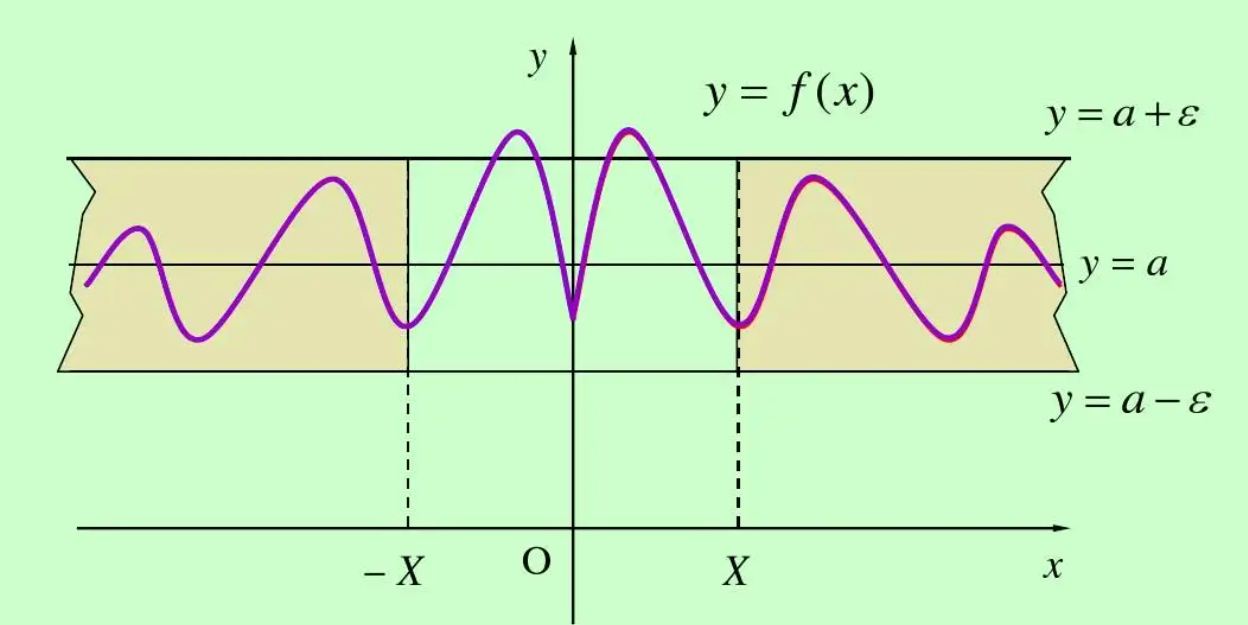
\includegraphics[width=0.7\textwidth]{figures/limfun}
		\caption{函数极限定义}\label{limfun}
	\end{figure}
	
	
	\subsection{自变量$x$趋于有限值时函数的极限}
	数列极限只研究了当自变量趋于无穷大时的极限,但是对于函数极限来说,考虑到其“连续型”的特征,我们还需要研究自变量$x$趋于有限值$x_0$时的函数极限。例如,函数连续性和导数都是用某一点处的函数极限来定义的。
	
	$x$趋于$x_0$也包括三种情形:
	\begin{itemize}
		\item 在数轴上$x$从$x_0$右侧趋近于$x_0$,记作$x \to x_{0}^{+}$;
		\item 在数轴上$x$从$x_0$左侧趋近于$x_0$,记作$x \to x_{0}^{-}$;
		\item 在数轴上$x$从$x_0$左右两侧趋近于$x_0$,记作$x \to x_{0}$.
	\end{itemize}

	下面主要讨论$x \to x_{0}$时的情况.
	
	我们需要关心当$x \to x_{0}$时,函数值$f(x)$的变化趋势.类似地,我们给出以下定义:
	\begin{definition}[\textbf{$x\to x_0$时的函数极限}]
		设函数$f(x)$在点$x_0$的某一去心邻域内有定义.如果存在常数a,对于任意给定的正数$\varepsilon$,总存在正数$\delta$,使得当x满足$0<\left|x-x_0\right|<\delta$时,
		\[
		\left|f(x)-a\right|<\varepsilon,
		\]
		那么常数a就叫做函数$f(x)$当$x\to x_0$时的$f(x)$的\textbf{极限},记作
		\[
		\lim_{x\to x_0}f(x)=a.
		\]\\
		此时,称当$x\to x_0$时,$f(x)$\textbf{极限存在}.
		
		$\star$注意x是在$x_0$的\textbf{去心邻域},不能取到$x_0$这个点.
		\
		
	\end{definition}
	
	\begin{example}
			\[
		f(x) =
		\begin{cases}
			x^2 &  x\ne 0 ,\\
			1 &  x =0 .
		\end{cases}
		\]
		在$x=0$处的函数极限为0,而不是1.
	\end{example}
	
	类似地,可以定义当$x \to x_{0}^{+}$或$x \to x_{0}^{-}$时函数的极限,分别叫做\textbf{左极限}或\textbf{右极限}.
	
	我们有如下结论:
	\[
	\lim_{x\to x_0}f(x)=a \text{当且仅当} \lim_{x\to x_{0}^{+}}f(x)=\lim_{x\to x_{0}^{-}}f(x)=a.
	\]
	也就是说,$f(x)$极限存在的充要条件是$f(x)$的左右极限都存在且相等.这个结论可以作为判断函数极限是否存在的一个方法.
	\begin{example}
		判断函数$f(x)=\frac{\left|x\right|}{x},$当$x\to 0$时极限是否存在.
	\end{example}
	\begin{solution}
		由于
		\[
		\lim_{x\to 0^-}=\lim_{x\to 0^-}\frac{-x}{x}=-1,
		\]\[
		\lim_{x\to 0^+}=\lim_{x\to 0^+}\frac{x}{x}=1,
		\]
		故左极限不等于右极限,极限不存在.
	\end{solution}

	\begin{example}
		判断函数$f(x)=e^\frac{1}{x-2}$,当$x\to 2$时极限是否存在.
	\end{example}
	\begin{solution}
		由于\[
		\lim_{x\to 2^-}f(x)=0,
		\]\[
		\lim_{x\to 2^+}f(x)=+\infty,
		\]
		故左右极限不相等,极限不存在.
	\end{solution}
	
	
	\subsection{函数极限的归并原理}
	上一节我们已经了解了数列极限的归并原理,它是连接数列和其子列极限的桥梁.下面我们将介绍函数极限的归并原理,它是连接函数极限和数列极限的桥梁.被称为\textbf{Heine定理}.
	\begin{theorem}[\textbf{Heine定理}]
		函数$f$在$x_0$处有极限a的充分必要条件是:对于任意一个收敛于$x_0$的数列${x_n}(x_n\neq x_0)$,数列${f(x_n)}$有极限a.\\
		$\star$注意$x_n\neq x_0$.
	\end{theorem}
	Heine定理有以下两个主要作用:
		\begin{itemize}
		\item 判断函数极限是否存在;
		\item 将未知的函数问题转化为已知的数列问题.
	\end{itemize}
	下面这个例题将展示Heine定理如何处理判断极限是否存在的问题.
	\begin{example}
		设$f(x)=\sin\frac{1}{x}$,证明当$x\to 0$时极限不存在.
	\end{example}
	\begin{proof}
		设$x_n=(2n\pi + \frac{\pi}{2})^{-1},y_n=(2n\pi - \frac{\pi}{2})^{-1}$,
		
		则$x_n\to 0,y_n\to 0,x_n,y_n\in ,\mathbb{R}\setminus \{0\}$,
		
		且对任意正整数$n$都有$f(x_n)=1,f(y_n)=-1,f(x_n)\ne f(y_n)$.
		
		故$f(x)$极限不存在.
	\end{proof}
	关于反三角函数,还有两个重要极限:
	\begin{example}
		$\lim\limits_{x\to +\infty} \arctan x=\frac{\pi}{2}$
		
		$\lim\limits_{x\to -\infty} \arctan x=-\frac{\pi}{2}$
	\end{example}
	
	\section{函数极限的性质}
	函数极限与数列极限有很多相似的性质,很多性质可以利用上文提到的Heine定理转化为数列极限来证明.
	
	\begin{theorem}[\textbf{唯一性}]
		设$\lim\limits_{x\to x_0}f(x)=a$,则当$x\to x_0$时,$f(x)$的极限是唯一的.
	\end{theorem}
	
	\begin{theorem}[\textbf{局部有界性}]
		设$\lim\limits_{x\to x_0}f(x)=a$,则$f$在$x_0$处是\textbf{局部有界的},即存在$M>0$与$\delta >0$,使得对于任意的$x\in \left(x_0-\delta,x_0+\delta \right)\backslash \{x_0\}$,都有$\left|f(x)\right| \le M$.
	\end{theorem}

	\begin{theorem}[\textbf{局部保号性}]
		设$\lim\limits_{x\to x_0}f(x)=a$,$\lim\limits_{x\to x_0}g(x)=b$,若$a\ne 0$,则存在$\delta >0$,使得对于任意的$x\in \left(x_0-\delta,x_0+\delta \right)\backslash \{x_0\},f(x)$都与$a$同号.特别若$a>0\left(a<0 \right),$则存在$\delta >0,$使得任意$x\in \left(x_0-\delta,x_0+\delta \right)\backslash \{x_0\}$,恒有$f(x)\ge q \ge 0\left(f(x) \le q \le 0\right)$.
	\end{theorem}

	\begin{theorem}[\textbf{局部保序性}]
		设$\lim\limits_{x\to x_0}f(x)=a$,$\lim\limits_{x\to x_0}g(x)=b$,若存在$\delta>0,$使得对于任意的$x\in \left(x_0-\delta,x_0+\delta \right)\backslash \{x_0\}$,恒有$f(x)\le g(x)$,则$a\le b$.
	\end{theorem}	
	以上三个性质都是\textbf{局部}的性质,反映函数在某一个点附近的性质.
	
	\begin{theorem}[\textbf{夹逼性}]
		设$\lim\limits_{x\to x_0}f(x)=a$,$\lim\limits_{x\to x_0}g(x)=b$,若存在$\delta>0,$使得对于任意的$x\in \left(x_0-\delta,x_0+\delta \right)\backslash \{x_0\}$,恒有$f(x) \le \phi(x) \le g(x),$且$a=b$,则$\lim\limits_{x\to x_0}\phi (x)=a$.
	\end{theorem}
	$\star$ 夹逼性定理常用于计算某些函数极限.
	\begin{example}
		计算$\lim\limits_{x\to 0}x\left[\frac{1}{x}\right]=1$.
	\end{example}
	\begin{solution}
		由于$x(\frac{1}{x}-1)\le x\left[\frac{1}{x}\right]\le x\cdot \frac{1}{x}$,
		
		且$\lim\limits_{x\to 0}x(\frac{1}{x}-1)=1,\lim\limits_{x\to 0}x\cdot \frac{1}{x}=1$,
		
		故$\lim\limits_{x\to 0}x\left[\frac{1}{x}\right]=1$.
	\end{solution}
	
	\begin{theorem}[\textbf{有理运算法则}]
		设$\lim\limits_{x\to x_0}f(x)=a$,$\lim\limits_{x\to x_0}g(x)=b$,则
		\begin{enumerate}
			\item 
			\[\lim_{x\to x_0}(f(x)\pm g(x))=\lim_{x\to x_0}f(x) \pm \lim_{x\to x_0}g(x)=a\pm b;
			\]
			\item 
			\[\lim_{x\to x_0}f(x)g(x)=\lim_{x\to x_0}f(x) \lim_{x\to x_0}g(x)=ab;
			\]
			\item 
			\[\lim_{x\to x_0}\frac{f(x)}{g(x)}=\frac{\lim\limits_{x\to x_0}f(x)}{\lim\limits_{x\to x_0}g(x)}=\frac{a}{b},\text{其中}b \ne 0.
			\]
		\end{enumerate}
	\end{theorem}
	以上几个定理同样适用于$x\to \infty,x \to \pm\infty, x\to x_{0}^{\pm}$等情形.
	\begin{example}
		若$\lim\limits_{x\to x_0}f(x)$和$\lim\limits_{x\to x_0}(f(x)-g(x))$都存在,则$\lim\limits_{x\to x_0}g(x)$也存在.
	\end{example}
	
	\begin{theorem}[\textbf{复合函数极限运算法则}]
		设$y=(f\circ g)(x)=f(g(x))$是由$y=f(u)$与$u=g(x)$复合而成,复合函数$f\circ  g$定义在$x_0$的某去心邻域$\overset{\circ}{U}(x_0)$中.若$\lim\limits_{x\to x_0}g(x)=u_0,\lim\limits_{u\to u_0}f(u)=a,$并且存在$\delta _0>0$,使得对于任意的$x\in \overset{\circ}{U}(x_0,\delta_0),$恒有$g(x)\ne u_0$,则
		\[\lim_{x\to x_0}f(g(x))=a=\lim_{u\to u_0}f(u).
		\]
	\end{theorem}	
	此定理给出了求复合函数极限时,运用变量替换法的条件.复合函数极限运算法则可以应用于下一个部分,之后将给出例题.	
		

	\section{两个重要极限}
	下面介绍两个非常重要且常用的极限,它们不仅可以用来求复杂函数的极限,也是推导导数公式的基础.
	\begin{enumerate}
		\item 	$\lim\limits_{x\to 0}\frac{\sin x}{x}=1$;
		\item 	$\lim\limits_{x\to \infty}(1+\frac{1}{x})^x=e$.
	\end{enumerate}
	这两个极限的证明见教材,请同学们尽量掌握.
	
	\begin{example}
		求$\lim\limits_{x\to 0}\frac{\sin2x}{x}.$
	\end{example}
	\begin{solution}
		\[
		\lim\limits_{x\to 0}\frac{\sin2x}{x}=\lim\limits_{x\to 0}\frac{\sin2x}{2x}\cdot 2=2\].
	\end{solution}

	\begin{example}
		求$\lim\limits_{x\to 0}x\cot 2x$.
	\end{example}
	\begin{solution}
		\[
		\lim\limits_{x\to 0}x\cot 2x=\lim\limits_{x\to 0}x\cdot\frac{\cos 2x}{\sin 2x}=\lim\limits_{x\to 0}\frac{2x}{\sin2x}\cdot\frac{\cos2x}{2}=\frac{1}{2}.
		\]
	\end{solution}

	\begin{example}
		求$\lim\limits_{x\to 0}(1-3x)^{\frac{2}{x}}.$
	\end{example}
	\begin{solution}
		\[
		\lim\limits_{x\to 0}(1-3x)^{\frac{2}{x}}=\lim\limits_{x\to 0}(1+(-3x))^{-\frac{1}{3x} \cdot (-3x) \cdot \frac{2}{x}}=e^{\lim\limits_{x\to 0}-\frac{6x}{x}}=e^{-6}. 
		\]
	\end{solution}

	\begin{example}
		求$\lim\limits_{x\to 0}(\cos x+x\sin x)^{\frac{1}{x^2}}.$
	\end{example}
	\begin{solution}
		\begin{align*}
		\lim\limits_{x\to 0}(\cos x+x\sin x)^{\frac{1}{x^2}}&=\lim\limits_{x\to 0}(1+\cos x+x\sin x-1)^{\frac{1}{x^2}}\\
		& = \lim\limits_{x\to 0}(1+\cos x+x\sin x-1)^{\frac{1}{\cos x+x\sin x-1}\cdot \frac{\cos x+x\sin x-1}{x^2}}\\
		& = {\rm e}^{\lim\limits_{x\to 0}\frac{\cos x+x\sin x-1}{x^2}}\\
		& = {\rm e}^{\lim\limits_{x\to 0}\frac{\cos x-1}{x^2}+\frac{\sin x}{x}}\\
		& = {\rm e}^{-\frac{1}{2}+ 1}\\
		& = {\rm e}^{\frac{1}{2}}.
		\end{align*}
	\end{solution}
	
	\section{函数极限的存在准则}
	与数列极限类似,下面将介绍函数极限的单调有界准则和Cauchy收敛原理.
	\begin{theorem}[\textbf{单调有界准则}]
		
			\begin{enumerate}
				\item 	设函数$f$在区间$\left[a,+\infty \right) \left(a\in \mathbb{R} \right)$上单调增或减,有上或下界,则$\lim\limits_{x\to x_0}f(x)$存在;
				\item 	设函数$f$是区间$I$上的单调函数,则$f$在$I$内每一点的单侧极限存在.
			\end{enumerate}
	\end{theorem}

	\begin{theorem}[\textbf{Cauchy收敛原理}]
		设$f:\overset{\circ}{U}(x_0)\to \mathbb{R}$是任一函数,则$\lim\limits_{x\to x_0}f(x)$存在的充要条件是:对于任意$\varepsilon>0$,存在$\delta>0$,使得对于任意的$x_1,x_2\in \overset{\circ}{U}(x_0,\delta)$,恒有
		\[
		\left|f(x_1)-f(x_2)\right|<\varepsilon,
		\]
		其中$\overset{\circ}{U}(x_0,\delta)\subseteq\overset{\circ}{U}(x_0)$.
	\end{theorem}
	几何直观上来看,若$\lim\limits_{x\to x_0}f(x)$存在,则当$x\to x_0$时,$f$的振幅趋于零.这就为我们提供一种证明函数极限不存在的新思路.
	
	例如,函数$f(x)=\sin\frac{1}{x}$的图像(如图\ref{sinfun})在$x=0$附近不停振荡,不满足Cauchy收敛原理,因此它在$x=0$处的极限不存在.
	\begin{figure}[H]
		\centering
		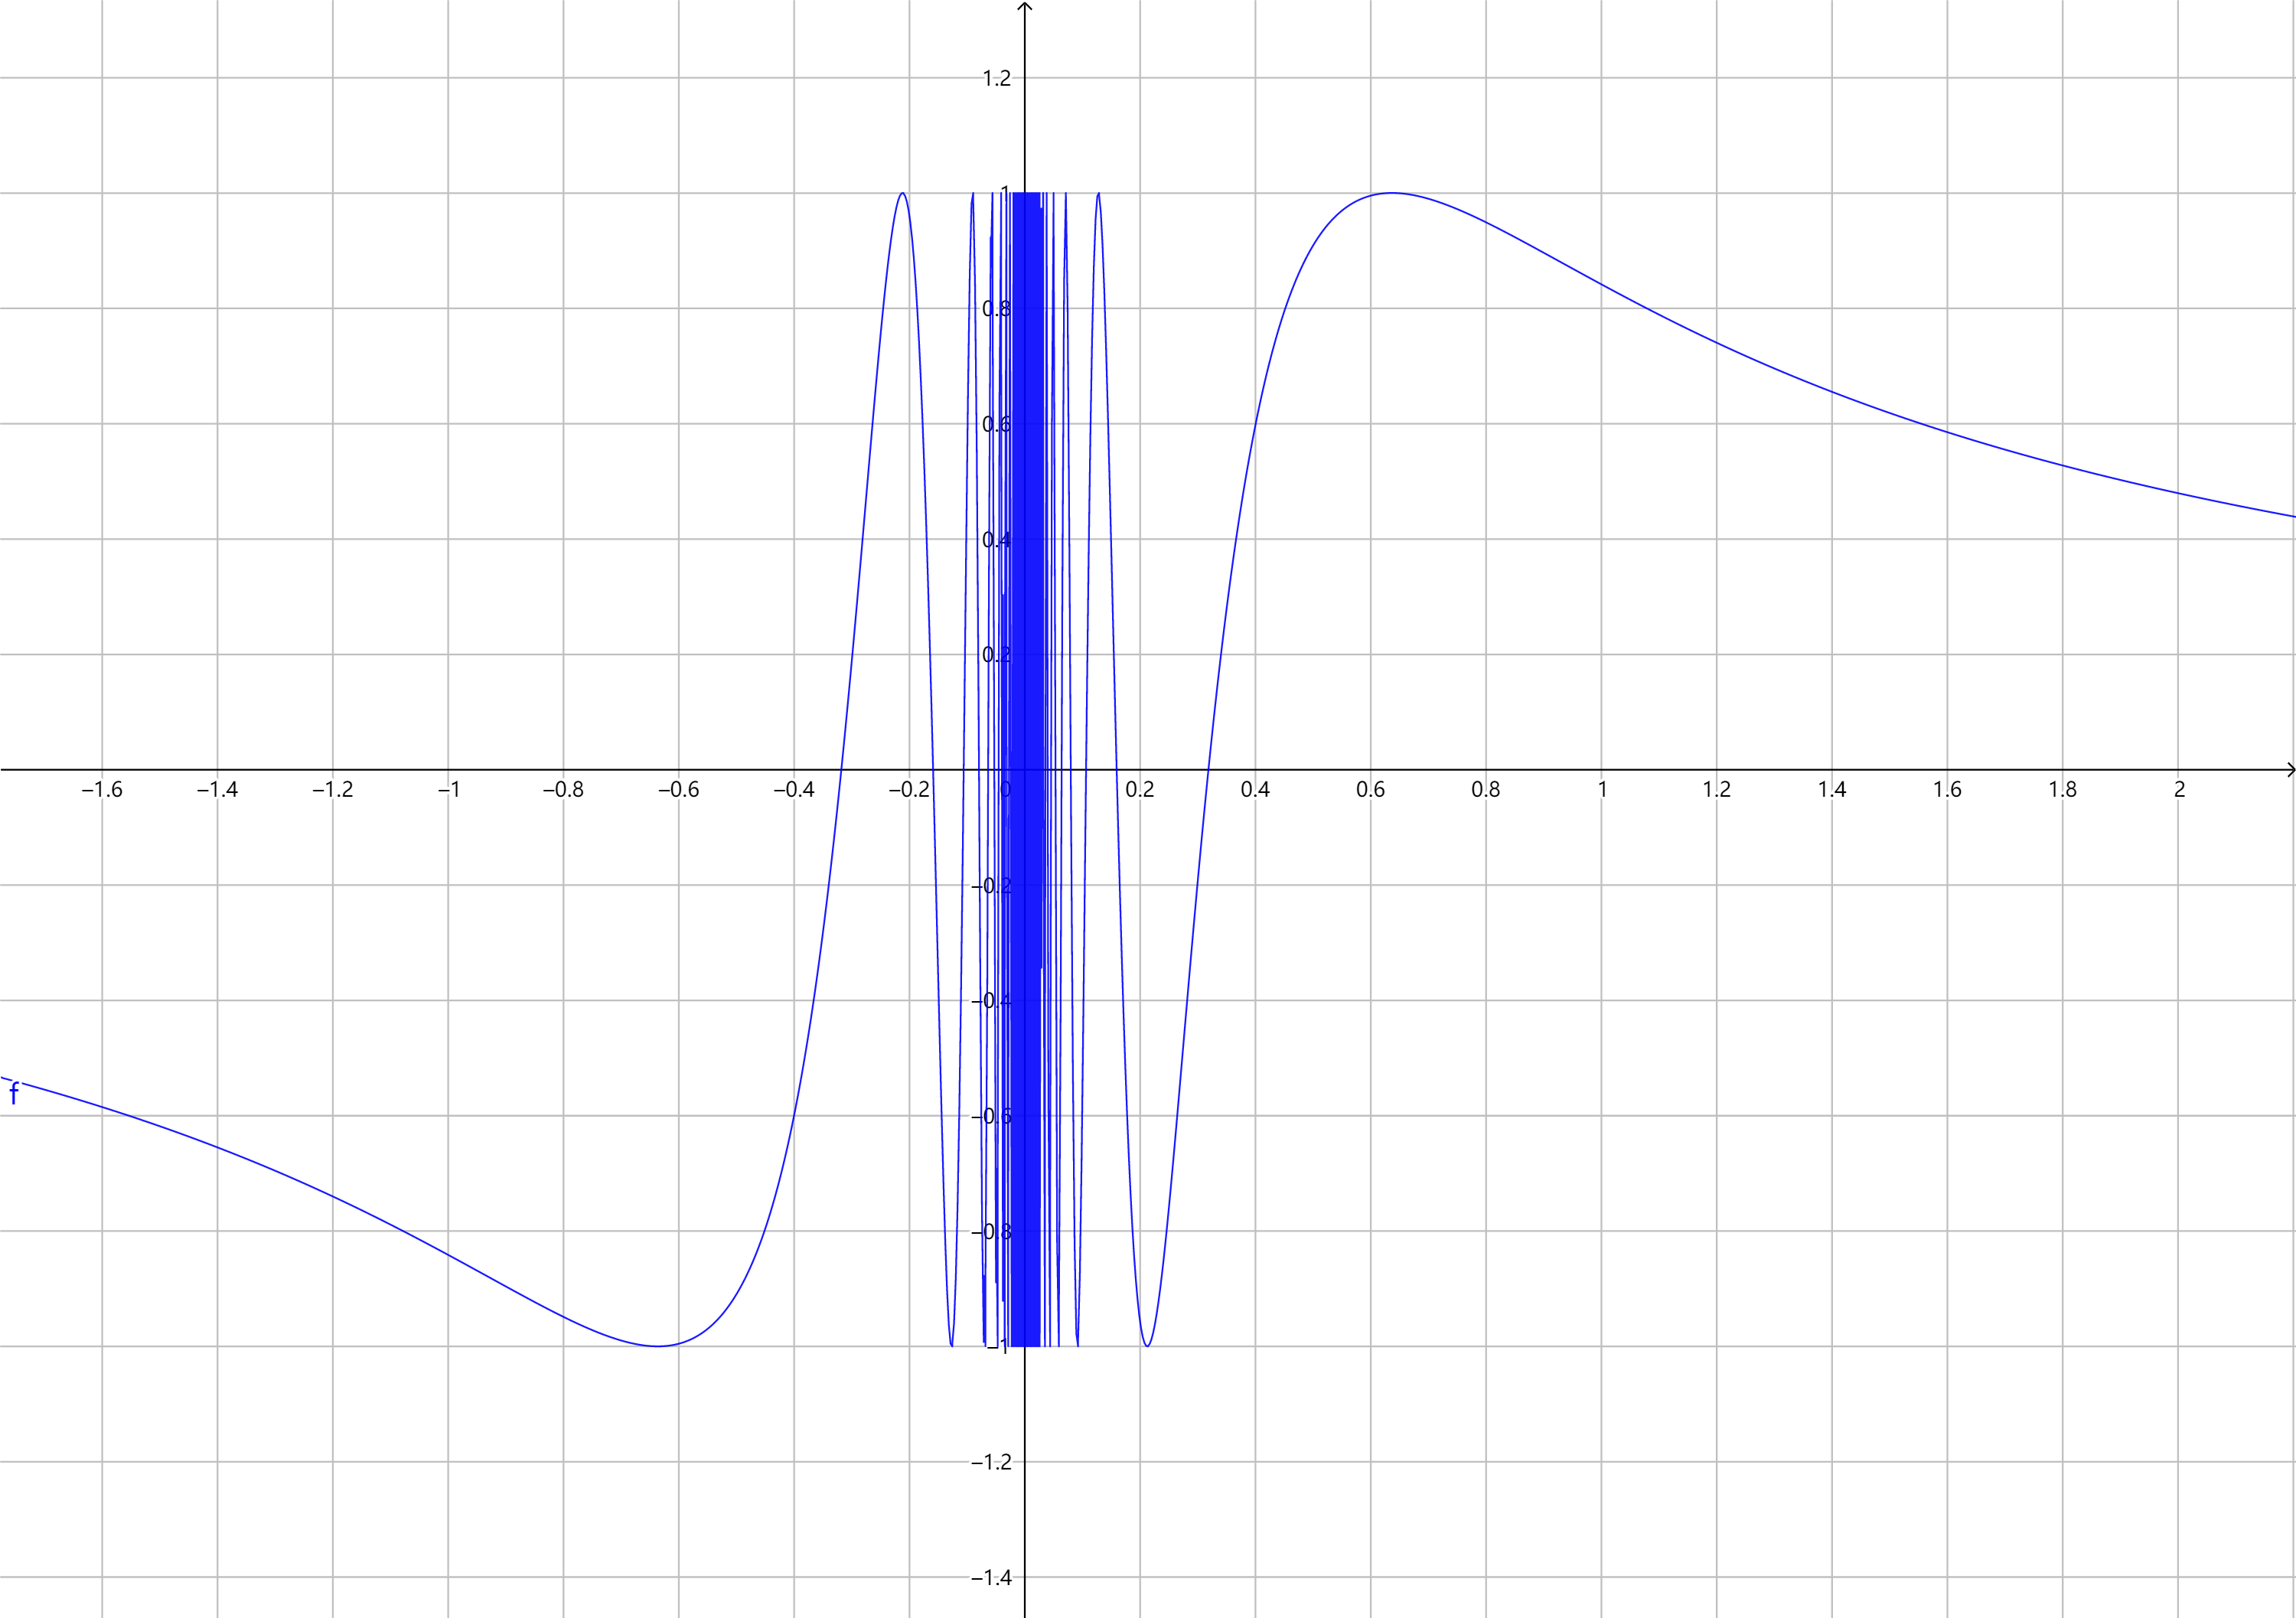
\includegraphics[width=0.5\textwidth]{figures/sinfun}
		\caption{$f(x)=\sin\frac{1}{x}$图像}\label{sinfun}
	\end{figure}

% \chapter{占位章}
\chapter{无穷小量与无穷大量}

本节课主要介绍无穷小量和无穷大量的概念。无穷小量在求函数极限的过程中有重要作用,无穷小量也广泛应用于函数(数列)极限阶的估计。
	
	本节课的主要内容包括:
	\begin{enumerate}
		\item 无穷小量的概念与性质;
		\item 无穷小在求函数极限过程中的应用;
		\item 无穷大量。
	\end{enumerate}

	\section{无穷小量的概念与性质}
	
	\begin{definition}[\textbf{无穷小量}]
		当$x\to x_0\left(x\to \infty\right)$时,以零为极限的函数$\alpha(x)$称为当$x\to x_0\left(x\to \infty\right)$时的\textbf{无穷小量},简称为\textbf{无穷小}.
	\end{definition}

	例如,当$x\to 0$时,$x^2,\sin x,\tan x$都是无穷小;当$x\to \infty \text{时},\frac{1}{x},\frac{\sin x}{x}$都是无穷小.
	
	同时,以零为极限的数列也是无穷小($n\to \infty$).
	
	$\star$注意,无穷小量是以零为极限的\textbf{变量},而不是一个绝对值很小的常数.
	
	下面介绍三个无穷小量的定理.
	\begin{theorem}
		$\lim\limits_{}f(x)=a \text{当且仅当}f(x)=a+\alpha(x)$,其中$\alpha(x)$是无穷小.
	\end{theorem}

	\begin{theorem}
		在自变量有相同变化趋势的条件下。有
		\begin{enumerate}
			\item 有限个无穷小量的代数和是无穷小量;
			\item 有限个无穷小量的乘积是无穷小量.
		\end{enumerate}
	\end{theorem}

	\begin{theorem}
		\label{the3}
		设$\alpha(x)$是当$x\to x_0$时的无穷小,$f$是在$x_0$处局部有界的函数,则$\alpha (x)f(x)$是当$x\to x_0$时的无穷小.
	\end{theorem}
	
	定理\ref{the3}也就是说:\textbf{无穷小与有界函数的积还是无穷小}.
	
	\begin{example}
		求极限$\lim\limits_{x\to 0}x\sin\frac{1}{x}$.
	\end{example}

	\begin{solution}
		由于当$x\to 0$时,$x$是无穷小,并且当$x\ne 0$时,$\left|\sin\frac{1}{x}\right| \le 1$,故$\sin\frac{1}{x}$在$x=0$的任一去心邻域内是有界函数,所以由定理\ref{the3},
		\[
		\lim_{x\to 0}x\sin\frac{1}{x}=0.
		\]
	\end{solution}

	\section{无穷小的比较}
	首先,我们观察以下三个极限:
	\begin{enumerate}
		\item $\lim\limits_{x\to 0}\frac{x^2}{x}=0$;
		\item $\lim\limits_{x\to 0}\frac{2x}{x}=2$;
		\item $\lim\limits_{x\to 0}\frac{\sin{x}}{x}=1$.
	\end{enumerate}

	它们的分子分母都是无穷小量,但是比值的极限却各不相同.我们会想为什么不同无穷小比值的极限存在差异?是否可以通过某种方法来比较两个无穷小量“谁更小”.
	
	这里,我们引入无穷小阶的概念来解决这个问题.
	\begin{definition}
		设$\alpha (x)\text{与} \beta (x)$是自变量$x$有相同变化趋势的无穷小,且$\beta (x)\ne 0.$
		\begin{enumerate}
			\item 
			若$\lim\limits_{}\frac{\alpha(x)}{\beta (x)}=0$,则称$\alpha(x)$是$\beta(x)$的\textbf{高阶无穷小},或称$\beta(x)$是$\alpha(x)$的\textbf{低阶无穷小},记作$\alpha(x)=o(\beta(x))$.特别,一个无穷小$\alpha(x)$可记作$o(1)$.
			\item 
			若$\lim\limits_{}\frac{\alpha(x)}{\beta (x)}=c$,且$c\ne 0$为常数,则称$\alpha(x)$与$\beta(x)$是\textbf{同阶无穷小}.
			\item 
			若$\lim\limits_{}\frac{\alpha(x)}{\beta (x)}=1$,则称$\alpha(x)$与$\beta(x)$是\textbf{等价无穷小},记作$\alpha (x)\sim\beta(x)$.
			\item 
			若$\lim\limits_{}\frac{\alpha(x)}{(\beta (x))^k}=c$,其中$c\ne 0$为常数,$k>0$,则称$\alpha(x)$是\textbf{关于$\beta(x)$的$k$阶无穷小}.特别地,若取$\beta(x)=x-x_0$,若$\lim\limits_{x\to x_0}\frac{\alpha(x)}{(x-x_0)^k}=c$,则称$\alpha (x)$是当$x\to x_0$时的\textbf{$k$阶无穷小}.
		\end{enumerate}
	\end{definition}
	例如,当$x\to 0$时,
	
	$x^3+2x^2$与$2x^2$是等价无穷小,即$x^3+2x^2 \sim 2x^2$;
	
	$\sin{x}$与$x$是等价无穷小,即$\sin{x}\sim x$.
	
	\begin{theorem}
		设$\alpha(x)$与$\beta(x)$是在自变量同一变化趋势下的无穷小,且$\alpha(x)\sim \beta(x)$,则$\alpha(x)=\beta(x)+o(\beta(x))$或$\beta(x)=\alpha(x)+o(\alpha(x)).$
	\end{theorem}
	下面介绍几个常用的等价无穷小:
	
	当$x\to 0$时,
	\begin{enumerate}
		\item $\sin{x}\sim x$;
		\item $\tan{x}\sim x$;
		\item $\arctan{x}\sim x$;
		\item $1-\cos{x}\sim \frac{x^2}{2}$;
		\item $e^x-1\sim x$;
		\item $\ln{(1+x)}\sim x$;
		\item $(1+x)^{\alpha }-1\sim \alpha x$.
	\end{enumerate}
	\textbf{$\star$以上式子非常重要,请同学们务必掌握.}

	\section{无穷小的等价替换}
	\begin{theorem}[无穷小等价代换定理]
		设$\alpha(x)$与$\beta(x)$,$\tilde{\alpha}(x)$与$\tilde{\beta}(x)$都是在自变量同一变化趋势下的无穷小.若$\alpha(x)\sim \beta(x)$,$\tilde{\alpha}(x)\sim \tilde{\beta}(x)$,并且$\lim\limits_{}\frac{\tilde{\alpha}(x)}{\tilde{\beta}(x)}$存在,则$\lim\limits_{}\frac{\alpha(x)}{\beta(x)}$也存在,并且
			\[
			\lim\frac{\alpha(x)}{\beta(x)}=\lim\frac{\tilde{\alpha}(x)}{\tilde{\beta}(x)}.
			\]
	\end{theorem}

	这是一个非常重要的定理,经常用于极限的计算.它可以将$\frac{0}{0}$型不定式极限的分子分母用更简单的等价无穷小代换,便于计算.下面给出几个例子.
	
	\begin{example}
		求$\lim\limits_{x\to 0}\frac{\sqrt[3]{1+2x^2}-1}{\arcsin\frac{x}{2}\arctan\frac{x}{3}}$.
	\end{example}
	\begin{solution}
		由于当$x\to 0$时,
		\[
		(1+2x^2)^{\frac{1}{3} }-1\sim \frac{2}{3}x^2,
		\]
		\[
		\arcsin\frac{x}{2}\sim \frac{x}{2},
		\]
		\[
		\arctan\frac{x}{3}\sim \frac{x}{3},
		\]
		所以,
		\[
		\lim_{x\to 0}\frac{\sqrt[3]{1+2x^2}-1}{\arcsin\frac{x}{2}\arctan\frac{x}{3}}=\lim_{x\to 0}\frac{\frac{2}{3}x^2}{\frac{x}{2}\frac{x}{3}}=4.
		\]
	\end{solution}

	\begin{example}
		求$\lim\limits_{x\to 0}\frac{(1+x)^{\sqrt{2} }-1 }{x} .$
	\end{example}
	\begin{solution}
		\[
		\lim\limits_{x\to 0}\frac{(1+x)^{\sqrt{2} }-1 }{x}=\lim_{x\to 0}\frac{\sqrt{2}x}{x}=\sqrt{2}.
		\]
	\end{solution}

	\section{无穷大量}
	我们已经介绍过无穷小量,无穷大量与无穷小量相似,只是无穷大量的变化状态正好相反.
	首先,我们来定义无穷大量.
	
	\begin{definition}[\textbf{无穷大量}]
		设$f:\overset{\circ}{U}(x_0)\to \mathbb{R}$是一个函数,若$\lim\limits_{x\to x_0}f(x)=\infty$,则称函数$f(x)$是当$x\to x_0$时的\textbf{无穷大量}.
	\end{definition}
	\begin{itemize}
		\item 若$\lim\limits_{x\to x_0}f(x)=+\infty$,则称$f(x)$是当$x\to x_0$时的\textbf{正无穷大}.
		\item 若$\lim\limits_{x\to x_0}f(x)=-\infty$,则称$f(x)$是当$x\to x_0$时的\textbf{负无穷大}.
	\end{itemize}
	
	无穷大量和无穷小量之间有如下关系:
	\begin{theorem}
		\begin{enumerate}
			\item 若$f(x)$是无穷小量,且$f(x)\ne 0$,则$\frac{1}{f(x)}$是无穷大量;
			\item 若$f(x)$是无穷大量,则$\frac{1}{f(x)}$是无穷小量.
		\end{enumerate}
	\end{theorem}

	与无穷小量相似,无穷大量有以下运算性质:
	\begin{theorem}
	\begin{enumerate}
		\item 有限个无穷大量的乘积是无穷大量.
		\item 无穷大量与有界量之和是无穷大量.
	\end{enumerate}
	\end{theorem}

\chapter{连续函数}

本节课主要介绍函数的连续性.连续函数有很多好的性质,在今后微分和积分的学习中有重要作用.我们已经学习过函数极限,函数连续性也是在函数极限的基础上定义的.

本节课主要内容包括:
\begin{enumerate}
	\item 函数连续性的概念;
	\item 连续函数的运算;
	\item 闭区间连续函数的性质;
	\item 函数的一致连续性.
\end{enumerate}

\section{函数的连续性概念与间断点的分类}
\subsection{函数的连续性概念}
我们见过的很多初等函数,例如$y=x^2,y=\sin x,y=\sqrt{x},y=\left|x\right|$等等,在定义域内都是连续函数;同时,我们也遇到过一些不连续的函数,例如:

Dirichlet函数:
\[
	f(x) =
	\begin{cases}
		0 & x \text{为无理数} , \\
		1 & x \text{为有理数} .
	\end{cases}
\]

取整函数$f(x)=[x]$,如图\ref{roundfun}.
\begin{figure}[H]
	\centering
	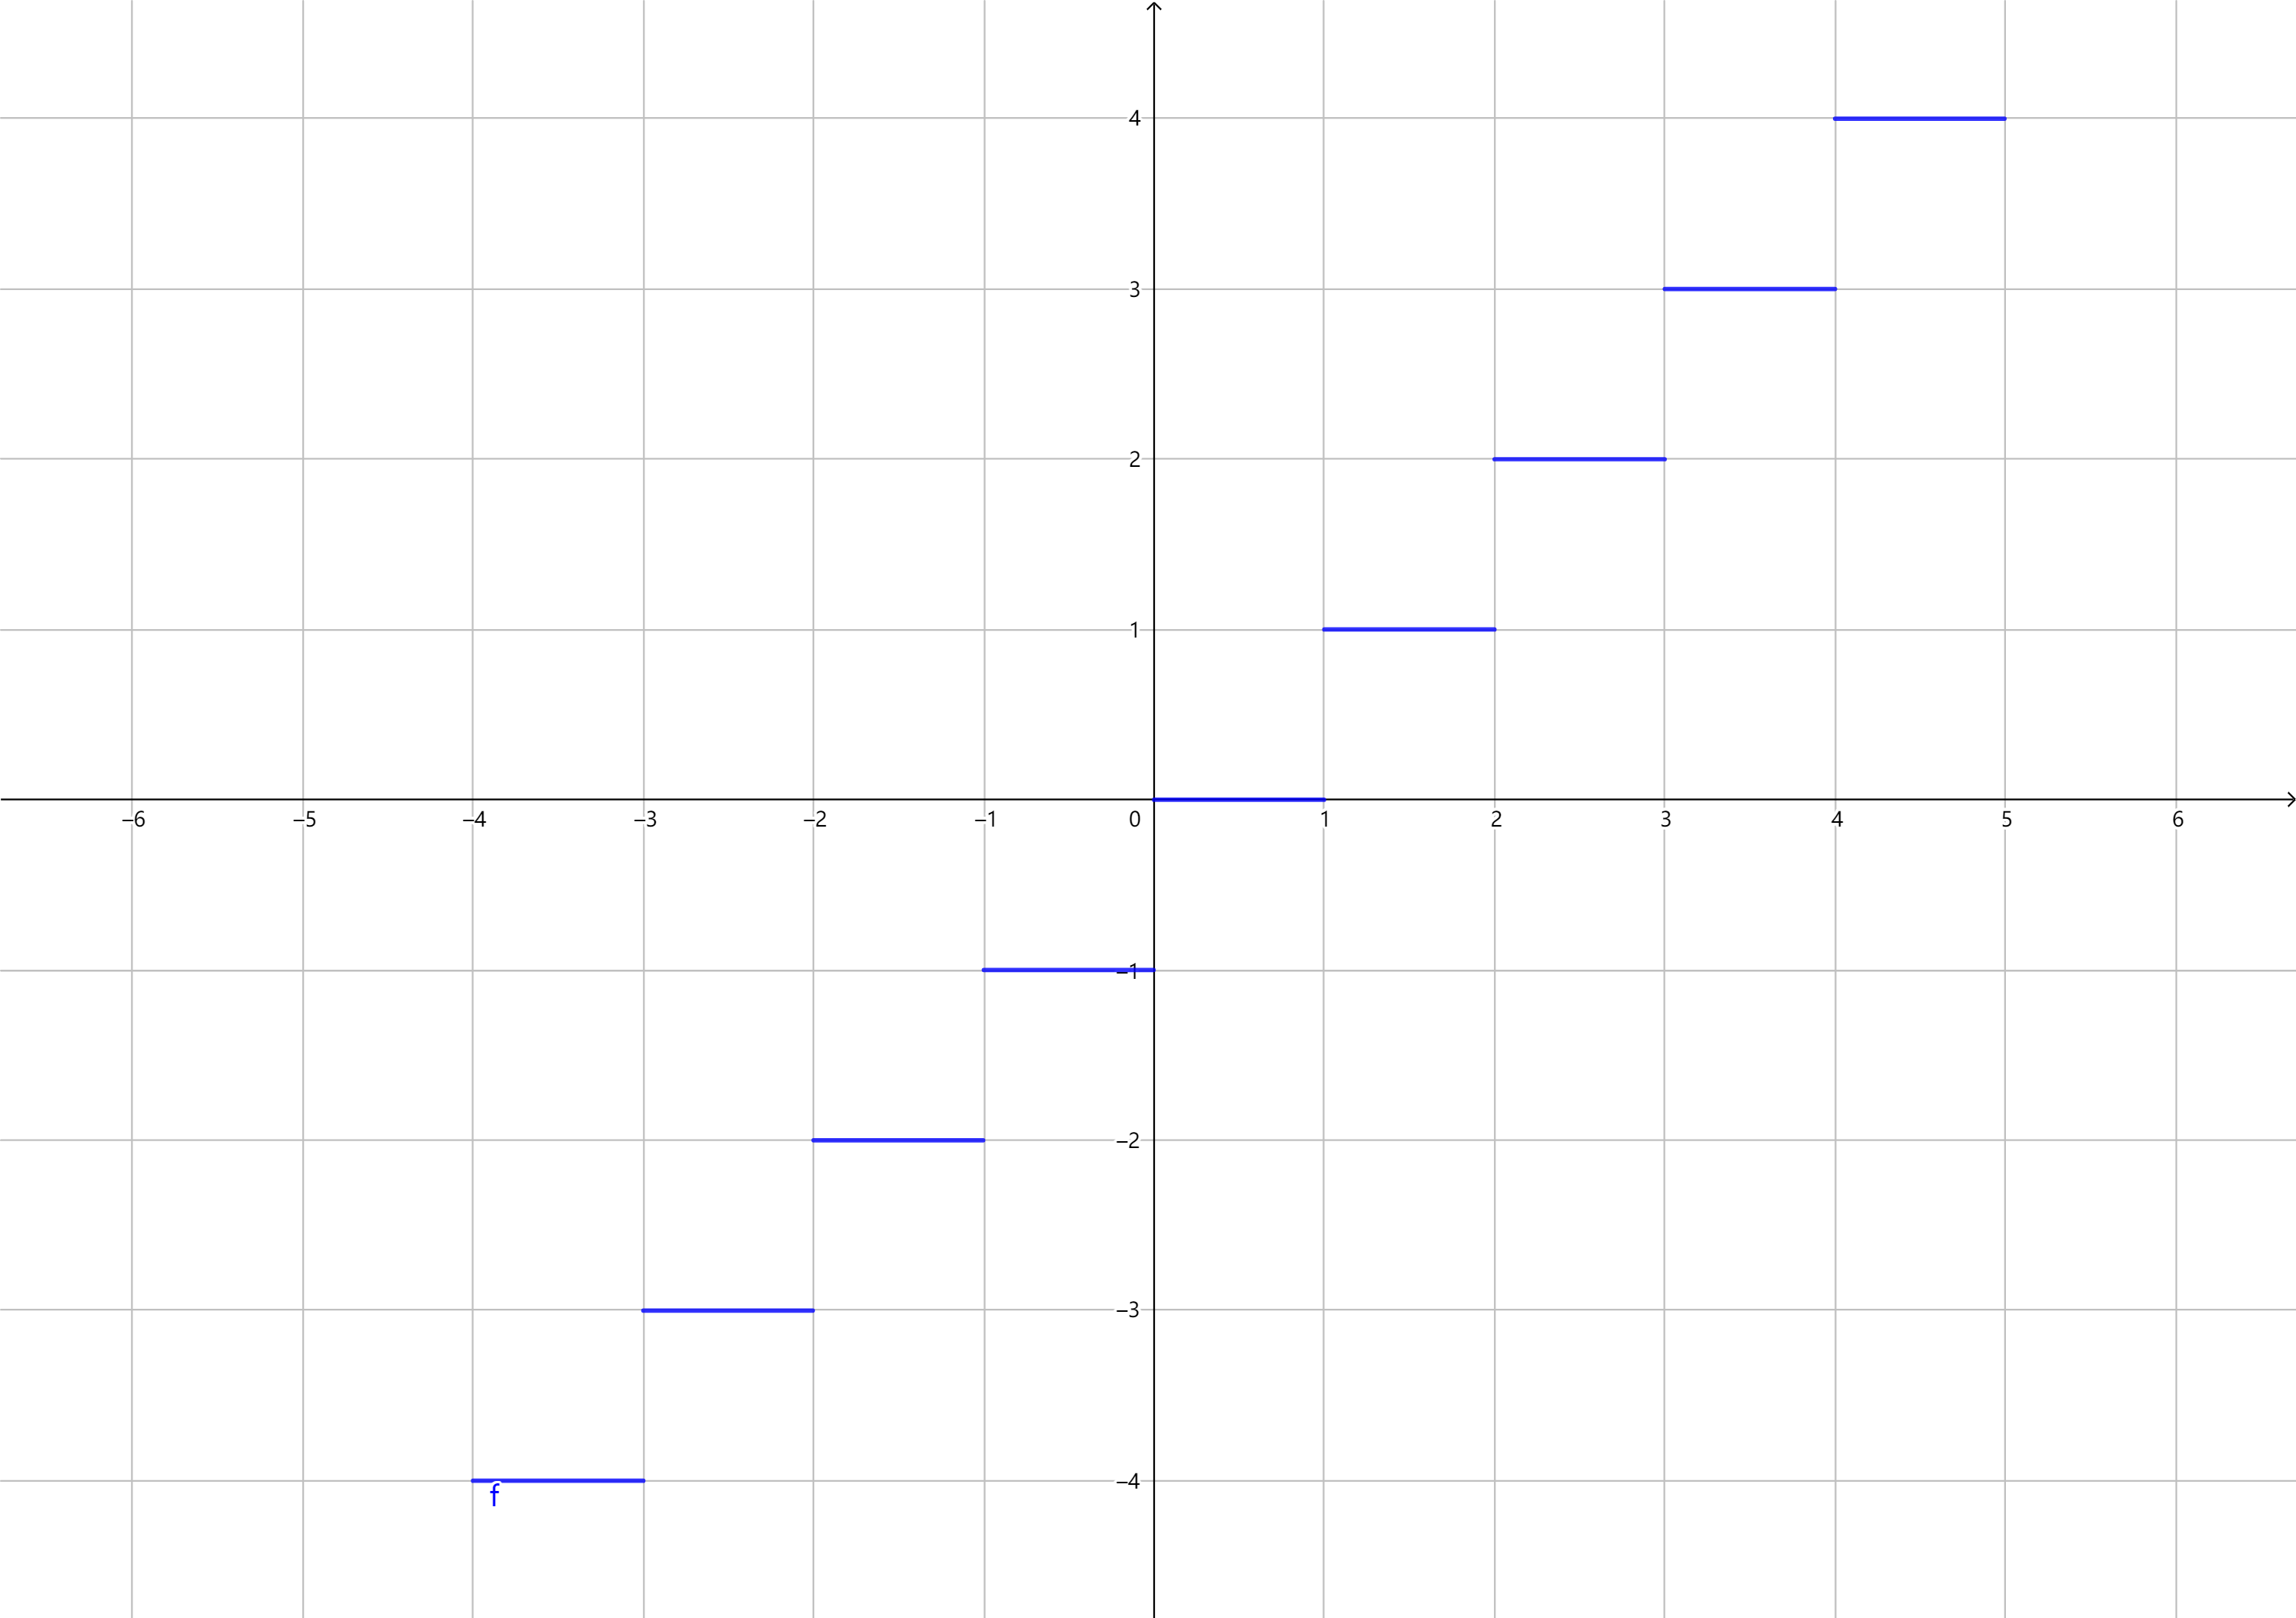
\includegraphics[width=0.6\textwidth]{figures/roundfun}
	\caption{$f(x)=[x]$图像}\label{roundfun}
\end{figure}

由这几个例子,我们可以明显看出连续函数和不连续函数的区别.连续函数的自变量改变量$\Delta x\to 0$时,因变量的改变量$\Delta y\to 0$.而不连续函数的自变量改变量$\Delta x\to 0$时,函数值可能发生跳跃,函数值的极限不趋于0.基于此,我们可以这样来定义连续函数:

\begin{definition}[\textbf{连续函数}]
	设函数f定义在$\left[a,b\right]$上,对于任意一点$x_{0}\in \left(a,b\right)$,若对于任意给定的$\epsilon>0$,存在$\delta>0$,使得对于任意满足$\left|x-x_0\right|<\delta$的x,有
	\[
		\left|f(x)-f(x_0)\right|<\epsilon
	\]
	那么就称函数f在$x_0$处连续,如果f在$\left[a,b\right]$中每一点都连续,那么就称函数f在区间$\left[a,b\right]$上连续.
\end{definition}

我们记在区间$I$上连续函数的全体构成的集合为$C(I)$.

类似左极限和右极限,我们也可以来定义左连续和右连续.
\begin{enumerate}
	\item 左连续:$\lim\limits_{x\to x_{0}^{-}}f(x)=f(x_0)$;
	\item 右连续:$\lim\limits_{x\to x_{0}^{+}}f(x)=f(x_0)$;
\end{enumerate}

\begin{theorem}
	函数在某一点处连续当且仅当函数在这一点处既左连续又右连续.
\end{theorem}

\subsection{间断点的分类}
我们已经讨论了连续函数,下面还需要讨论一个函数不连续的情况.

如果函数$f$在$x_0$处不连续,那么这个函数就不是连续函数,所以我们要研究不连续点的情况.

\begin{definition}[\textbf{函数的间断点}]
	设函数$f$在$x_0$的某一单侧邻域内有定义,若$f$在$x_0$不连续,那么称$x_0$是$f$的一个间断点.
\end{definition}
根据函数间断点的特征,有以下几个分类:

\begin{enumerate}
	\item \textbf{可去间断点}:$\lim\limits_{x\to x_0^{-}}f(x)=\lim\limits_{x\to x_0^{+}}f(x)\ne f(x_0)$
	      \begin{example}
		      \[
			      f(x) =
			      \begin{cases}
				      \frac{x^{2}-1}{x-1} & x \ne 1 , \\
				      1                   & x =1 .
			      \end{cases}
		      \]
		      由于$\lim\limits_{x\to 1}f(x)=2\ne f(x)$,所以$x=1$是$f$的一个可去间断点.
	      \end{example}

	\item \textbf{跳跃间断点}:$\lim\limits_{x\to x_0^{-}}f(x)\ne \lim\limits_{x\to x_0^{+}}f(x)$.
	      \begin{example}
		      \[
			      f(x) =
			      \begin{cases}
				      x^2+1 & x <0,  \\
				      0     & x =0 , \\
				      x-1   & x>0.
			      \end{cases}
		      \]
		      由于$\lim\limits_{x\to 0^-}f(x)=1\ne\lim\limits_{x\to 0^+}f(x)=-1,$所以$x=0$ 是$f$的一个跳跃间断点.
	      \end{example}

	\item \textbf{无穷间断点}:$\lim\limits_{x\to x_0^{-}}$与$\lim\limits_{x\to x_0^{+}}$至少有一个是无穷.
	      \begin{example}
		      \[
			      f(x)=\frac{1}{x^2}
		      \]
		      由于当$x\to 0$时,$f(x)\to +\infty$,故$x=0$是$f$的无穷间断点.
	      \end{example}

	\item \textbf{振荡间断点}:$\lim f(x)$振荡不存在.
	      \begin{example}
		      \[
			      f(x)=\sin\frac{1}{x}
		      \]
		      由于当$x\to 0$时,$f(x)$极限不存在,故$x=0$是$f$的一个振荡间断点.
	      \end{example}
\end{enumerate}

我们也将以上四类情况分为两大类:
\begin{enumerate}
	\item \textbf{第一类间断点}:函数左右极限都存在的间断点.
	      包括:可去间断点和跳跃间断点.
	\item \textbf{第二类间断点}:函数左右极限至少有一个不存在.
	      包括:无穷间断点和振荡间断点.
\end{enumerate}

\section{连续函数的运算性质与初等函数的连续性}
\subsection{连续函数的运算性质}
由于函数的连续性是基于函数极限定义的,因此函数极限的某些性质对于连续函数依然适应.

\begin{theorem}[\textbf{四则运算}]
	若$f,g$在$x_0$处连续,则$f\pm g,fg,\frac{f}{g}(g(x_0)\ne 0)$在$x_0$处都连续
\end{theorem}

\begin{theorem}[\textbf{局部有界性}]
	若$f$在$x_0$处连续,则$f$在$x_0$处是局部有界的.
\end{theorem}

\begin{theorem}[\textbf{复合函数的连续性}]
	设$y=f(g(x))$是由$y=f(u)$与$u=g(x)$复合而成的,$x_0\in D(f\circ g).$若$g$在$x_0$处连续,$f$在对应的$g(x_0)$处连续,且$u_0=g(x_0)$,则复合函数$y=f(g(x))$也在$x_0$处连续.
\end{theorem}

\begin{theorem}[\textbf{反函数的连续性}]
	设$f:I\to \mathbb{R}$是严格单调的连续函数,则其反函数$f^{-1}$存在,并且在$f(I)$上也是严格单调的连续函数.
\end{theorem}

根据反函数连续性定理,容易证明反三角函数,对数函数,幂函数在各自的定义区间上连续.

\subsection{初等函数的连续性}

我们容易证明:\textbf{所有初等函数在它们的定义域内的任何区间上都是连续的}

同时,有以下定理:
\begin{theorem}
	由初等函数的有限次四则运算构成的函数为初等函数且连续.
\end{theorem}
至此,可以得到我们见过的很多函数在其定义域内是连续的.
基于此,我们给出以下例题:
\begin{example}
	讨论
	\begin{equation*}
		f(x) =
		\begin{cases}
			e^{\frac{1}{x-1}} & x >0,      \\
			\ln{(1+x)}-1      & 1<x\le 0 .
		\end{cases}
	\end{equation*}
	的连续性。
\end{example}
\begin{solution}
	在$x=0$处,$\lim\limits_{x\to 0^-}f(x)=0\ne \lim\limits_{x\to 0^+}f(x)=\frac{1}{e}$,故$x=0$是第一类间断点;

	在$x=1$处,$\lim\limits_{x\to 1^+}f(x)=+\infty,$故$x=1$是第二类间断点;

	在其他定义域内,显然$f(x)$连续.
\end{solution}

根据以上性质和复合函数连续性定理,我们可以得到以下等式:
\[
	\lim_{x\to x_0}f(g(x))=f(g(x_0))=f(\lim_{x\to x_0}g(x)).
\]

这说明,在求连续函数极限的过程中,\textbf{极限符号可以与函数符号交换次序}.

基于此,我们容易验证以下等式:
\begin{example}
	\[
		\lim_{x\to 0}\frac{\ln{(1+x)}}{x}=1;
	\]\[
		\lim_{x\to 0}\frac{e^{x}-1}{x}=1;
	\]\[
		\lim_{x\to 0}\frac{(1+x)^{\alpha}-1}{x}=\alpha.
	\]
\end{example}

下面我们再给出一些特殊函数的连续性,同学们可以思考它们为何连续或不连续.
\begin{example}
	Dirichlet函数在$\mathbb{R}$上每个点处都不连续.
\end{example}
\begin{example}
	Riemann函数只在无理点连续.
\end{example}
\begin{example}
	记$D(x)$为Dirichlet函数,则$xD(x)$只在$x=0$处连续.
\end{example}

\subsection{幂指函数的连续性与极限}
设函数$f,g,f>0$.则
\[
	\lim f(x)^{g(x)}=e^{\lim g(x)\ln{f(x)}}
\]

这就将幂指函数的极限问题转化为$g(x)\ln f(x)$的极限问题.

例如下面这道例题:
\begin{example}
	求$\lim\limits_{x\to +\infty}(1+\frac{1}{x^2})^{\sqrt{x}}$.
\end{example}

\begin{solution}
	\[
		\lim_{x\to +\infty}(1+\frac{1}{x^2})^{\sqrt{x}}=e^{\lim\limits_{x\to +\infty}\sqrt{x}\ln{(1+\frac{1}{x^2})}}=e^{\lim\limits_{x\to +\infty}\frac{\sqrt{x}}{x^2}}=e^0=1.
	\]
\end{solution}

\section{闭区间上连续函数的性质}
闭区间上的连续函数有很多好的性质,这些性质有很重要的作用.
\begin{theorem}[\textbf{有界性}]
	设$f\in C\left[a,b\right]$,则$f$在$\left[a,b\right]$上有界.
\end{theorem}
这是一个很显然的性质,类似地,我们可以得到以下定理:
\begin{theorem}[\textbf{最大值最小值定理}]
	设$f\in C\left[a,b\right]$,则$f$在$\left[a,b\right]$上一定可以取到它的最大值与最小值.
\end{theorem}
由最大值最小值定理,我们也很容易推出闭区间连续函数的有界性定理.

下面一个定理是零点存在定理,高中已经接触过这个定理,这里我们将更严格地给出这个定理.
\begin{theorem}[\textbf{零点存在定理}]
	设$f\in C\left[a,b\right]$,若$f(a)f(b)<0$,则至少存在一点$\xi \in \left(a,b\right)$,使$f(\xi)=0$.
\end{theorem}
零点存在性定理可以用闭区间套定理来证明,这是闭区间套定理的一个典型应用,它的证明过程是利用\textbf{二分法},一种非常常见的求方程近似解的方法,同学们可以注意一下这个证明过程.
\begin{example}
	设$f\in C\left[0,1\right],$且$0<f(x)<1$.证明:存在$\xi\in\left(0,1\right)$,使得$f(\xi)=\xi$.
\end{example}
\begin{proof}
	设$F(x)=f(x)-x,$由于$F(0)=f(0)-0>0,F(1)=f(1)-1<0$,

	所以,由零点存在性定理可知:

	存在$\xi\in\left(0,1\right)$,使得$F(\xi)=0$,

	即,存在$\xi\in\left(0,1\right)$,使得$f(\xi)=\xi$.

\end{proof}

我们得到零点存在性定理之后,很容易可以证明介值定理:
\begin{theorem}[\textbf{介值定理}]
	设$f\in C\left[a,b\right],$如果存在$\eta $使$f(a)<\eta <f(b)$,则存在$\xi\in\left(a,b\right)$,使$f(\xi)=\eta$.
\end{theorem}
介值定理也可以理解为:闭区间上连续函数一定可以取到介于最大值和最小值之间的值.

\begin{theorem}
	闭区间连续函数把区间映成区间或单点集.
\end{theorem}
这个定理可以理解为:闭区间上的连续函数的函数值一定连续不断地充满它的值域.

\section{函数的一致连续性}
函数的一致连续性在高数中不做重点要求.但是,函数的一致连续性理论对于以后严格地讨论级数等相关理论有重要作用.下面将简单介绍函数的一致连续性.

我们已经给出过连续函数的定义.回顾函数连续的定义,我们会发现,定义中$\delta$的选取同时与$\epsilon$和$x_0$有关.我们思考,是否存在这样的连续函数,使得对于任意给定的正数$\epsilon$,可以选取同一个$\delta$满足条件.

我们想要的这类连续函数就被称为一致连续函数,下面给出一致连续函数的定义:
\begin{definition}[\textbf{一致连续函数}]
	设$f$在区间$I$上有定义,如果对于任意正数$\epsilon$,存在正数$\delta$,使得对于任意的$x,y\in I$,只要$\left|x-y\right|<\delta$,就有$\left|f(x)-f(y)\right|<\epsilon$.则称$f$在$I$上一致连续.
\end{definition}

我们可以这样区分连续和一致连续:
\begin{itemize}
	\item 连续研究的是函数局部的性质,也就是在某一点附近的性质;
	\item 一致连续研究的是函数整体的性质,在整个定义域区间的性质.
\end{itemize}

最后,我们给出一致连续函数的一个重要定理:
\begin{theorem}[\textbf{Cantor定理}]
	闭区间上的连续函数是一致连续的.
\end{theorem}
这个定理可以让我们更容易判断一些常见函数的一致连续性,同时也是闭区间连续函数的一条重要性质.
\cleardoublepage
\newgeometry{top=2.0cm,bottom=2cm,inner=2cm,outer=2cm}
\part{导数的定义与应用}
\cleardoublepage
\restoregeometry

% \chapter{占位章}
\chapter{导数的概念}\label{ch:2.1}

各位同学大家好,本章我们进入可微性的分析当中,而其基础就是大家熟悉得不能再熟悉的导数。各位同学或许会觉得高中学过导数,也学过导函数,这一节就不学了,但是事实并非如此:
% enumerate空行比较大,考虑最终版更换环境
\begin{enumerate}
	\item 在填空题中,你会经常需要选择定义法或者导函数法;
	\item 一些导数的题目会披着\textbf{极限的外衣};
	\item 可导与否经常成为解题的前提与先决条件,探讨连续、可导、导函数的连续性也是常考题型;
	\item 导数几何意义中的求切线是常考题型;
	\item 对于一些特殊函数可导性的研究也经常出现选择题的中档题型。
\end{enumerate}

所以我希望同学们在本章打好基础,戒骄戒躁,继续保持刻苦学习的态度。

现对本节的排布进行说明:

\begin{enumerate}
	\item 学习(复习)导数的概念,一定要深刻理解,打好多变量函数导数的基础;
	\item 导数的几何意义一般以求切线的形式给出;
	\item 理解连续、可导、可微之间的关系,记忆一些可导而导函数不连续的状况;
	\item 进行模型、套路、题型的强化。
\end{enumerate}

\section{导数的定义}\label{sec:1.1}

\subsection{导数的引入}\label{sec:1.1.1}

大家高中时候都学过:对于位移函数,导数就是速度,因此某一位置的速度写为

\begin{equation*}
	v(t_o)=\underset{\Delta t\rightarrow 0}{\lim}\frac{s(t_0+\Delta t)-s(t_0)}{\Delta t}
\end{equation*}

某一不均匀质量的细棍的质量的导数,就是某一位置的线密度,因此某一位置的线密度写为

\begin{equation*}
	\rho(x_o)=\underset{\Delta x\rightarrow 0}{\lim}\frac{m(x_0+\Delta x)-s(x_0)}{\Delta x}
\end{equation*}

因此我们可以抽象出:对于某个函数在$x_0$处的导数\mn{在导数定义式中:
	\begin{enumerate}
		\item 微小变量需要可正可负;
		\item 分子分母的微小变量的表达式未必相同,但是极限值需要是1。
\end{enumerate}},就是

\begin{equation*}
	\underset{\Delta x\rightarrow 0}{\lim}\frac{\Delta y}{\Delta x}=\underset{\Delta x\rightarrow 0}{\lim}\frac{f(x_0+\Delta x)-f(x_0)}{\Delta x}
\end{equation*}

\begin{remark}
	这里给出了导数定义的第一个注意点:$\frac{f\qty(x_0+\text{微小变量})-f(x_0)}{\text{微小变量}}$,这个微小变量可证可负,在各种习题中未必会以$\lim\limits\Delta x\rightarrow 0$的形式出现,还有比如$\underset{x\rightarrow \infty }{\lim }\frac{1}{x}$。
\end{remark}

\subsection{导数的定义}\label{sec:1.1.2}

\subsubsection{导数}\label{sec:1.1.2.1}

\begin{definition}
	设函数$f$定义在$x_0$的某一\textbf{邻域}$U(x_0)$内,在此邻域内,当自变量$x_0$有改变量在$x_0$处该变量$\Delta x$时,相应地有函数$\Delta  y=f(x_0+\Delta x)-f(x_0)$.若当$\Delta x\rightarrow 0$时这两个改变量之比的极限
	\begin{equation}
		\underset{\Delta x\rightarrow 0}{\lim}\frac{\Delta y}{\Delta x}=\underset{\Delta x\rightarrow 0}{\lim}\frac{f(x_0+\Delta x)-f(x_0)}{\Delta x}\label{eq:1.1}
	\end{equation}
	存在,则称函数$f$在$x_0$可导,称\textbf{此比值的极限为$f$在$x_0$处的导数}。
\end{definition}

\begin{remark}
	这里给出了导数定义的第二个注意点:导数是比值的极限!既然导数是极限,极限就可以不存在,也可以无穷大——当极限不存在,称不可导;当极限为无穷大时,\textbf{虽然称极限不存在},但是不说导数不存在,就事论事,说导数为无穷大。
\end{remark}

\subsubsection{单侧导数}\label{sec:1.1.2.2}

上面提到:\textbf{微小变量$\Delta x$可正可负},那么如果为正,我们称为右导数;如果为负,称之为左导数。左右之分来自几何意义的:加上正变化,右面减左面;减去正变化,左面减右面,即

\begin{align*}
	&\text{右导数:}\underset{\Delta x\rightarrow 0^+}{\lim}\frac{f(x_0+\Delta x)-f(x_0)}{\Delta x}\\
	&\text{左导数:}\underset{\Delta x\rightarrow 0^-}{\lim}\frac{f(x_0+\Delta x)-f(x_0)}{\Delta x}
\end{align*}

\subsubsection{函数可导}

\begin{theorem}
	当函数$f(x)$的左右导数存在且相等时,称$f(x)$可导。
\end{theorem}

进一步,若$f(x)$在$x_0$处可导,则有$f(x)$在$x_0$处可微、$f(x)$在$x_0$连续。下作详细说明:

左导数存在说明左连续,右导数存在说明右连续,左右导数均存在说明函数连续,左右导数存在且相等说明函数可导。

\textbf{可导不可推出的结论}有:

\begin{enumerate}
	\item $f(x)$在$x_0$的某邻域内连续;
	\item $f'(x)$在$x_0$连续;
	\item $\underset{\Delta x\rightarrow x_0}{\lim}f'(x)$极限存在。
\end{enumerate}

取函数
$$ f(x)=\left\{
\begin{aligned}
	&0,&\text{$x$为有理数}\\
	&x^2,&\text{$x$为无理数}
\end{aligned}
\right.
$$

可以说明“不可推出结论”中的1。

取函数
$$ f(x)=\left\{
\begin{aligned}
	&x^2 \sin\frac{1}{x},&x\neq 0\\
	&0,&x=0
\end{aligned}
\right.
$$

可以说明“不可推出结论”中的2和3,此函数在0处可导但是导函数不连续,具体证明参考\textcolor{lbexacolor}{\nameref{sec:1.1.4.2}}\mn{点击红字即可跳转至相应位置}。

\subsection{导函数的定义}\label{sec:1.1.3}

请大家注意,直到这里,讲义的说法都是“此某一位置的速度、某一位置的线密度、某个函数于$x_0$处的导数”,而不是整个区间上的导数,因为导数的存在当然是有条件的,要从导数进入导函数,一定需要加入处处可导的条件,这是导函数存在\mn{因为某点的导数值就是导函数某点的值,所以导函数在题目中常常直接说成导数,不用太区分。}的\textbf{前决条件}。

\begin{definition}
	如果函数$f$在区间$I$上处处可导,对于每个$x$所生成的导数,我们称为$f'$,也就是导函数(非正式定义)。
\end{definition}

\subsection{导数的计算与求解}\label{sec:1.1.4}

\subsubsection{常见导数的计算}\label{sec:1.1.4.1}

高中阶段学过一些导数公式,为了帮助各位同学熟悉方法,我试着做以下计算\mn{熟悉极限运算的同学应该可以从一下证明中看到一些常见套路。}:

\begin{enumerate}
	\item 对于$\sin(x)$,熟知$\sin(x)-\sin(y)=2\cos(\frac{x+y}{2})\sin(\frac{x-y}{2})$. 
	
	故
	\begin{align*}
		\sin'(x)&=\underset{\Delta x\rightarrow 0}{\lim}\frac{\sin(x+\Delta x)-\sin(x)}{\Delta x}=\underset{\Delta x\rightarrow 0}{\lim}\frac{2\cos(\dfrac{x+\Delta x-x}{2})\sin(\dfrac{x-\Delta x-x}{2})}{\Delta x}\\
		&=\underset{\Delta x\rightarrow 0}{\lim}\frac{2\sin(\dfrac{\Delta x}{2})}{\Delta x}\cos(\frac{2x+\Delta x}{2})=\underset{\Delta x\rightarrow 0}{\lim}\cos(x+\frac{\Delta x}{2})=\cos(x)
	\end{align*}
    \item 对于$\cos(x)$,容易知道有$\cos(x)=\sin(x+\frac{\pi}{2})$,则自证不难。
    \item 对于$a^x=\underset{\Delta x\rightarrow 0}{\lim}\frac{a^{x+\Delta x}-a^x}{\Delta x}=\underset{\Delta x\rightarrow 0}{\lim}a^x\cdot\frac{a^{\Delta x}-1}{\Delta x}$,再令$a^{\Delta x}-1=t$,则$\Delta x=\log_a(1+t)=\frac{\ln(1+t)}{\ln a}$,替换,得原式$\underset{\Delta x\rightarrow 0}{\lim}a^x\cdot\frac{t\cdot \ln a}{\ln(1+t)}=a^x\ln a$。
    \item 对于$x^{\mu}$,有$x^{'\mu}=\underset{\Delta x\rightarrow 0}{\lim}\frac{(x+\Delta x)^{\mu}-x^{\mu}}{\Delta x}=\underset{\Delta x\rightarrow 0}{\lim}x^{\mu}\cdot \frac{(1+\dfrac{\Delta x}{x})^{\mu}-1}{\Delta x}=\underset{\Delta x\rightarrow 0}{\lim}x^{\mu}\cdot\mu\frac{\Delta x}{x}=\underset{\Delta x\rightarrow 0}{\lim}\mu x^{\mu-1}$
\end{enumerate}

\subsubsection{典型习题:探讨导数的存在性+导数的性质}\label{sec:1.1.4.2}

\begin{example}
	考察此函数的可导性。 
	$$ f(x)=\left\{
	\begin{aligned}
		&x \sin\frac{1}{x},&x\neq 0\\
		&0,&x=0
	\end{aligned}
	\right.
	$$
	\begin{enumerate}[label=(\arabic*)]
		\item 连续性讨论:$-|x|\le\underset{\Delta x\rightarrow 0}{\lim}f(x)\ge|x|\mbox{故}\underset{\Delta x\rightarrow 0}{\lim}=f(0)$,连续性成立。
		\item $\underset{\Delta x\rightarrow 0}{\lim}\frac{f(0+\Delta x)-f(0)}{\Delta x}=\underset{\Delta x\rightarrow 0}{\lim}\frac{\Delta x\sin\frac{1}{x}}{\Delta x}=\sin\frac{1}{\Delta x}$,\textbf{极限不存在},故不可导。
	\end{enumerate}
\end{example}\label{exa:}

\begin{example}
	讨论此函数在0处的连续、可导、导函数的连续性。
	$$ f(x)=\left\{
	\begin{aligned}
		&x^2 \sin\frac{1}{x},&x\neq 0\\
		&0,&x=0
	\end{aligned}
	\right.
	$$
	\begin{enumerate}[label=(\arabic*)]
		\item 参考\textcolor{lbexacolor}{\sffamily{例 1.1}} (1);
		\item $\underset{\Delta x\rightarrow 0}{\lim}\frac{f(0+\Delta x)-f(0)}{\Delta x}=\underset{\Delta x\rightarrow 0}{\lim}\frac{\Delta x^2\sin\dfrac{1}{x}}{\Delta x}=x\cdot\sin\frac{1}{\Delta x}=0$,\textbf{极限存在},故可导。
		\item $f'(x)=\sin\frac{1}{x}+x\cdot\frac{-1}{x^2}\cos(\frac{1}{x})$,显然$\underset{\Delta x\rightarrow 0}{\lim}f'(x)\neq f'(0)$,所以导函数存在但不连续。
	\end{enumerate}
\end{example}

\begin{marginfigure}[7em]
	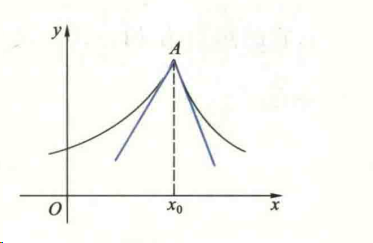
\includegraphics[width=\marginparwidth]{figures/screenshot001.png}
	\caption{$A$点两侧的切线}
	\label{fig:1.1}
\end{marginfigure}

\section{导数的几何意义}\label{sec:1.2}
因为高中接触切线比较多,此处不再多讲。

\subsection{几个切线的例子}\label{sec:1.2.1}

\subsubsection{左右导数存在却不相等}\label{sec:1.2.1.1}

\begin{marginfigure}[7em]
	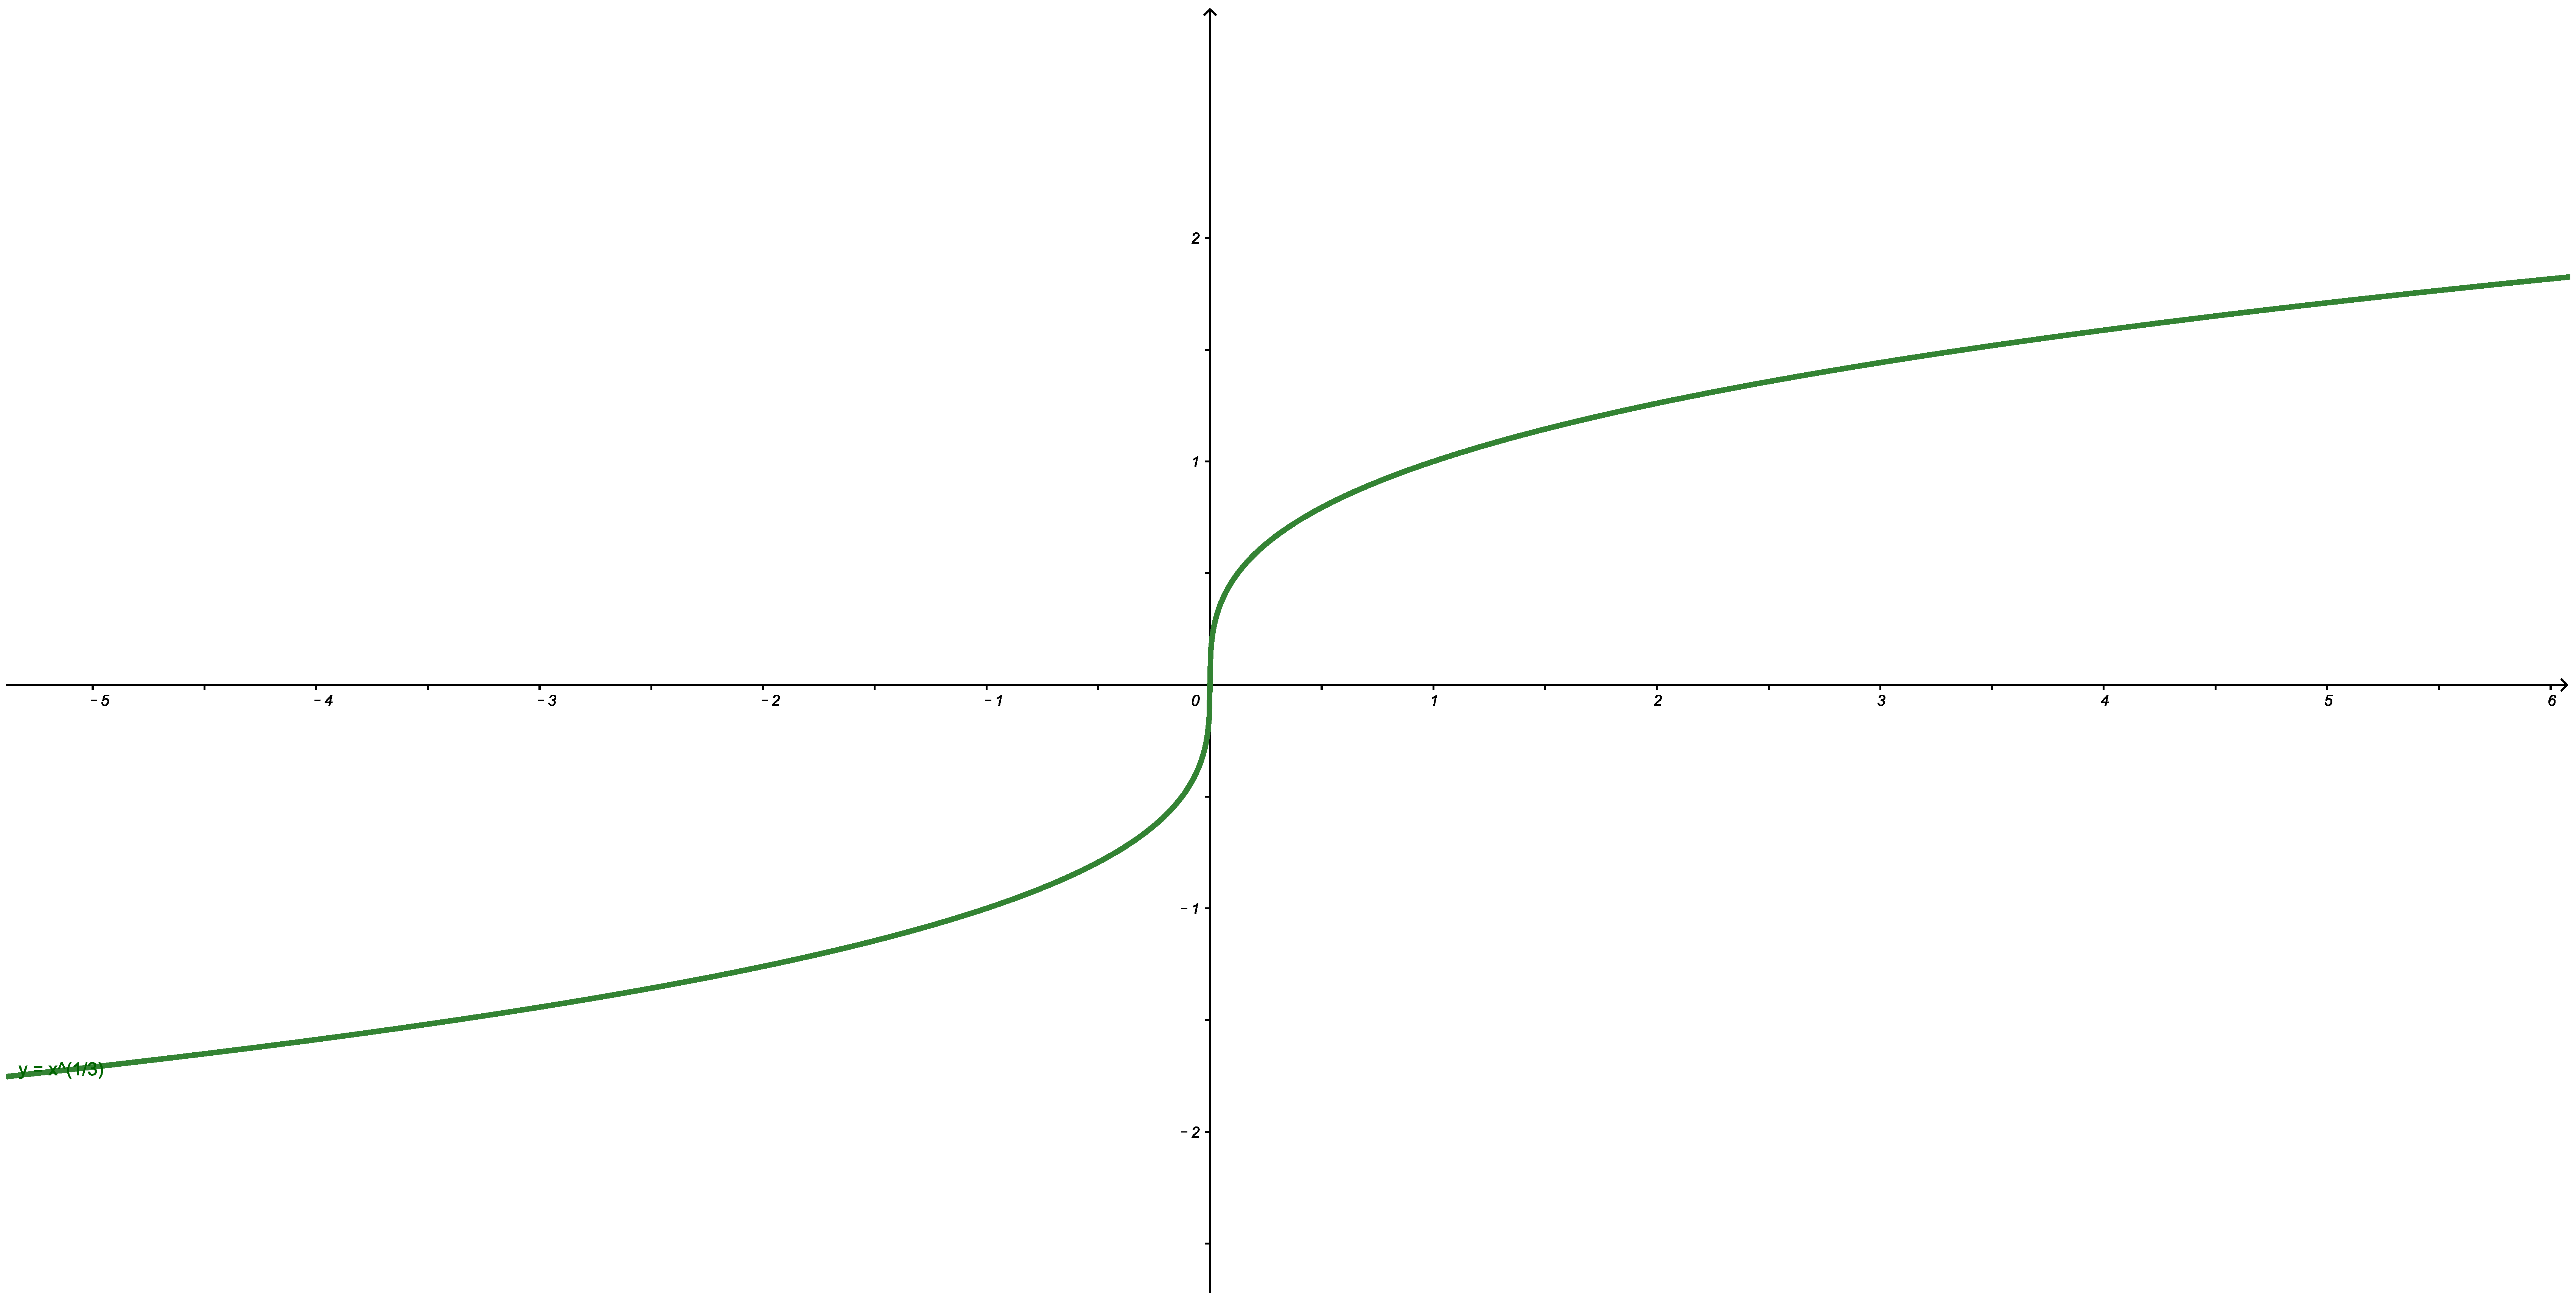
\includegraphics[width=\marginparwidth]{figures/2.eps}
	\caption{$O$点处的导数为正无穷}
	\label{fig:1.2}
\end{marginfigure}

高中学过,对于\textbf{可导函数},函数的导数在几何上表示曲线$y=f'(x)$在某点处的切线斜率。

对于\textbf{单侧导数存在的不可导函数},就把上面的表述更改为:\textbf{某侧导数表示某侧切线的斜率}。

图\ref{fig:1.1}所示的函数曲线,正好代表了某点在不同侧的切线,两条切线的斜率代表左右侧的导数值。如果左右导数存在且相等,那么两条切线二合一。

\subsubsection{导数的大小为正无穷}\label{sec:1.2.1.2}

如图\ref{fig:1.2}中$O$点处所示。

\subsubsection{不可导且曲线震荡}\label{sec:1.2.1.3}

如图\ref{fig:1.3}所示。

\begin{marginfigure}[7em]
	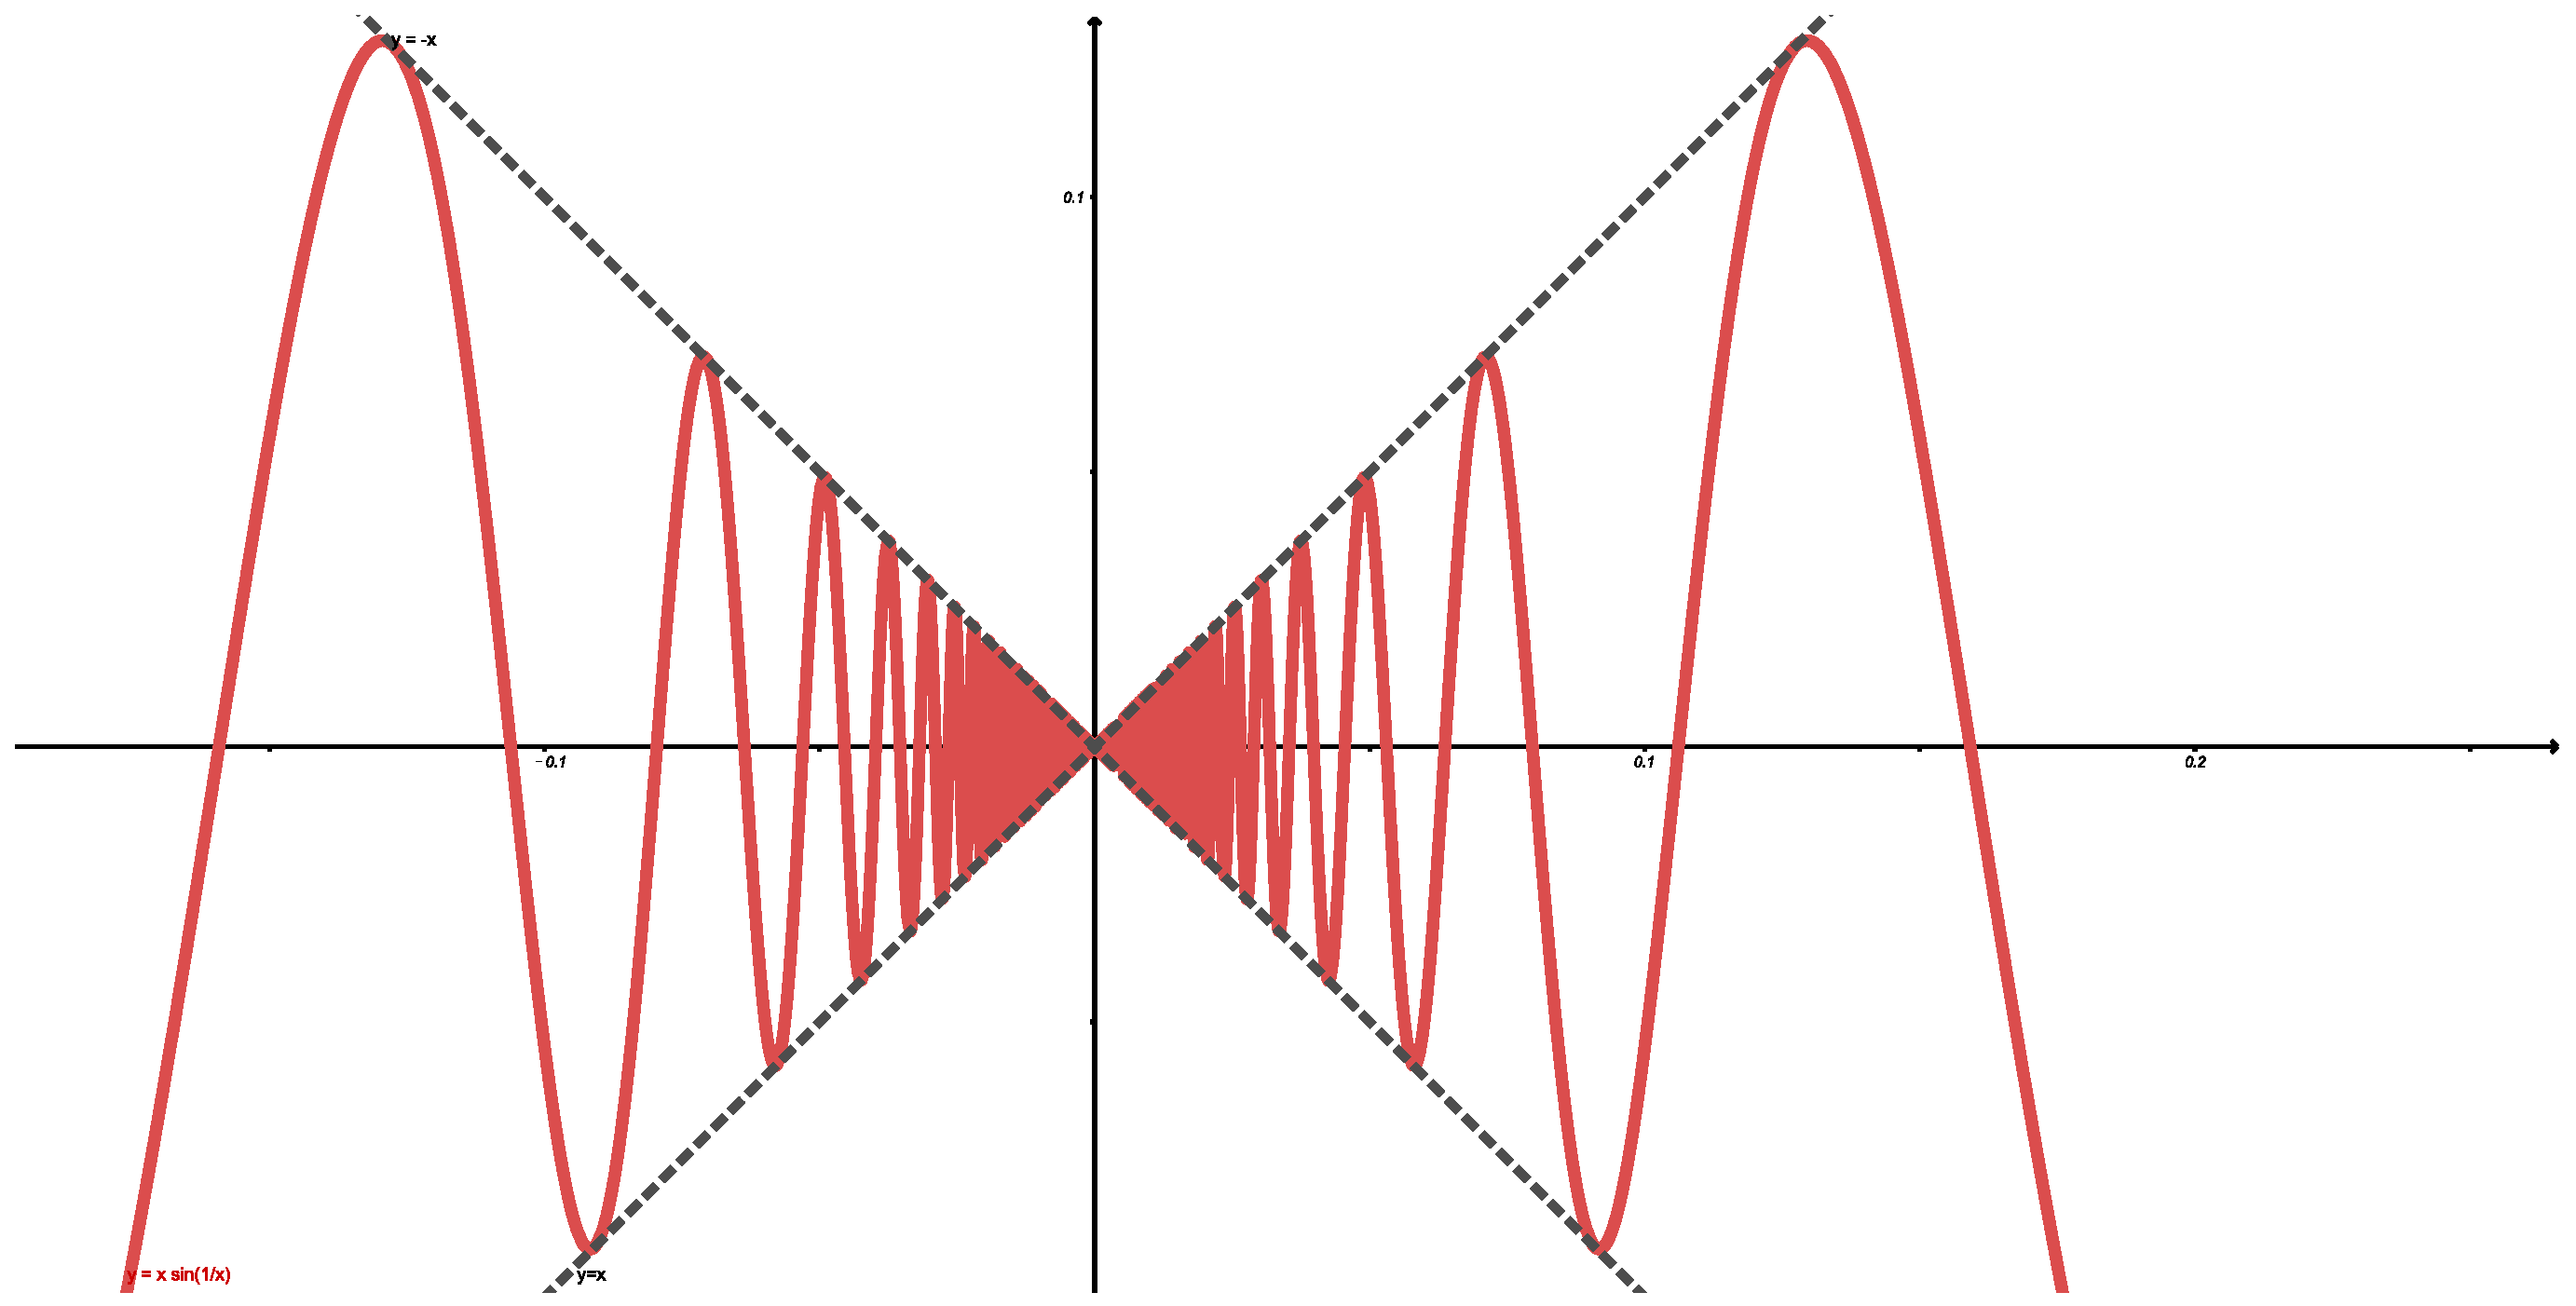
\includegraphics[width=\marginparwidth]{figures/3.eps}
	\caption{不可导且曲线震荡}
	\label{fig:1.3}
\end{marginfigure}

\section{模型、套路、题型}\label{sec:1.3}
\subsection{导数的存在}\label{sec:1.3.1}

\begin{problem}
	设$f(x)$在$x=0$处连续且$f(0)=0$,那么$f(x)$在$x=0$处可导的充分条件是\xparen
	\begin{xchoices}[showanswer = true]
		\item $\underset{\Delta x\rightarrow 0}{\lim}\frac{f(x)-f(-x)}{2x}$存在
		\item $\underset{\Delta x\rightarrow 0}{\lim}\frac{f\qty[\ln(1+x^2)]}{x^2}$存在
		\item $\underset{\Delta x\rightarrow 0}{\lim}\frac{f(x)}{\sqrt[3]{x}}$存在
		\item* $\underset{\Delta x\rightarrow 0}{\lim}xf\qty(\frac{1}{x})$
	\end{xchoices}
\vspace{0.5em}
\begin{solution}
	把握原则:“可导”$\Leftrightarrow$“左导数=右导数”。
	\begin{enumerate}[label=\Alph*.]
		\item 由$\underset{\Delta x\rightarrow 0}{\lim}\frac{f(x)}{x}$与$\underset{\Delta x\rightarrow 0}{\lim}\frac{f(-x)}{-x}$存在且相等$\Rightarrow\underset{\Delta x\rightarrow 0}{\lim}\frac{f(x)-f(-x)}{2x}$成立,但反之未必,此选项颠倒充分必要性。
		\item $\underset{\Delta x\rightarrow 0}{\lim} f(\ln(1+x^2))=\underset{\Delta x\rightarrow 0}{\lim}x^2\ge 0$因此不满足左右导数,只满足右导数。
		\item 显然不同阶。
		\item 如知识点叙述所说:$\underset{\Delta x\rightarrow \infty}{\lim}\frac{f(1/x)}{1/x}$存在,因此成立\mn{\textbf{总结反思:}在导数定义式中:
		\begin{enumerate}
			\item 微小变量需要可正可负;
			\item 分子分母的微小变量的表达式未必相同,但是极限值需要是1。
		\end{enumerate}}。
	\end{enumerate}
\end{solution}
\end{problem}
	
\subsection{导数与极限互化}\label{sec:1.3.2}

\begin{problem}
	设函数$y=f(x)$在点$x=0$处连续,且$\underset{\Delta x\rightarrow 0}{\lim}\frac{f(x)-2x}{1-\cos(x)}=1$,则在0处有\xparen
	
	\begin{xchoices}[showanswer = true]
		\item 不可导
		\item 可导且$f'(0)=0$
		\item 可导且$f'(0)=-2$
		\item* 可导且$\dd y\big|_{x=0} = 2\dd x$
	\end{xchoices}
	\vspace{0.5em}
	\begin{solution}
		\begin{enumerate}[label=(\Roman*)]
			\item 见到$1-\cos(x)$想到$\frac{1}{2}x^2$因此有$\underset{\Delta x\rightarrow 0}{\lim}\frac{2f(x)/x-4}{x}=1$,故有$\underset{\Delta x\rightarrow 0}{\lim}\frac{f(x)}{x}=2$,而显然$f(0)=0$,因此可导可微,且导数为2。
			\item $\underset{\Delta x\rightarrow 0}{\lim}f(x)=\frac{1}{2}x^2+2x$,故$\underset{\Delta x\rightarrow 0}{\lim}f'(x)=2+x$,所以可导,导数为2\mn{\textbf{总结反思:}由此题可以看出遇到这种形式的极限时,应该如何实现极限与导数的互化。解析中的思路(II)是编者自己第一次见到这个题目时候想到是不是能把表达式写出来,不一定对,如果不对请及时反映。}。
		\end{enumerate}
	\end{solution}
\end{problem}

\begin{problem}
	已知$f(x)$在$x=0$处连续,且$\underset{\Delta x\rightarrow 0}{\lim}[f(x)+e^x]^{\frac{1}{x}}=2$,则$f'(0)=$\xparen
	\begin{xchoices}[showanswer = true]
		\item 不存在
		\item $\ln(2)$
		\item $2$
		\item* $\ln(2)-1$
	\end{xchoices}
\vspace{0.9em}
    \begin{solution}
    	$\underset{\Delta x\rightarrow 0}{\lim}\frac{\ln[f(x)+e^x]}{x}=\ln2$\mn{取对数处理法是面对指数型极限的常用处理方式,由此题注意总结。},故$\underset{\Delta x\rightarrow 0}{\lim}\ln[f(x)+e^x]=0$,故$f(0)=0$,此时就形成了$\frac{f(x)}{x}$模型,而$\underset{\Delta x\rightarrow 0}{\lim}\frac{\ln[f(x)+e^x]}{x}=\underset{\Delta x\rightarrow 0}{\lim}\frac{f(x)+e^x-1}{x}=\ln2$,故得$f'(0)=-1+\ln(2)$。
    \end{solution}
\end{problem}

\begin{problem}
	对于$y=f(x)$,有$f(1)=0, f'(1)=1$,求$\underset{n\rightarrow \infty}{\lim}f\qty(\frac{n}{n+2})$的值。
	\begin{solution}
		显然属于极限导数互化,尝试构造$x=1$处的导数\mn{既然是已经给了某处的函数导数值,那就把它直接构造出来。}。
		$$
		\underset{n\rightarrow \infty}{\lim}n\cdot \frac{f\qty(1+\dfrac{-2}{n+2})-0}{\dfrac{-2}{n+2}\cdot\dfrac{n+2}{-2}}=\frac{-2n}{n+2}\cdot \underset{ n\rightarrow \infty}{\lim}f'(1)=-2
		$$
	\end{solution}
\end{problem}

\begin{problem}
	设$f(x)$在$x=a$处二阶可导,则极限$\underset{ x\rightarrow 0}{\lim}\frac{\dfrac{f(a+x)-f(a)}{x}-f'(a)}{x}=$\xparen
	\begin{xchoices}[showanswer = true]
		\item ${0}$
		\item ${f''(a)}$
		\item ${2f''(a)}$
		\item* ${\frac{f''(a)}{2}}$
	\end{xchoices}
\vspace{0.5em}
\begin{solution}
	第一眼看上去仿佛是:$\frac{f'(a)-f'(a)}{x}$,但是由于极限的:趋近而非完全相等的性质,需要进一步探究阶数与小量的关系。
	\begin{enumerate}[label=(\Roman*)]
		\item $\frac{f(a+x)-f(a)-xf'(a)}{x^2}$,进一步,由洛必达法则,有$\underset{ x\rightarrow 0}{\lim}\frac{f'(a+x)-f'(a)}{2x}=\frac{f''(a)}{2}$。
		\item $f(a+x)=f(a)+f'(a)x+\frac{f''(a)}{2!}x^2+o(x^2)$,则有$\underset{ x\rightarrow 0}{\lim}\frac{f(a+x)-f(a)-f'(a)x}{x^2}=\underset{ x\rightarrow 0}{\lim}\frac{\frac{f''(a)}{2}x^2+o(x^2)}{x^2}=\frac{f''(a)}{2}$\mn{认真体会思路(I)和(II)的区别与相通性:其实是洛必达与泰勒的相通性。}。
	\end{enumerate}
\end{solution}
\end{problem}

\subsection{可导性探源}\label{sec:1.3.3}

\begin{problem}
	已知函数$f(x) =\left|x-x^2\right|({\rm e}^x-1)+\sin|x-2|$的不可导点的个数为\xparen
	
	\begin{xchoices}[showanswer = true]
		\item 0
		\item 1
		\item* 2
		\item 3
	\end{xchoices}
	\vspace{0.5em}
	\begin{solution}
		不可导点一般模型有两种,此题为第一种,函数表达式明确。对于寻找不可导点,其实就是由外向内层层剥离函数。
		\begin{enumerate}[label=(\arabic*)]
			\item 简化函数表达式到最清晰的情况:$f(x)= |x||x-1|({\rm e}^x-1)+sin|x-2|$;
			\item 依次确定每个函数的特殊点\mn{对于绝对值形成的函数,可不可导的关键就是$\underset{\Delta x\rightarrow 0}{\lim}\frac{f(x+\Delta x)-f(x)}{\Delta x}$是否会因为绝对值的存在导致左右异号,此题中$|x|$函数因为有${\rm e}^x-1$的存在避免了这种情况。}:0、1、0、2;
			\item 对$x=0$,依据定义$\underset{ x\rightarrow 0}{\lim}\frac{f(x)-f(0)}{x}=\underset{\Delta x\rightarrow 0}{\lim}=\sin 2$,恒有左右导相等;
			\item 对$x=1$,依据定义$\underset{\Delta x\rightarrow 0}{\lim}\frac{f(1+\Delta x)-f(1)}{\Delta x}=\underset{\Delta x\rightarrow 0}{\lim}\pm|1+\Delta x|\qty({\rm e}^{|1+\Delta x|}-1)+\sin(-1+\Delta x)$,左右导不相等;
			\item 对$x=2$,同上,发现左右导数不相等。
		\end{enumerate}
	\end{solution}
\end{problem}

\begin{problem}
	$f(x)=\underset{ n\rightarrow \infty}{\lim}\sqrt[n]{1+|x|^n+{\rm e}^{nx}}$的不可导点个数为\xparen
	\begin{xchoices}[showanswer=true]
		\item 0
		\item 1
		\item* 2
		\item 3
	\end{xchoices}
\vspace{0.5em}
\begin{solution}
	此题的函数以极限形式出现,所以首先要给出不同区间上的函数表达式\mn{以极限形式出现的函数,要写出其具体形式,一般为分段函数。}。
	
	\begin{enumerate}[label=(\arabic*)]
		\item 对于$\underset{ n\rightarrow \infty}{\lim}{\rm e}^{nx}$,当$x\ge 0$时趋于正无穷,$x\le 0$时趋于0;
		\item 对于$\underset{ n\rightarrow \infty}{\lim}|x|^n$,当$x\in(-1,1)$时趋于0,反之趋于正无穷,但是是那种远小于${\rm e}^{nx}$的正无穷,证明即$\frac{|x|^n}{{\rm e}^{nx}}=\qty(\frac{x}{{\rm e}^x})^n=0$;
		\item 因此,由区间划分为
		$ f(x)=\left\{
		\begin{aligned}
			&-x,&x\le -1\\
			&1,&-1\leq x\geq 0\\
			&e^x,&x\ge 0
		\end{aligned}
		\right.
		$;
		\item 发现两个分界点:-1,0皆不可导。
	\end{enumerate}
\end{solution}
\end{problem}

\subsection{复杂求导方法与典型导数模型}\label{sec:1.3.4}

\begin{problem}
	已知$f(x)=\frac{(x-1)(x-2)...(x-n))}{(x+1)(x+2)...(x+n)}$,求$f'(1)$的值。
	\vspace{0.3em}
	\begin{solution}
		按部就班写出导数表达式,显然有$f(1)=0$,于是
		\begin{align*}
			f'(1)&=\underset{ x\rightarrow 1}{\lim}=\frac{\dfrac{(x-1)(x-2)...(x-n))}{(x+1)(x+2)...(x+n)}}{x-1}=\frac{(x-2)...(x-n))}{(x+1)(x+2)...(x+n)}\\
			&=\frac{(-1)^{n-1}(n-1)!}{(n+1)!}=\frac{(-1)^{n-1}}{n(n+1)}
		\end{align*}
	\end{solution}
\end{problem}

\begin{problem}
	已知$f(x)=\sqrt{\frac{(1+x)\sqrt{x}}{e^{x-1}}}$,求$f'(1)$的值。
	\begin{solution}
		显然采用对数求导法,按照如下格式。
		
		$\ln(g(x))=\frac{1}{2}[\ln(1+x)+\frac{1}{2}\ln(x)-(x-1)]$,$\frac{g'(x)}{g(x)}=\frac{1}{2}\qty(\frac{1}{x+1}+\frac{1}{2x}-1)$,$\frac{g'(1)}{g(1)}=0$,故$g'(1)=0$
	\end{solution}
\end{problem}

% \chapter{占位章}
\chapter{求导的基本法则}\label{ch:2}

本章讲述函数求导的基本法则,有一部分内容大家在高中就已经学习过,我们以复习为主,同时补充一些新细节,具体需要大家:

\begin{enumerate}
	\item \textbf{熟练掌握}函数四则运算的求导法则,复合函数的链导法则;
	\item \textbf{了解}反函数的求导法则;
	\item \textbf{熟记}基本初等函数的导数;
	\item \textbf{熟记}部分函数的高阶导数公式,\textbf{掌握}求高阶导数的方法;
	\item \textbf{掌握}隐函数的求导法,参数方程确定的函数的求导法则。
\end{enumerate}

\section{复习背景}\label{sec:2.1}

\subsection{导数的定义}\label{sec:2.1.1}

\begin{definition}
	设函数$f(x)$定义在$x_0$的某一邻域$U(x_0)$内,在此邻域内,当自变量在$x_0$处有改变量
	$\Delta{x}$时,相应的函数有改变量$\Delta{y}=f(x_0+\Delta{x})-f(x_0)$,若当$\Delta{x}\to{0}$时这两个改变量之比的极限
	
	\begin{equation}
		\lim_{\Delta{x}\to{0}}\frac{\Delta{y}}{\Delta{x}}=\lim_{\Delta{x}\to{0}}\frac{f(x_0+\Delta{x})-f(x_0)}{\Delta{x}}
		\label{eq:2.1}
	\end{equation}
	
	存在,则称函数$f$\textbf{在$x_0$处可导},并称该极限值为$f$\textbf{在$x_0$处的导数。}
\end{definition}

\subsection{反函数的定义}\label{sec:2.1.2}

\begin{definition}
	若$f$是A上的\textbf{严格单调增(减)}函数,则它必存在反函数$f^{-1}$,且反函数$f^{-1}$也是值域$f(A)$上的严格单调增(减)函数。
\end{definition}

\section{知识点初始——函数四则运算的求导法则}\label{sec:2.2}

\subsection{导数有理运算法则}\label{sec:2.2.1}

设函数$u,v$在某一个数域内可导,则有如下运算法则\mn{在计算商的导数时,切记分子上是先对原函数分子上的函数求导。}:

\begin{equation}
	\begin{split}
		&(u\pm{v})'(x)=u'(x)\pm{v'(x)}\\
		&(uv)'(x)=u'(x)v(x)+u(x)v'(x)\\
		&\qty(\frac{u}{v})'(x)=\frac{u'(x)v(x)-u(x)v'(x)}{v^2(x)},~(v(x)\neq{0})
	\end{split}\label{eq:2.2}
\end{equation}

\subsection{几个三角函数求导的例子}\label{sec:2.2.2}
我们将把以下几个高中不常见三角函数的求导过程作为导数有理运算的练习,请读者先自行计算,再参考过程。

\begin{example}
	计算$\tan{x}$的导数。
	\[(\tan{x})'=(\frac{\sin{x}}{\cos{x}})'=\frac{(\sin{x})'\cos{x}-\sin{x}(\cos{x})'}{\cos^2{x}}=\frac{\cos^2{x}+\sin^2{x}}{\cos^2{x}}=\sec^2{x}\]
\end{example}

\begin{example}
	计算$\sec{x}$的导数。
	\[(\sec{x})'=(\frac{1}{\cos{x}})'=-\frac{(\cos{x})'}{\cos^2{x}}=\frac{\sin{x}}{\cos^2{x}}=\sec{x}\tan{x}\]
\end{example}

按照上述的思路,我们可以得到

\begin{align*}
	&(\cot{x})'=-\csc^2{x}\\
	&(\csc{x})'=-\csc{x}\cot{x}
\end{align*}

请读者自行计算。

\section{知识点初始——复合函数的求导法则}\label{sec:2.3}

\subsection{求导的链式法则}\label{sec:2.3.1}
设函数$u=g(x)$在$x$处可导,函数$y=f(u)$在与$x$相对应的$u$处可导,则复合函数\mn{复合函数的链导法则要求内层和外层的两个函数均在对应点可导。}$y=f[g(x)]$在$x$处可导,并且:
\begin{equation}
	\frac{\mathrm{d}y}{\mathrm{d}x}=f'(u)\cdot g'(x)\label{eq:2.3}
\end{equation}
或
\begin{equation}
	\frac{\mathrm{d}y}{\mathrm{d}x}=\frac{\mathrm{d}y}{\mathrm{d}u}\cdot\frac{\mathrm{d}u}{\mathrm{d}x}\label{eq:2.4}
\end{equation}

\begin{remark}
	链导法则的名称非常形象,当函数有多层复合时,首先弄清复合关系,再\textbf{由外向内}一层一层逐个求导,这是链导法则的推广。
\end{remark}

\subsection{利用链式法则计算双曲函数的导数}\label{sec:2.3.2}

\begin{example}
	求双曲正弦函数$y = {\rm sh}(x) = \frac{{\rm e}^x-{\rm e}^{-x}}{2}$的导数。
	\[({\rm sh}(x))'=\frac{1}{2}[({\rm e}^x)'-({\rm e}^{-x})']\]
	又$u={\rm e}^{-x}$可以看成是$u={\rm e}^t$与$t=-x$的复合函数,所以
	\[\frac{\mathrm{d}u}{\mathrm{d}x}=({\rm e}^{-x})'=\frac{\mathrm{d}u}{\mathrm{d}t}\cdot\frac{\mathrm{d}t}{\mathrm{d}x}={\rm e}^t\cdot{(-1)}=-{\rm e}^{-x}\]
	因此
	\[({\rm sh}(x))'=\frac{1}{2}({\rm e}^x+{\rm e}^{-x})={\rm ch}(x)\]
	同理可以求得
	\[({\rm ch}(x))'={\rm sh}(x)\]
	\[({\rm th}(x))'=\frac{1}{{\rm ch}^2(x)}\]
\end{example}

\begin{remark}
	(1)双曲函数是同学们上大学来第一次接触,需要同学们重点记忆。一方面在期中考试当中会有非常小的概率考察到;另一方面,在积分的第二类换元法中也有机会用到双曲函数。(2)熟练掌握链式求导法则以后,可以不再写出中间变量,提高做题的速度。
\end{remark}

\section{知识点初始——反函数的求导法则}\label{sec:2.4}

\subsection{反函数的求导法则}\label{sec:2.4.1}

设区间$I$上的严格单调连续\mn{严格单调连续的条件可以省略,在应用反函数求导法则时,只需要验证$f'(y)\neq{0}(y\in{I})$即可。}函数$x=f(y)$在点$y$处可导,且$f'(y)\neq{0}$,则它的反函数$y=f^{-1}(x)$在对应点$x$处可导,并且
\begin{equation}
	(f^{-1})'(x)=\frac{1}{f'(y)}\label{eq:2.5}
\end{equation}
或
\begin{equation}
	\frac{\mathrm{d}y}{\mathrm{d}x}=\frac{1}{\mathrm{d}x/\mathrm{d}y}\label{eq:2.6}
\end{equation}

可以简单理解为:\textbf{若两个函数互为反函数,则它们的导数互为倒数。}

\subsection{利用反函数的求导法则求反三角函数的导数}\label{sec:2.4.2}
\begin{example}
	求反正弦函数$y=\arcsin{x},~x\in{(-1,1)}$的导数。
	
	由于其为正弦函数$x=\sin{y},~y\in{\qty(-\frac{\pi}{2},\frac{\pi}{2})}$的反函数,并且当$y\in{\qty(-\frac{\pi}{2},\frac{\pi}{2})}$时,$(\sin{y})'=\cos{y}\neq{0}$,所以定理的所有条件都满足,则在区间$(-1,1)$有
	
	\[(\arcsin{x})'=\frac{1}{(\sin{y})'}=\frac{1}{\cos{y}}=\frac{1}{\sqrt{1-\sin^2{y}}}=\frac{1}{\sqrt{1-x^2}},~ x\in{(-1,1)}\]
	
	同理可得
	
	\[(\arccos{x})'=-\frac{1}{\sqrt{1-x^2}}\]
	\[(\arctan{x})'=\frac{1}{1+x^2}\]
\end{example}

\begin{remark}
	反三角函数大多数同学在高中接触不多,但在以后的学习中会经常用到,牢记反三角函数的导数对后期大家做积分题目的时候会有很大的帮助,反三角函数导数可以和三角函数类比记忆,其正负号的关系刚好与三角函数的求导相反。
\end{remark}

\section{知识点初始——初等函数的求导问题}\label{sec:2.5}

初等函数是由基本初等函数经过有限次有理运算和复合运算构成的,可以利用导数的有理运算法则以及链式法则求得初等函数的导数。并且\textbf{可导初等函数的导数仍为初等函数}。在\textcolor{lbexacolor}{\ref{app:1}}\mn{点击红字即可跳转至附录A。}中给出基本初等函数的导数公式表。

\section{知识点初始——高阶导数}\label{sec:2.6}

\subsection{高阶导数的定义}\label{sec:2.6.1}

\begin{definition}
	若$f$的$n-1$阶导函数$f^{(n-1)}:I\to{\mathbb{R}}$在$x\in{I}$可导,则称$f$在$x$处\textbf{$n$阶可导},$f^{(n-1)}$在$x$处的导数称为$f$在$x$处的\textbf{$n$阶导数},记作$f^{(n)}(x)=(f^{(n-1)})'(x)$.若$f$在$I$上处处$n$阶可导,则称$f$\textbf{在$I$上$n$阶可导},$f^{(n)}$称为$f$在$I$上的\textbf{$n$阶导函数},简称\textbf{$n$阶导数}。
\end{definition}

\subsection{连续可导的定义}\label{sec:2.6.2}

\begin{definition}
	若$f^{(n)}$在$I$上连续,则称$f$在$I$上\textbf{$n$阶连续可导},或称$f$为$I$上的\textbf{$C^{(n)}$类函数},记作$f\in{C^{(n)}(I)}$。
\end{definition}

\begin{remark}
	$f(x)n$阶可导和$f(x)\in{C^{(n)}}$的区别:
	
	(1)$n$阶可导表明$f(x)$有$n$阶导数,但$f^{(n)}(x)$不一定连续;
	
	(2)$f(x)\in{C^{(n)}}$表明在$n$阶可导的基础上,$f^{(n)}(x)$连续。
	
	一般证明题中给出条件为$f(x)\in{C^{(n)}}$,但有时会给$f(x)$为$n$阶可导,希望同学们分辨清楚。
\end{remark}

\section{知识点初始——隐函数求导法}\label{sec:2.7}

\subsection{隐函数的求导法}\label{sec:2.7.1}

设由方程$F(x,f(x))\equiv 0$确定了一个隐函数$y=f(x)$.则在求导的时候很容易看出$F$是一个复合函数,利用复合函数的链导法则,方程两边同时对$x$求导,可以求得隐函数的导数\mn{(1)隐函数导数的几何意义同样是曲线的切线,因此在求曲线的切线方程中有重要意义。\\(2)准确来说,隐函数导数是建立在隐函数存在且可导的基础之上的,同时隐函数可以是一个局部概念。例子中圆的方程整体上是无法确定一个隐函数的,但是在第一象限是可以确定的;同时各个象限隐函数的导数形式是一致的。在习题当中,同学们不用考虑隐函数的存在性和可导性,只需要掌握求导方法就可以。}。

\subsection{隐函数求导的注意点}\label{sec:2.7.2}

\begin{example}
	求由方程$x^2+y^2=1$所确定的隐函数的导数。
	
	利用隐函数的求导法,对方程两边求导得:
	\[2x+2yy'=0\]
	移项得
	\[y'=-\frac{x}{y}\]
\end{example}

\section{由参数方程确定的函数的求导法则}\label{sec:2.8}

\subsection{求一阶导数}\label{sec:2.8.1}

若函数$x=x(t)$与$y=y(t)$在某个区间上可导,且$x'(t)\neq 0$,则有:

\begin{equation}
	\frac{\mathrm{d}y}{\mathrm{d}x}=\frac{y'(t)}{x'(t)}\label{eq:2.7}
\end{equation}

\begin{remark}
	一阶导数的求导非常容易记忆,简记为上下同时求导。
\end{remark}

\subsection{求二阶导数}\label{sec:2.8.2}

二阶导数公式有两种形式,对应两种不同的使用情况。

\subsubsection{求导数的数学表达式}

\begin{equation}
	\frac{\mathrm{d}^2y}{\mathrm{d}x^2}=\frac{\mathrm{d}}{\mathrm{d}t}(\frac{y'(t)}{x'(t)})\cdot \frac{1}{x'(t)}\label{eq:2.8}
\end{equation}

\begin{remark}
	该公式可以简记为,一阶导数对参数求导,再除以自变量的一阶导数。在题目要求求出表达式时,建议使用该形式。
\end{remark}

\subsubsection{求某点二阶导数的值}

\begin{equation}
	\frac{\mathrm{d}^2y}{\mathrm{d}x^2}=\frac{x'(t)y''(t)-x''(t)y'(t)}{(x'(t))^3}\label{eq:2.9}
\end{equation}

\begin{remark}
	该形式实际上是上一种的展开,利用商的求导法则可以快速记忆。在求具体值时,利用该形式可以分块计算,避免求导过程中的错误和冗长的算式带来的计算错误。
\end{remark}

\subsection{含隐函数形式的参数求导}\label{sec:2.8.3}
当函数的参数形式变为$F(x,t)=0, G(y,t)=0$时,需要同时利用隐函数求导和参数求导,具体方法为:

\begin{enumerate}
	\item 单独对每个方程使用隐函数求导,解出$x'(t)$,$y'(t)$;
	\item 利用参数方程求导的公式,结合对参数的一阶导数,来解出答案。
\end{enumerate}

\section{求高阶导数的方法}\label{sec:2.9}

\subsection{常见函数的高阶导数公式}\label{sec:2.9.1}

\begin{equation}
	\begin{split}
		&({\rm e}^x)^{(n)} = {\rm e}^x\\
		&(\sin{x})^{(n)} = \sin{\qty(x+n\cdot \frac{\pi}{2})}\\
		&(\cos{x})^{(n)}=\cos{\qty(x+n\cdot \frac{\pi}{2})}\\
		&(x^{\alpha})^{(n)}=\alpha (\alpha -1)\cdots (\alpha -n+1)x^{\alpha -n}\quad (\alpha\in{\mathbb{R}},x>0)\\
		&[\ln{(1+x)}]^{(n)}=(-1)^{(n-1)}\frac{(n-1)!}{(1+x)^n}\quad (x>-1)
	\end{split}\label{eq:2.10}
\end{equation}

\begin{remark}
	牢记这些高阶导数公式对理解和记忆下一节的Taylor公式有很大的帮助,同时也是利用Leibniz公式的基础。
\end{remark}

\subsection{利用归纳法求高阶导数}

对于部分函数而言,可以先求出几阶导数,观察导数的特点和规律,猜出其高阶导数的形式,再利用数学归纳法证明\mn{填空题和选择题可以忽略证明过程,但最好检验一下找到的规律。}。

\subsection{利用Leibniz公式求高阶导数}\label{sec:2.9.2}

\subsubsection{Leibniz公式}

设函数$u,v$都是$n$阶可导,则$\alpha u+\beta v$与$uv$也是$n$阶可导的,并且有:

\begin{enumerate}
	\item 线性性质\quad $(\alpha u+\beta v)^{(n)}=\alpha u^{(n)}+\beta v^{(n)},\quad \alpha,\beta\in{\mathbb{R}}$;
	\item Leibniz公式\mn{可以类比二项式定理来记忆该公式。}
	\begin{equation}
		(uv)^{(n)}=\sum^n_{k=0}C^k_nu^{(n-k)}v^{(k)}\label{eq:2.11}
	\end{equation}
\end{enumerate}

\subsubsection{使用Leibniz公式的情况和两个函数的选择}

\begin{example}
	已知$f(x)=x^3\sin{x}$,求$f^{(n)}(x)$。
	
	取$u=\sin{x},v=x^3$,根据公式\mn{在出现多项式函数和已知高阶导数的函数乘积时,可以考虑使用Leibniz公式。}可得
	\begin{align*}
		f^{(n)}(x)=&x^3(\sin{x})^{(n)}+n\cdot 3x^2(\sin{x})^{(n-1)}+\frac{n(n-1)}{2!}\cdot 6x(\sin{x})^{(n-2)}+\frac{n(n-1)(n-2)}{3!}\\
		&\cdot 6(\sin{x})^{(n-3)}
	\end{align*}
\end{example}

由于多项式求导的特殊性,一般将多项式函数设为$u$函数,以便在几次展开后以后的项均为0,简化计算。

\subsection{利用Taylor公式求高阶导数}\label{sec:2.9.4}

Taylor公式一般处理求$f^{(n)}(0)$的情况。当函数为一个可以用麦克劳林公式展开的因式和多项式相乘的形式时,考虑使用该方法,具体步骤为:

\begin{enumerate}
	\item 将可展开的因式进行麦克劳林展开,找到对应阶数的项;
	\item 将整个函数进行麦克劳林展开,写成麦克劳林公式的形式;
	\item 利用Taylor公式的系数为$\frac{f^{(n)}(0)}{n!}$的特点,求出答案。
\end{enumerate}

\begin{example}
	已知$f(x)=x^2\ln{(1+2x)}$,求$f^{(2014)}(0)$。
	
	根据麦克劳林公式:
	\begin{align*}
		&\ln{(1+x)}=x-\frac{x^2}{2}+\cdots +\frac{x^{2013}}{2013}-\frac{x^{2014}}{2014}+o(x^{2014}) \\
		&\ln{(1+2x)}=2x-\frac{2^2 x^2}{2}+\cdots +\frac{2^{2013} x^{2013}}{2013}-\frac{2^{2014} x^{2014}}{2014}+o(x^{2014}) \\
		&f(x)=2x^3-\frac{2^2}{2}x^4+\cdots +\frac{2^{2013}}{2013}x^{2015}-\frac{2^{2014}}{2014}x^{2016}+o(x^{2016})
	\end{align*}
	
	根据Taylor公式:
	\[f(x)=f(0)+f'(0)x+\frac{f''(0)}{2!}x^2+\cdots+\frac{f^{(2014)}(0)}{2014!}x^{2014}+R_{2014}(x)\]
	由待定系数法\mn{该方法的本质是待定系数法,在对应系数时,注意不是两个公式的阶数对应,而是两个公式的次数对应。同时要确保将次数相同的项合并在一起。},次数相同的项系数相同,得
	\begin{align*}
		&-\frac{2^{2012}}{2012}=\frac{f^{(2014)}(0)}{2014!} \\
		&f^{(2014)}(0)=-\frac{2^{2012}}{2012}\cdot 2014!
	\end{align*}
\end{example}

\section{幂指函数的求导方法}\label{sec:2.10}
简单来说,我们将底数和指数上都存在自变量的函数称为幂指函数。

\subsection{指数求导法}\label{sec:2.10.1}
设$f(x)=u(x)^{v(x)}$,取指数得$f(x)={\rm e}^{v(x)\ln{u(x)}}$,再利用导数的四则运算以及链导法则即可完成。

\subsection{对数求导法}\label{sec:2.10.2}

设$y=u(x)^{v(x)}$,取对数得$\ln{y}=v(x)\ln{u(x)}$,移项后可以得到一个方程,$y$变为这个方程所确定的隐函数,利用隐函数的求导法则即可完成。

\begin{remark}
	对数求导法同所有隐函数求导一样,在不可导点和函数值为0的点的说明上会存在一些瑕疵,感兴趣的同学可以自行研究。以后做题当中不用讨论,直接应用即可。
\end{remark}

\section{习题}\label{2.11}

\subsection{基础题}\label{2.11.1}

\begin{problem}
	设函数$y=y(x)$由方程$x^2-y+1={\rm e}^y$确定,求$\frac{\mathrm{d}^2y}{\mathrm{d}x^2}$。
	\begin{solution}
		方程两边关于$x$求导得:
		\begin{equation}
			2x-\frac{\mathrm{d}y}{\mathrm{d}x}={\rm e}^x\frac{\mathrm{d}y}{\mathrm{d}x}\label{eq:2.12}
		\end{equation}
	
		即
		
		\[y'=\frac{2x}{1+{\rm e}^y}\]
		
		对式(\ref{eq:2.12})两边关于$x$求导,得
		
		\[{\rm e}^y\qty(\frac{\mathrm{d}y}{\mathrm{d}x})^2+(1+{\rm e}^y)\frac{\mathrm{d}^2y}{\mathrm{d}x^2}=2\]
		
		将一阶导数代入,移项化简得:
		
		\[\frac{\mathrm{d}^2y}{\mathrm{d}x^2}=\frac{2-{\rm e}^y\qty(\dfrac{\mathrm{d}y}{\mathrm{d}x})^2}{1+{\rm e}^y}=\frac{2(1+{\rm e}^y)^2-4x^2{\rm e}^y}{(1+{\rm e}^y)^3}\]
	\end{solution}
\end{problem}

\begin{problem}
	已知摆线的参数方程为
	\begin{equation*}
		\left\{
		\begin{aligned}
			&x=a(t-\sin{t})\\
			&y=a(1-\cos{t})
		\end{aligned}
		\right.
	\end{equation*}
    \begin{enumerate}[label=(\arabic*)]
    	\item 求摆线上任一点的切线和法线斜率;
    	\item 求由该参数方程所确定的函数的二阶导数$\frac{\mathrm{d}^2y}{\mathrm{d}x^2}$。
    \end{enumerate}
    
    \begin{solution}
    	\begin{enumerate}[label=(\arabic*)]
    		\item 通过参数方程的求导法则得:
    		\begin{align*}
    			&k_1=\frac{\mathrm{d}y}{\mathrm{d}x}=\frac{a\sin{t}}{a(1-\cos{t})}=\frac{\sin{t}}{1-\cos{t}}\\
    			&k_2=-\frac{1}{k_1}=\frac{1-\cos{t}}{\sin{t}}
    		\end{align*}
    		\item 由(1)中已经求得的一阶导数,利用参数方程求导的第一种形式
    		\begin{align*}
    			\frac{\mathrm{d}^2y}{\mathrm{d}x^2}&=\frac{\mathrm{d}}{\mathrm{d}x}\qty(\frac{\sin{t}}{1-\cos{t}})\\
    			&=\frac{\mathrm{d}}{\mathrm{d}t}\qty(\frac{\sin{t}}{1-\cos{t}})\cdot\frac{\mathrm{d}t}{\mathrm{d}x}\\
    			&=\frac{\cos{t}(1-\cos{t})-\sin^2{t}}{(1-\cos{t})^2}\cdot\frac{1}{a(1-\cos{t})}\\
    			&=-\frac{1}{a(1-\cos{t})^2}
    		\end{align*}
    	\end{enumerate}
    \end{solution}
\end{problem}

\begin{problem}
	设$y=\frac{1}{x^2+5x+6}$,求$y^{(100)}$。
	
	\begin{solution}
		\[y=\frac{1}{x^2+5x+6}=\frac{1}{(x+2)(x+3)}=\frac{1}{x+2}-\frac{1}{x+3}\]
		
		根据高阶导数公式
		\[(\frac{1}{ax+b})^{(n)}=\frac{(-1)^nn!a^n}{(ax+b)^{n+1}}\]
		
		代入,得
		\[y^{(100)}=\frac{(-1)^{100}100!}{(x+2)^{101}}-\frac{(-1)^{100}100!}{(x+3)^{101}}\]
	\end{solution}
\end{problem}

\begin{problem}
	设$f(x)=x^2\sin{x}$,对于$n\geq 1$时,求$f^{(2n)}(0)$。
	
	\begin{solution}
		令$u=x^2,v=\sin{x}$,由Leibniz公式得
		
		\[(uv)^{2n}=\sum^{2n}_{k=0}C^k_{2n}u^{(2n-k)}v^{(k)}\]
		
		由于$u(0)=0,u'(0)=0,u''(0)=2$,当$k\geq 3$时,$u^{(k)}(0)=0$,所以
		
		\[(x^2\sin{x})^{(2n)}=C^{2n-2}_{2n}2(\sin{x})^{(2n-2)}\]
		
		由于
		\[(\sin{x})^{(2n-2)}\big|_{x=0}=\sin{(x+\frac{(2n-2)\pi}{2})}\Big|_{x=0}=0\]
		
		所以原式$=0$。
	\end{solution}
\end{problem}

\begin{problem}
	求函数$y=x^x$的导数
	
	\begin{solution}
		由对数求导法,方程两侧同时取对数,得
		\[\ln{y}=x\ln{x}\]
		
		利用隐函数求导,两端同时对$x$求导,得
		\[\frac{y'}{y}=1+\ln{x}\]
		
		化简,得
		\[y'=x^x(1+\ln{x})\]
	\end{solution}
\end{problem}

\subsection{提高题及思考题}

\begin{problem}
	设$y=f(x)$由以下两个方程确定:
	\begin{equation*}
		\left\{ 
		\begin{aligned}
			&x=t^2+2t\\
			&t^2-y+a\sin{y}=1
		\end{aligned}
		\right.
	\end{equation*}
	若$y(0)=b$,求$\frac{\mathrm{d}^2y}{\mathrm{d}x^2}\Big|_{t=0}$。
	
	\begin{solution}
		这是一个参数方程求导和隐函数求导的综合题,方程组两边同时对$t$求导,得
		\begin{equation*}
			\left\{ 
			\begin{aligned}
				&x'(t)=2t+2\\
				&2t-y'+a\cos{y}\cdot y'=0
			\end{aligned}
			\right.
		\end{equation*}
	
		化简,得
		\begin{equation*}
			\left\{ 
			\begin{aligned}
				&x'(t)=2(t+1)\\
				&y'(t)=\frac{2t}{1-a\cos{y}}
			\end{aligned}
			\right.
		\end{equation*}
	
		求得一阶导数
		\[\frac{\mathrm{d}y}{\mathrm{d}x}=\frac{y'(t)}{x'(t)}=\frac{t}{(1+t)(1-a\cos{y})}\text{并且}\frac{\mathrm{d}y}{\mathrm{d}x}\Big|_{t=0}=0\]
		
		进一步,求得二阶导数
		\[\frac{\mathrm{d}^2y}{\mathrm{d}x^2}=\frac{(\mathrm{d}y/\mathrm{d}x)'_t}{x'(t)}=\frac{\dfrac{(1-a\cos{y}-at(t+1)\sin{y}\cdot y'}{(t+1)^2(1-a\cos{y})^2}}{2(t+1)}\]
		
		注意到$y\big|_{t=0}=b,y'\big|_{t=0}=0$,得
		
		\[\frac{\mathrm{d}^2y}{\mathrm{d}x^2}=\frac{1}{2(1-a\cos{b})}\]
	\end{solution}
\end{problem}

\begin{problem}
	设$y={\rm e}^{ax}\sin{bx}$($a,b$为非零常数),求$y^{(n)}$。
	
	\begin{solution}
		利用欧拉公式\mn{${\rm e}^{xi}=\cos{x}+i\sin{x}$},将三角函数化为指数函数,再计算导数。
		
		令$u={\rm e}^{ax}\cos{bx},v={\rm e}^{ax}\sin{bx}$,则
		
		\begin{align*}
			u^{(n)}+iv^{(n)}&=(u+iv)^{(n)}=[{\rm e}^{ax}(\cos{bx}+i\sin{bx})]^{(n)}\\
			&=[{\rm e}^{(a+bi)x}]^{(n)}=(a+bi)^n {\rm e}^{(a+bi)x}\\
			&=(a^2+b^2)^{\frac{n}{2}}{\rm e}^{ax}[\cos{(bx+n\varphi)}+i\sin{(bx+n\varphi)}]
		\end{align*}
		
		由此得
		\[({\rm e}^{ax}\sin{bx})^{(n)}=(a^2+b^2)^{\frac{n}{2}}{\rm e}^{ax}\sin{(bx+n\varphi)},~\varphi=\arctan{\frac{b}{a}}\]
	\end{solution}
\end{problem}

\begin{problem}[思考题]
	设$y=\arctan{x}$,求$y^{(n)}(0)$。
	
	\begin{solution}
		逐次求导难以找到高阶导数得规律,考虑利用Leibniz公式,因为
		\[y'=\frac{1}{1+x^2}\]
		
		即
		\[(1+x^2)y'=1\]
		
		对两端求$n$阶导数,利用Leibniz公式
		\[\sum^n_{k=0}C^k_n(1+x^2)^{(k)}(y')^{(n-k)}=(1+x^2)\cdot y^{(n+1)}+2nxy^{(n)}+n(n-1)y^{(n-1)}=0\]
		
		令$x=0$,得
		\[y^{(n+1)}(0)=-n(n-1)y^{(n-1)}(0)\]
		
		在该递推公式基础上再加上$y'(0)=1,y''(0)=0$可得$n$为偶数时,$y^{(n)}(0)=0$;$n$为奇数时,$y^{(n)}(0)=(-1)^{\frac{n-1}{2}}(n-1)!$。
	\end{solution}
\end{problem}

% \chapter{占位章}
\chapter{微分}\label{ch:3}

微分顾名思义就是微积分中的“微分”部分。微分的概念立足于导数,搭桥到积分,是从求导到积分的桥梁。

\textbf{本节的要义不在于习题,而在于对于知识点的理解},只有切实理解了微分的具体概念,才能打好积分的基础,现在对本章的重点说明如下:

\begin{enumerate}
	\item 理解从导数到微分的来源的知识点。
	\item 从几何意义上理解微分。
	\item 熟练进行微分计算于高阶微分的求解。
\end{enumerate}

\section{背景回顾——从导数到积分}\label{sec:3.1}

\subsection{从公式的推导意义上}\label{sec:3.1.1}

由\textbf{前面所学的}导数的概念,有

\begin{equation}
	\frac{\Delta y}{\Delta x}=f'(x_0)+\frac{o(\Delta x)}{\Delta x}=f'(x_0)\label{eq:3.1}
\end{equation}

因此得到

\begin{equation}
	\Delta y=f'(x_0)\Delta x+o(\Delta x)\label{eq:3.2}
\end{equation}

\subsection{从数学背景上}\label{sec:3.1.2}

取函数$y=x^2$,易知$\Delta y=(x+\Delta x)^2-x^2=2x\Delta x+(\Delta x)^2$,由\textbf{前面所学的}阶数的比较,我们发现$(\Delta x)^2$比$2x\Delta x$阶数更高,当$\Delta x\rightarrow 0$时,相比$2x\Delta x$,$(\Delta x)^2$可以忽略,因此$\Delta y$的值主要取决于第一部分,我们称之为线性主部(关于$\Delta x$的一次项),\textbf{即在微小局部,用线性函数近似代替非线性函数}。

\begin{marginfigure}[1em]
	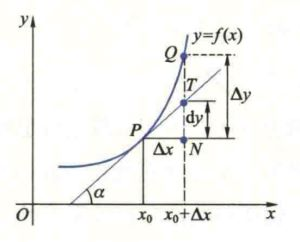
\includegraphics[width=\marginparwidth]{figures/导数的几何意义}
	\caption{导数的几何意义}
	\label{fig:3.1}
\end{marginfigure}

\subsection{从几何意义上}

由\textbf{前面所学的}导数的几何意义,如图\ref{fig:3.1}所示:

我们知道有:当$PN$趋近无穷小的时候,$TN\approx QN$,因此又由$\tan\alpha=f'(x_0)$,故有$f(x)\approx f(x_0)+f'(x_0)(x-x_0)$,\textbf{即在微小局部,用切线段似代替曲线段}。



\section{微分的概念}

\begin{definition}
	设有函数$f:U(x_0)\rightarrow \mathbb{R}$,若存在$\alpha \Delta x$,使$$f(x+\Delta x)-f(x_0)=\alpha\Delta x+o(\Delta x)$$
	\textbf{则称$f$在$x_0$处可微,$\alpha \Delta x$是其微分,记为$\dd f(x_0)=\alpha\Delta x$}
\end{definition}

\subsubsection{微分与导数的关系}

由$\dv{y}{x} = f'(x)$,导数等于函数的微分与之便利的微分之商,因此导数也称为微商。

由式\ref{eq:3.1}的推导,得到:\textbf{可微$\Leftrightarrow$可导}。两个概念互通,所以不区分。

\section{微分的运算、复合与高阶微分}\label{sec:3.3}

\subsection{导数的运算、复合与高阶微分}\label{sec:3.3.1}

请读者自行参考第 \ref{ch:2} 章的内容。

\subsection{微分的运算、复合与高阶微分}\label{sec:3.3.2}
由导数与微分的关系,可以得到
\begin{align*}
	&\dd (u\pm v)=du\pm dv\\
	&\dd(uv)=vdu+udv\\
	&\dd\qty(\frac{u}{v}) = \frac{v\dd u-u\dd v}{v^2}
\end{align*}

设有可微函数$y=f(u)$,而$u$又是另一个变量$x$的可微函数$u=g(x)$,那么复合函数$y=f(g(x))$的微分为

\begin{equation}
	\dd y = f'(u)g'(x)\dd x \label{eq:3.3}
\end{equation}

而我们知道$g'(x)\dd x = \dd u$,故上式可以写为
\begin{equation}
	\dd y = f'(u)\dd u \label{eq:3.4}
\end{equation}

这一性质称为\textbf{微分形式不变性}。

高阶微分,顾名思义就是对一阶微分再求一阶微分,即
\begin{equation*}
	\dd (\dd y) = \dd(f'(x)\dd x) = f''(x)(\dd x)^2
\end{equation*}
也即
\begin{equation}
	\dd^2 f = \dd^2 y = f''(x)\dd x^2\label{eq:3.5}
\end{equation}
对$n$阶微分
\begin{equation}
	\dd^n y = \dd^n f = f^{(n)}\dd x^n\label{eq:3.6}
\end{equation}

\section{微分在近似计算中的应用}\label{sec:3.4}
我们前面说到,微分是在微小局部中用线性主部代替主体的一种思想,那么当我们遇到某些难于计算却存在\textbf{与常见数值只差一个微小局部的计算题}时,我们就可以采用微分进行近似计算,即
\begin{equation}
	f(x+\Delta x)\approx f(x_0)+\alpha\Delta x\label{eq:3.7}
\end{equation}

常用的包括以下近似:
\begin{align*}
	&e^x\approx 1+x\\
	&\sin x\approx x\\
	&\tan x\approx x\\
	&(1+x)^{\alpha}\approx 1+\alpha x\\
	&\ln(1+x)\approx x
\end{align*}

\begin{example}
	计算$\sin44^{\degree}$的近似值\mn{此题是直接存在微小局部,当微小局部没有直接表现出来的时候,要划出微小局部出来。}。
	
	由$\sin(x)=sin(x_0)+(x-x_0)\cos(x_0)$
	
	因为$x_0=\frac{\pi}{4},1^{\degree}=\frac{\pi}{180}$,所以
	$$
	\sin 44^{\degree}\approx\frac{\sqrt{2}}{2}-\frac{\pi}{180}\cos\frac{\rm \pi}{4}\approx 0.6498
	$$
\end{example}

\begin{example}
	计算$\sqrt[5]{270}$的近似值。
	
	当微小局部没有直接表现出来的时候,要划出微小局部出来。
	
	$$
	\sqrt[5]{270}=\sqrt[5]{243+27}=3\qty(1+\frac{27}{243})^{\frac{1}{5}}=3\qty(1+\frac{1}{5}\cdot \frac{27}{243})\approx 3.0667
	$$
\end{example}

\section{模型、套路、题型}
本节没有什么特别要强调的题型,把课后习题做做就好,请各位同学按照老师的要求认真完成作业。

% \chapter{占位章}
\chapter{微分中值定理及其应用}\label{ch:4}

本节学习高等数学中的一大重点和难点——三大微分中值定理,在学习的过程中,同学们要深刻领会中值定理的含义,并掌握几类重点题型,具体需要大家:

\begin{enumerate}
	\item \textbf{理解}函数极值点的定义,\textbf{掌握}求极值点的方法;
	\item \textbf{深刻理解}Roll定理的含义,\textbf{熟练掌握}Roll定理的证明题;
	\item \textbf{深刻理解}Lagrange定理的含义,\textbf{了解}证明不等式的一般思路和由定理拓展的推论,\textbf{熟练掌握}利用定理求极限;
	\item \textbf{理解}Cauchy定理的含义,能利用定理理解L'Hospital法则和Taylor定理的证明过程;
	\item \textbf{深刻理解}L'Hospital法则的使用条件,\textbf{熟练掌握}利用L'Hospital法则求极限,\textbf{牢记}使用L'Hospital法则的误区。
\end{enumerate}

\section{复习背景}\label{sec:4.1}

\subsection{微分的定义}\label{sec:4.1.1}

\begin{definition}
	设有函数$f:U(x_0)\to\mathbb{R}$,若存在一个与$\Delta x$无关的线性函数\mn{微分的几何意义是在局部用线性函数替代非线性函数,是一种局部线性化的思维。}$L(\Delta x)=\alpha\Delta x$,使得
	\begin{equation}
		f(x_0+\Delta x)-f(x_0)=\alpha\Delta x+o(\Delta x)
	\end{equation}
	则称$f$在$x_0$处可微,并\textbf{称$\alpha\Delta x$为$f$在$x_0$处的微分。}
\end{definition}

\subsection{一元函数可微的充要条件}\label{sec:4.1.2}

对于\textbf{一元函数}而言,\textbf{可微和可导互为充要条件。}

\begin{remark}
	虽然在一元函数的范畴内可微和可导等价,但是这两种运算的思路和定义是截然不同的,读者应该深刻理解。\textbf{同时当拓展到多元函数时,可微和可导不再等价。}
\end{remark}

\section{知识点初始——函数的极值及其必要条件}\label{sec:4.2}

\subsection{函数极值点的定义}\label{sec:4.2.1}

\begin{definition}
	设有函数$f:I\to\mathbb{R}$,若$\exists\delta>0$,使得$\forall x\in U(x_0,\delta)\subseteq I$,恒有$f(x)\geq f(x_0)$($\leq f(x_0)$),则称$f$在$x_0$取得极小(大)值$f(x_0)$。$f$的极小值与极大值统称为$f$的极值,\textbf{使$f$取得极值点的点$x_0$称为$f$的极值点。}
\end{definition}

\begin{remark}
	极值点的定义是一个局部概念,简而言之就是\textbf{函数增减趋势发生改变}的点叫做极值点。
\end{remark}

\subsection{Fermat定理}\label{sec:4.2.2}

\begin{theorem}
	若函数$f:(a,b)\to\mathbb{R}$在$x_0\in (a,b)$处取得极值,且$f$在$x_0$处可导,则$f'(x_0)=0$。
\end{theorem}

\begin{remark}
	(1)简而言之,区间内部的极值点处导数必定为0。(2)在后续学习完函数的最值后,我们可以推广得到区间内部的可导最值点的导数必定为0,这为部分采用“先猜后证”的题目提供了思路,在必要性探路方面有用处。
\end{remark}

\section{知识点初始——三大中值定理}\label{sec:4.3}
三大中值定理将函数与导数联系起来,在研究函数的性态方面有着重要作用,由三大中值定理拓展来的各种定理和技巧,也频繁应用到各种题目中。因此掌握这些定理非常重要,希望同学们反复思考,加深理解。

\subsection{Roll定理}\label{sec:4.3.1}

\begin{theorem}
	若函数$f:[a,b]\to\mathbb{R}$满足条件:(1)$f$在$[a,b]$上连续;(2)$f$在$(a,b)$内可导;(3)$f(a)=f(b)$,则至少存在一点$\xi\in (a,b)$,使$f'(\xi)=0$。
\end{theorem}

\subsubsection{几何意义}
一条光滑曲线,在端点函数值相等的一个区间内,必有水平切线。

\begin{remark}
	掌握三大定理的几何意义对牢记定理内容有着重要意义,希望大家认真理解。
\end{remark}

\subsection{Lagrange定理}\label{sec:4.3.2}

\begin{theorem}
	若函数$f:[a,b]\to\mathbb{R}$满足条件:(1)$f$在$[a,b]$连续;(2)$f$在$(a,b)$内可导,则至少存在一点$\xi\in (a,b)$,使
	\begin{equation}
		f(b)-f(a)=f'(\xi)(b-a)\label{eq:4.2}
	\end{equation}
\end{theorem}

\subsubsection{几何意义}
在满足定理\mn{Lagrange定理在求极限,研究函数性态,证明拓展定理等方面有重要作用,大家一定要认真理解。}条件的情况下,过曲线上两点作一条割线,则在这两点之间必存在一点,使得这点的切线平行于该割线。
\subsection{Cauchy定理}\label{sec:4.3.3}

\begin{theorem}
	若函数$f,g:[a,b]\to\mathbb{R}$满足条件:(1)$f,g$在$[a,b]$上连续;(2)$f,g$在$(a,b)$内可导,并且$\forall \in (a,b),g'(x)\neq 0$,则至少存在一点$\xi\in (a,b)$,使
	\begin{equation}
		\frac{f(b)-f(a)}{g(b)-g(a)}=\frac{f'(\xi)}{g'(\xi)}\label{eq:4.3}
	\end{equation}
\end{theorem}

\subsubsection{几何意义}
Cauchy定理\mn{后续证明L'Hospital法则与Taylor定理都是以Cauchy定理为基础的,深入理解该定理对后续的学习有很大帮助作用。}可以看作Lagrange定理的参数形式,令$x=g(t),y=f(t)$定理左侧表示割线的斜率,右侧表示一点的切线斜率,这与Langrange定理的几何意义是一致的。

\section{知识点初始——L'Hospital法则}\label{sec:4.4}

\subsection{定理内容}\label{sec:4.4.1}

\subsubsection{$\frac{0}{0}$型不定式}

\begin{theorem}
	设函数$f,g$在区间$(x_0,x_0+\delta)$(其中$\delta>0$)内满足条件:(1)$\lim_{x\to x_0^+}f(x)=\lim_{x\to x_0^+}g(x)=0$;(2)$f,g$在$(x_0,x_0+\delta)$内可导,且$g'(x)\neq 0$;(3)$\lim_{x\to x_0^+}\frac{f'(x)}{g'(x)}=a$($a$为有限实数或无穷大),则
	\begin{equation}
		\lim_{x\to x_0^+}\frac{f(x)}{g(x)}=\lim_{x\to x_0^+}\frac{f'(x)}{g'(x)}=a\label{eq:4.4}
	\end{equation}
\end{theorem}

\subsubsection{$\frac{\infty}{\infty}$型不定式}

\begin{theorem}
	设$f,g$在$(x_0,x_0+\delta)$内满足上述定理中的条件(2)与(3),条件(1)改为
	\[\lim_{x\to x_0^+}f(x)=\lim_{x\to x_0^+}g(x)=\infty\]
	则有同样的结论成立。
\end{theorem}

\subsection{应用范围}

除了上述两种不定式之外,还有$0\times\infty$,$\infty -\infty$,$1^\infty$,$0^0$,$\infty ^0$等类型\mn{考试中经常出现的是定理给出的两种类型,其余的类型大家稍作了解即可,关键在于转化的技巧。},它们的极限都能转化为上述两种类型计算。

\begin{remark}
	在应用L'Hospital法则时,可以适当利用等价无穷小代换来减少计算量。
\end{remark}

\section{Roll定理的应用}\label{sec:4.5}
总的来说,三大中值定理的主要考点是在于证明题,部分技巧和定理的证明也需要用到中值定理,这是考试的\textbf{重点和难点},同学们要认真理解,反复练习。

\subsection{Roll定理的证明题的解题思路}\label{sec:4.5.1}

将欲证等式写成等号一端只有0,再构造辅助函数\mn{Roll定理证明题的难点一般在于辅助函数的寻找,需要同学们多多积累。},其步骤为:
\begin{enumerate}
	\item 将$f(\xi)=0$写成$f(x)=0$;
	\item 根据$f(x)$构造辅助函数$F(x)$,常用方法是:
	\begin{enumerate}[label=(\arabic*)]
		\item 直接观察利用导数的运算法则凑微分,例如:
		\begin{align*}
			&f(x)=P'(x)Q(x)+P(x)Q'(x)\to F(x)=P(x)Q(x)\\
			&f(x)=P(x)+P(x)Q'(x)\to F(x)=P(x)e^{Q(x)}\\
			&f(x)=P'(x)Q(x)-P(x)Q'(x)\to F(x)=\frac{P(x)}{Q(x)}\\
		\end{align*}
		\item 利用定积分$F(x)=\int ^x_0f(x)\mathrm{d}x$得到辅助函数$F(x)$;
		\item 解微分方程得到辅助函数$F(x)$;
	\end{enumerate}
    \item 验证辅助函数$F(x)$在给定的区间上满足Roll定理的条件,便可推出待证结论。
\end{enumerate}

\subsection{Roll定理研究方程的根}\label{sec:4.5.2}

由Roll定理可以得到推论:\textbf{可微函数$f$的任意两个零点之间至少有导函数$f'$的一个零点。}

相关证明题有两种常见思路:一种是将待证函数看作某个函数的导数,通过研究其原函数来证明零点;另一种是利用反证法,得到与定理相悖的结果,这种方法经常应用在唯一性的证明当中。

\section{Langrange定理的推广应用}\label{sec:4.6}
\subsection{证明不等式}\label{sec:4.6.1}

利用微分中值定理证明不等式的方法是:
\begin{enumerate}
	\item 根据不等式的特点,选择适当的函数与区间;
	\item 对等式中的导数部分做估计(放大或缩小),得到所证明的结果。
\end{enumerate}

\subsection{求极限}\label{sec:4.6.2}

当极限式中含有某一函数的增量时,可以考虑用微分中值定理,但需要注意的是,定理中的$\xi$实际上\textbf{会随着端点的变化而变化,即$\xi=\xi (x)$},因此,对于极限这样一个动态过程,讨论$\xi$的取值和极限过程中$\xi$的极限是不可或缺的,否则会导致错解。

\subsection{导数极限定理}\label{sec:4.6.3}

\begin{theorem}
	设函数$f$在$[x_0,b)$(或$(a,x_0]$)上连续,在$(x_0,b)$(或$(a,x_0)$)内可导,且$\lim_{x\to x_0^+}f'(x)=A$(或$\lim_{x\to x_0^-}f'(x)=A$),则
	\begin{equation}
		f'_+(x_0)=\lim_{x\to x_0^+}f'(x)=A~(f'_-(x_0)=\lim_{x\to x_0^-}f'(x)=A)\label{eq:4.5}
	\end{equation}
	其中$A$为有限或无限。
\end{theorem}

其证明过程教材中已经给出,此处不再赘述。

\begin{remark}
	该定理可以简记为:某一点的右(左)导数等于该点导数的右(左)极限。
\end{remark}

\subsubsection{应用}
该定理为求分段函数在分段点的可导性提供了思路,利用该定理比用导数的定义更简单;但是需要注意,\textbf{不可忽视该定理的条件},在应用前一定要考虑是否满足定理条件。

\subsection{导数的Darboux定理(介值定理)}\label{sec:4.6.4}

\begin{theorem}
	设$f(x)$在$[a,b]$上可导\mn{Darboux定理并不要求$f'(x)$在区间$[a,b]$连续,比连续函数的介值定理的条件要弱得多。}且$f'(a)\neq f'(b)$,则对介于$f'(a),f'(b)$之间的任何值$r$,都存在$\xi\in (a,b)$使得$r=f'(\xi)$。
\end{theorem}

\begin{proof}
	设$f'(a)<r<f'(b)$,作函数:
	\begin{equation*}
		F(x)=\left\{\begin{aligned}&\frac{f(x)-f(a)}{x-a},&x\neq a\\
		&f'(a)\quad,&x=a\end{aligned}\right.
	\end{equation*}
	\begin{equation*}
		G(x)=\left\{\begin{aligned}&\frac{f(x)-f(b)}{x-b},&x\neq b\\
		&f'(b),&x=b\end{aligned}\right.
	\end{equation*}
	
	易知$F(x),G(x)\in C[a,b]$,且$r$要么在$F(a)$与$F(b)$之间,要么在$G(a)$与$G(b)$之间。
	
	如果$r$在$F(a)$与$F(b)$之间,由连续函数的介值定理,知$\exists x_0\in (a,b)$,使$F(x_0)=r$,即
	\[\frac{f(x_0)-f(a)}{x_0-a}=r\]
	对$f(x)$用Lagrange定理知,在$a$与$x_0$之间存在$\xi$,使$f'(\xi)=r$
	
	对$f(x)$在$G(a)$与$G(b)$之间,类似可证。
\end{proof}

\subsubsection{定理应用}
由Darboux定理可以得到两个推论\mn{第一个推论给出了导数的零点和函数的单调性的关系,在一些证明题如零点问题中可能会用到,第二个推论稍作了解即可。}:

\begin{itemize}
	\item 若函数$f'(x)$在闭区间$[a,b]$上异于零,即$\forall x\in [a,b],f'(x)\neq 0$,则那么在$[a,b]$上恒有$f'(x)>0$或$f'(x)<0$。
	\item 区间$I$上的导函数不存在第一类间断点。
\end{itemize}

\section{L'Hospital法则使用的注意点及求极限的正确思路}\label{sec:4.7}

\subsection{L'Hospital法则的使用误区}\label{sec:4.7.1}

\subsubsection{循环论证误区}
在证明某些用于推到函数导数的极限当中,不可使用L'Hospital法则,否则会陷入“利用导函数证明导函数的循环论证”例如下面的错解:
\[\lim_{x\to 0}\frac{\sin{x}}{x}=\lim_{x\to 0}\frac{(\sin{x})'}{x'}=\lim_{x\to 0}\frac{\cos{x}}{1}=1\]

该极限在证明$\sin{x}$的导数当中用到,故不能使用L'Hospital法则。
\subsubsection{主观添加条件,臆想L'Hospital法则成立}
在一些证明题的证明过程中,计算部分极限(特别是抽象函数的极限)时,题目没有给出导函数连续,甚至没有给出可导条件,而初学者又往往忽视L'Hospital法则的前置条件\mn{一般证明题中涉及导数的,大部分可以考虑利用导数的定义式计算。},造成证明过程错误。

\subsubsection{错误理解L'Hospital法则与极限存在的关系}
在使用L'Hospital法则后发现极限不存在,并不能说明原式极限不存在,即在满足条件的情况下,也并不是所有极限都可以使用L'Hospital法则的。

\subsubsection{使用后大幅增加计算量}
在使用完L'Hospital法则以后,使得极限更加复杂,这时就不宜使用L'Hospital法则,应当另寻他法。

\subsection{分析极限题的正确思路}
在拿到极限题时,首选Taylor公式(等价无穷小代换),其次考虑是否可以利用微分中值定理。对于使用L'Hospital法则的情况,有且只有在极限式中出现变限积分的时候(课本的第三章会讲述)。

\section{习题}

\begin{problem}
	设函数$f(x)\in C[a,b]\cap D(a,b)$,其中$a>0$,且$f(a)=0$。证明:$\exists\xi\in (a,b)$,使得$f(\xi)=\frac{b-\xi}{a}f'(\xi)$。
	\begin{solution}
		做恒等变形,利用凑微分法构造辅助函数。
		
		将等式中的$\xi$换为$x$,并变形得
		\[\frac{f'(x)}{f(x)}-\frac{a}{b-x}=0\]
		
		积分得
		\[\ln{f(x)}-\ln{(b-x)}^{-a}=\ln{C}\]
		
		得到辅助函数
		\[F(x)=(b-x)^{a}f(x)\]
		
		由题意知:$F(x)\in C[a,b]\cap D(a,b)$,又$F(b)=0=F(a)$,由Roll定理知:$\exists\xi\in (a,b)$,使得$F'(\xi)=0$,即
		\[(b-\xi)^{a}f'(\xi)-a(b-\xi)^{a-1}f(\xi)=0\Rightarrow f(\xi)=\frac{b-\xi}{a}f'(\xi)\]
	\end{solution}
\end{problem}

\begin{problem}
	设${\rm e}<a<b<{\rm e}^2$,证明:$\ln^2{b}-\ln^2{a}>\frac{4}{{\rm e}^2}(b-a)$
	
	\begin{proof}
		不等式左边是函数$\ln^2{x}$在区间$[a,b]$的增量,右边是自变量在对应区间上的增量的常数倍,所以可以考虑用Lagrange定理来证明。
		
		令$f(x)=\ln^2{x}$,在$[a.b]$上由Lagrange定理,有
		\[\ln^2{b}-\ln^2{a}=\frac{2\ln{\xi}}{\xi}(b-a)\quad (a<\xi <b)\]
		
		易求得函数$\frac{f(x)}{x}$在区间$[a,b]$上单调减少,其最小值为$f{e^2}=\frac{2}{e^2}(b-a)$,所以
		\[\frac{2\ln{\xi}}{\xi}>\frac{4}{e^2}\to \ln^2{b}-\ln^2{a}>\frac{4}{e^2}(b-a)\]
	\end{proof}
\end{problem}

\begin{problem}
	设由Lagrange定理可得到${\rm e}^x-1=x^{\rm e} {\rm e}^{\theta x}(0<\theta <1)$,求$c+\lim_{x\to 0}\theta$
	
	\begin{solution}
		令$f(x)={\rm e}^x,a=0,b=x$,根据Lagrange定理,有
		\[f(b)-f(a)=f'[a+(b-a)\theta](b-a)\]
		
		代入得${\rm e}^x-1=x^{\rm e} {\rm e}^{\theta x}(0<\theta <1)$,得到$c=1$。
		
		要求$\theta$的极限,可以考虑将含有$\theta$的式子放到一边,${\rm e}^{\theta x}=\frac{{\rm e}^x-1}{x}$,所以$\theta x=\ln(\frac{{\rm e}^x-1}{x})\Rightarrow \theta=\frac{\ln{({\rm e}^x-1)}-\ln{x}}{x}$,那么
		
		\begin{align*}
		    \lim_{x\to 0}\theta&=\lim_{x\to 0}\frac{\ln{({\rm e}^x-1)}-\ln{x}}{x}\xlongequal{\text{L'Hospital}}\lim_{x\to 0}\frac{x {\rm e}^x-{\rm e}^x+1}{x({\rm e}^x-1)}\\
			&=\lim_{x\to 0}\frac{x {\rm e}^x-{\rm e}^x+1}{x^2}\xlongequal{\text{L'Hospital}}\lim_{x\to 0}\frac{x {\rm e}^x}{2x}=\frac{1}{2}
		\end{align*}
	
		所以,$c+\lim_{x\to 0}\theta=\frac{3}{2}$。
	\end{solution}
\end{problem}

\begin{problem}
	设$f(x)$在$[0,1]$连续,在$(0,1)$可导,且$f(0)=0, f(1)=1$。
	\begin{enumerate}[label=(\arabic*)]
	    \item 证明:$\exists 0<c<1$,使得$f(c)=\frac{1}{2}$;
	    \item 证明:$\exists\xi\in (0,c),\eta\in (c,1)$,使得$\frac{1}{f'(\xi)}+\frac{1}{f'(\eta)}=2$。
	\end{enumerate}
	
	\begin{proof}
		\begin{enumerate}[label=(\arabic*)]
			\item 令$g(x)=f(x)-\frac{1}{2}$,由于$g(0)=-\frac{1}{2},g(1)=\frac{1}{2}$,则$g(0)g(1)<0$
			
			由零点存在定理可知:$\exists 0<c<1$,使得$g(c)=0$,即$f(c)=\frac{1}{2}$。
			
			\item 在$(0,c)$,$(c,1)$上分别使用Lagrange定理,即$\exists\xi\in (0,c),\eta\in (c,1)$,使得
			\[f'(\xi)=\frac{f(c)-f(0)}{c-0}\Rightarrow \frac{1}{f'(\xi)}=2c,~ f'(\eta)=\frac{f(1)-f(c)}{1-c}\Rightarrow\frac{1}{f'(\eta)}=2-2c\]
			
			所以$\frac{1}{f'(\xi)}+\frac{1}{f'(\eta)}=2$。
		\end{enumerate}
	\end{proof}
\end{problem}

\begin{problem}
	求极限
	\[\lim_{n\to\infty}n^2\qty(\arctan{\frac{a}{n}}-\arctan{\frac{a}{n+1}})~(a\neq 0)\]
	\begin{solution}
		极限式中含有函数的增量,考虑使用Lagrange定理。
		
		对$f(x)=\arctan{ax}$在$\qty[\frac{1}{n+1},\frac{1}{n}]$上用Lagrange定理,有
		\begin{align*}
			\arctan{\frac{a}{n}}-\arctan{\frac{a}{n+1}}&=\frac{1}{1+a^2\xi^2}\qty(\frac{1}{n}-\frac{1}{n+1})\\
			&=\frac{1}{1+a^2\xi^2}\cdot \frac{1}{n(n+1)}~\qty(\text{其中,}\frac{1}{n+1}<\xi <\frac{1}{n})
		\end{align*}
		
		当$n\to\infty$时,$\xi\to 0$,所以原式等于
		\[\lim_{\xi\to 0}\frac{1}{1+a^2\xi^2}\cdot\lim_{n\to\infty}\frac{n^2}{n(n+1)}=a\]
	\end{solution}
\end{problem}

\begin{problem}
	求极限
	\[\lim_{x\to 0}\qty(\frac{1}{x^2}-\cot^2{x})\]
	\begin{solution}
		这是$\infty-\infty$型,通分化为$\frac{0}{0}$或$\frac{\infty}{\infty}$,再利用L'Hospital法则。
		\begin{align*}
			\lim_{x\to 0}\qty(\frac{1}{x^2}-\cot^2{x})&=\lim_{x\to 0}\qty(\frac{1}{x^2}-\frac{\cos^2{x}}{\sin^2{x}})=\lim_{x\to 0}\qty(\frac{\sin^2{x}-x^2\cos^2{x}}{x^2\sin^2{x}})\\
			&=\lim_{x\to 0}\qty(\frac{1-(x^2+1)\cos^2{x}}{x^4})=\lim_{x\to 0}\qty(\frac{-2x\cos^2{x}+2(x^2+1)\cos{x}\sin{x}}{4x^3})\\
			&=\lim_{x\to 0}\frac{(-x\cos{x}+\sin{x})\cos{x}}{2x^3}+\lim_{x\to 0}\frac{2x^2\cos{x}\sin{x}}{4x^3}\\
			&=\lim_{x\to 0}\frac{-x\cos{x}+\sin{x}}{2x^3}+\lim_{x\to 0}\frac{2x^2\sin{x}}{4x^3}\\
			&=\lim_{x\to 0}\frac{x\sin{x}}{6x^2}+\frac{1}{2}=\frac{1}{6}+\frac{1}{2}=\frac{2}{3}\\
		\end{align*}
	\end{solution}
\end{problem}

\begin{problem}[思考题]
	设函数$f(x)$在$(-\infty,+\infty)$上可微,且$f(0)=0, \left|f'(x)\right|\leq p\left|f(x)\right|, 0<p<1$,证明:$f(x)\equiv 0,x\in (-\infty,+\infty)$。
	\begin{proof}
		先考虑$x\in [0,1],f(x)$为连续函数且可导,所以$\left|f(x)\right|$也为连续函数,可取到最大值$M$,设$x_0\in [0,1]$,有$\left|f(x_0)\right|=M>0$,由Lagrange定理有
		
		\[M=\left|f(x_0)\right|=\left|f(x_0) - f(0)\right|=\left|f'(\xi)x_0\right|,~\xi\in(0,x_0)\]
		
		则
		\[M=\left|f'(\xi)x_0\right|\leq \left|f'(\xi)\right|\leq p\left|f(\xi)\right|\leq pM\]
		
		即有$(1-p)M\leq 0$,而$p<1$,所以$M\leq 0$,因此$M-0$。由此可知$f(x)\equiv 0,x\in [0,1]$
		
		类似可得$f(x)$在区间$[i,i+1](i=\pm 1,\pm 2)$上恒等于0,所以$f(x)$在区间$(-\infty,+\infty)$上恒等于0。
	\end{proof}
\end{problem}

% \chapter{占位章}
\chapter{泰勒定理及其应用}\label{ch:5}

泰勒公式是本册书前半部分的顶峰中的顶峰,是瑰宝,是仲夏夜的梦,是数学梦幻中的蠢蠢欲动。泰勒公式横盖前半学期所学知识,出现于各种习题,解决一切疑难杂症。或许在座的同学高中就听说过洛必达,但是洛必达的前方却是泰勒不朽的身影。所以各位同学一定要认真学好泰勒公式,现对本章脉络与重点说明如下:
\begin{enumerate}
	\item 明白泰勒公式出现的意义及其应用范围。
	\item 掌握泰勒公式基本形式以及对于典型函数的形式,麦克劳林展开式重中之重。
	\item 熟练在极限、不等式、证明、函数性态研究中应用泰勒公式。
\end{enumerate}

\section{背景:何来泰勒}\label{sec:5.1}

\subsection{泰勒出场的背景}\label{sec:5.1.1}

让我们回想一下在高中所学过的:一次、二次、三次、四次,五次函数的图像。
\begin{figure}[tbph]
	\centering
	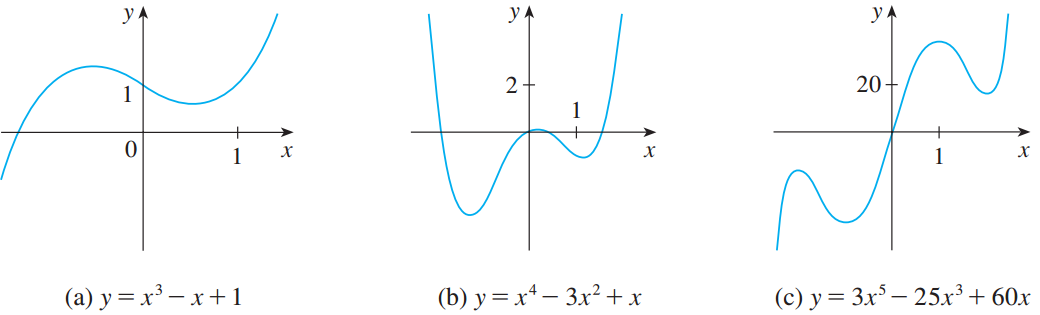
\includegraphics[width=0.7\linewidth]{figures/多项式函数图片}
	\caption{}
	\label{fig:5.1}
\end{figure}
此时我们发现,当多项书次数越高,函数所可以呈现的形状越多。

假设我们现在遇到了一个只知道函数表达式的函数,它的表达复杂诡异,求导的过程十分困难。

而为了实现对此函数的形态研究,我们就需要一个合适的$n$次多项式去拟合这个未知的函数,这就是泰勒出场的背景。

\subsection{从线性拟合到多项式拟合}\label{sec:5.1.2}
从第\ref{ch:3}章知道,对于极其靠近$x_0$的函数,我们用线性函数来近似表达
\begin{equation}
	f(x)\approx f(x_0)+f'(x_0)(x-x_0)\label{eq:5.1}
\end{equation}

那么对于某个区域$I$,需要用多项式去拟合,我们记此多项式为$P_n(x)$,则
\begin{equation}
	P_n(x)=a_0+a_1(x-x_0)+a_x(x-x_0)^2+...+a_n(x-x_0)^n\label{eq:5.2}
\end{equation}

如果实现
\begin{equation*}
	f(x)=P_n(x)+o\qty((x-x_0)^n)
\end{equation*}

即,误差为$(x-x_0)^n$的高阶无穷小,则实现了上述的拟合逼近。

那么如何寻找多项式的系数$a_n$呢\mn{使用牛顿插值法可以推导出泰勒公式的系数,有兴趣的同学自行查阅相关知识点。}?

\section{皮阿诺余项与拉格朗日余项的泰勒展开}

\subsection{带Peano余项的泰勒展开}
\begin{definition}
	\begin{equation}
		f(x)=\sum_{k=0}^n\frac{f^{(k)}(x_0)}{k!}(x-x_0)^k+o\qty((x-x_0)^n)\label{eq:5.3}
	\end{equation}

    像这样的展开称为带Peano余项的泰勒展开。
\end{definition}

此展开可以归结为以下形式:
$$
	f(x)=P_n(x)+R_n(x)
$$

其中,有
$$
P_n(x)=\sum\limits_{k=0}^n\frac{f^{(k)}(x_0)}{k!}(x-x_0)^k,R_n(x)=o((x-x_0)^n)
$$

此处$P_n(x)$称为泰勒多项式,系数称为泰勒系数;$R_n(x)$称为Peano余项,它们合称为带皮阿诺余项的泰勒展开。

\begin{remark}
	对于皮阿诺余项$R_n(x)$,仅能说明这个误差是$(x-x_0)^n)$的高阶无穷大小,不能对于误差大小作具体数值分析。而泰勒定理的另一种表达式,就可以解决这一问题。
\end{remark}

\subsection{带Lagrange余项的泰勒展开}\label{sec:5.2.2}

\begin{definition}
	\begin{equation}
		f(x)=\sum_{k=0}^n\frac{f^{(k)}(x_0)}{k!}(x-x_0)^k+\frac{f^{n+1}(\xi)}{(n+1)!}(x-x_0)^{n+1}\label{eq:5.4}
	\end{equation}

    像这样的展开称为带Lagrange余项的泰勒展开。
\end{definition}

此处$\frac{f^{n+1}(\xi)}{(n+1)!}(x-x_0)^{n+1}$称为拉格朗日余项,也可以写成如下形式:
$$
R_n(x)=\frac{f^{n+1}[x_0+\theta(x-x_0)]}{(n+1)!}(x-x_0)^{n+1},\theta\in(0,1)
$$

使用这一表达,我们就可以通过依据误差精度的需求来确定$n$的大小。

\section{Maclaurin公式}\label{sec:5.3}
学习了泰勒公式的形式之后,其实大家也能看出来,公式形式很复杂而且对于不同的场景有不同的适用情况。为了解决一部分问题,当采取了在0处进行展开的形式后,形成的公式形式方便记忆同时普适性强,我们称之为Maclaurin展开。基本形式如下:

\begin{equation}
    f(x)=f(0)+f'(0)x+\frac{f''(0)}{2!}+\frac{f'''(0)}{3!}+...+\frac{f^{n+1}(\theta x)}{(n+1)!}x^{n+1},~\theta\in(0,1)
    \label{eq:5.5}
\end{equation}

\subsection{需要记忆的常用展开}\label{sec:5.3.1}

\subsubsection{指数函数的展开($x\in(-\infty,+\infty),~\theta\in(0,1)$)}

\begin{equation}
	{\rm e}^x=1+x+\frac{x^2}{2!}+\frac{x^3}{3!}+\frac{x^4}{4!}+\cdots+\frac{x^n}{n!}+\frac{x^{n+1}}{(n+1)!}{\rm e}^{\theta x}\label{eq:5.6}
\end{equation}

\noindent\textbf{记忆技巧:}分子分母数字一致,全是加号。

\subsubsection{正弦函数的展开($x\in(-\infty,+\infty),~\theta\in(0,1)$)}
\begin{equation}
	\sin(x)=x-\frac{x^3}{3!}+\frac{x^5}{5!}-\frac{x^7}{7!}+\cdots+(-1)^{m-1}\frac{x^{2m-1}}{(2m-1))!}+(-1)^m\frac{\cos\theta x}{(2m+1)!}
	\label{eq:5.7}
\end{equation}

\noindent\textbf{记忆技巧:}纯奇数,正负正负交替。

\subsubsection{余弦函数的展开($x\in(-\infty,+\infty),~\theta\in(0,1)$)}
\begin{equation}
	\cos(x)=1-\frac{x^2}{2!}+\frac{x^4}{4!}-\frac{x^6}{6!}+\cdots+(-1)^m\frac{x^{2m}}{(2m)!}+(-1)^{m+1}\frac{\cos\theta x}{(2m+2)!}x^{2m+2}
	\label{eq:5.8}
\end{equation}
\noindent\textbf{记忆技巧:}纯偶数,依然是先正后负,正负正负交替。

\subsubsection{对数函数的展开($x\in(-1,+\infty),~\theta\in(0,1)$)}
\begin{equation}
	\ln(1+x)=x-\frac{x^2}{2}+\frac{x^3}{3}-\frac{x^4}{4}+\cdots+(-1)^{n-1}\frac{x^n}{n}+(-1)^n\frac{x^{n+1}}{(n+1)(1+\theta x)^{n+1}}
	\label{eq:5.9}
\end{equation}
\noindent\textbf{记忆技巧:}正负交替,不用阶乘。

\subsubsection{幂函数的展开($x\in(-1,\infty),\theta\in(0,1)$)}
\begin{equation}
	(1+x)^{\alpha}=1+\alpha x+\frac{\alpha(\alpha-1)}{2!}x^2+\cdots+\frac{\alpha(\alpha-1)\cdots(\alpha-n+1)}{n!}x^{n}+\frac{\alpha(\alpha-1)\cdots(\alpha-n)}{(n+1)!}\frac{x^{n+1}}{(1+\theta x)^{n+1-a}}
\end{equation}

\noindent\textbf{记忆技巧:}对于多项式部分,有$$P_n(x)=\frac{(\alpha)!}{(\alpha-n)!n!}x^n$$


\section{泰勒公式模型、套路、题型}

\subsection{泰勒公式的本质+如何选择Peano/Lagrange余项}
\subsubsection{泰勒公式的本质}
\begin{enumerate}
	\item 用多项式逼近函数。
	\item 用已知点信息表示未知点。
	\item 建立函数与高阶导数的关系。
\end{enumerate}

\subsubsection{如何选择Peano/Lagrange余项}
\begin{enumerate}
	\item 条件不同
	
	Peano:$f(x)$在点$x_0$处有至$n$阶的导数。
	
	Lagrange:$f(x)$在含有$x_0$的开区间$(a,b)$内有$n+1$阶的导数。
	
	\item 余项不同——应用场景不同
	
	Peano:局部的定性分析——求极限,极值
	
	Lagrange:整体的定量分析——求最值,不等式
\end{enumerate}

\subsection{泰勒公式求极限}
\subsubsection{应用泰勒公式统一为多项式}

\begin{problem}
	求$\lim\limits_{x\rightarrow 0}\frac{\cos(x)-{\rm e}^{-\frac{x^2}{2}}}{x^4}$。
	\begin{solution}
		$\cos(x)-{\rm e}^{-\frac{x^2}{2}}$都不好处理\mn{当你遇到极限而不得,如果形式混杂但是函数明晰,欢迎使用泰勒。},用\textbf{泰勒统一为多项式},取皮阿诺展开到与分母同阶或者比分母略高一阶即可。
		
		取Peano展开,$\cos(x)=1-\frac{x^2}{2!}+\frac{x^4}{4!}+o(x^5)$,${\rm e}^{-\frac{x^2}{2}}=1{-\frac{x^2}{2}}+\frac{\qty({-\dfrac{x^2}{2}})^2}{2!}+o_2(x^4)$,代入原式得
		\begin{equation*}
			\lim\limits_{x\rightarrow 0}\frac{1-\dfrac{x^2}{2!}+\dfrac{x^4}{4!}+o(x^5)-\qty[1-\dfrac{x^2}{2}+\dfrac{\qty(-\dfrac{x^2}{2})^2}{2!}+o_2(x^4)]}{x^4}=-\frac{1}{12}+\frac{o(x^4)}{x^4}=-\frac{1}{12}
		\end{equation*}
	\end{solution}
\end{problem}

\subsubsection{通过泰勒公式,从极限中研究函数}
\begin{problem}
	设$f(x)$在$x=0$的某邻域二阶可导,且$\lim\limits_{x\rightarrow 0}\qty(\frac{\sin 3x}{x^3}+\frac{f(x)}{x^2})=0$,则\xparen
	\begin{xchoices}[showanswer=true]
		\item $\lim\limits_{x\rightarrow 0}\qty(\frac{3}{x^2}+\frac{f(x)}{x^2})=0$
		\item $f(0)=3$
		\item $f'(0)=3$
		\item* $f''(0)=9$
	\end{xchoices}
    \vspace{0.5em}
    \begin{solution}
    	这是一个披着极限的外衣,让我们研究函数性态的习题。
    	
    	原式改写为$$\lim\limits_{x\rightarrow 0}\frac{\dfrac{\sin 3x}{x}+f(0)+f'(0)x+\dfrac{f''(0)}{2}x^2+o(x^2)}{x^2}$$
    	
    	注意虽然$\lim\limits_{x\rightarrow 0}\frac{\sin 3x}{x}=3$,但是因为此式下面还有一个$x^2$,所以需要用泰勒改写为$\sin 3x=3x-\frac{(3x)^3}{3!}$,故原式为$$\lim\limits_{x\rightarrow 0}\frac{3-\dfrac{27}{6x^2}+f(0)+f'(0)x+\dfrac{f''(0)}{2}x^2+o(x^2)}{x^2}=0$$
    	
    	则
    	$$\lim\limits_{x\rightarrow 0}\qty[-\frac{9}{2}+\frac{(f(0)+3)+f'(0)x+\dfrac{f''(0)}{2}x^2+o(x^2)}{x^2}]=0$$
    	
    	故\mn{这就是通过极限的必要条件,对于函数性态的研究。}$$f(0)=-3,f'(0)=0,f''(0)=9$$
    \end{solution}
\end{problem}

\begin{problem}
	设$y=f(x)\mbox{在}(-1,1)$内具有二阶连续导数,且$f''(x)\neq 0$,试证:
	\begin{enumerate}[label=(\arabic*)]
		\item 对于$(-1,1)$内的任一$x\neq 0$,存在唯一的$\theta x\in(0,1)$,使$$f(x)=f(0)+xf'\qty(\theta(x)x)$$成立;
		\item  $\lim\limits_{x\rightarrow 0}\theta(x)=\frac{1}{2}$。
	\end{enumerate}
    \begin{proof}
    	\begin{enumerate}[label=(\arabic*)]
    		\item 即证明拉格朗日中值定理在题设条件下的唯一性。
    		
    		由拉格朗日中值定理,得到\mn{这里面的$\theta(x)$表明$\theta$是$x$的函数,没有其他意思}$$f(x)=f(0)+xf\qty(\theta(x)x),~\theta(x)\in(0,1)$$
    		
    		由$f''(x)\neq 0$,得到导函数单调减或者单调增,$\theta$唯一。
    		\item  属于泰勒的变形,十分需要记忆。
    		
    		由二阶可导得$$f(x)=f(0)+f'(0)x+\frac{1}{2}f'(\xi)x^2$$所以$xf\qty(\theta(x)x)=f'(0)+
    		\frac{1}{2}f''(\xi)x^2$,从而$$\lim\limits_{x\rightarrow 0}\theta(x)\frac{f'(\theta(x)x)-f'(0)}{\theta(x)x}=\lim\limits_{x\rightarrow 0}\frac{1}{2}f''(\xi)=\lim\limits_{x\rightarrow 0}\frac{1}{2}f''(0)=\lim\limits_{x\rightarrow 0}\theta(x)f''(0)$$
    		故\mn{见到题设条件又二阶连续导数,某个函数不等于0,要注意应用条件,不要忽略。}$\lim\limits_{x\rightarrow 0}\theta(x)=\frac{1}{2}$
    	\end{enumerate}
    \end{proof}
\end{problem}

\subsection{泰勒公式求解函数性态}
\subsubsection{泰勒公式求解函数最值}
\begin{problem}
	设函数$f(x)$在$[0,1]$上二阶可导,且$f(0)=1,f'(0)=0,f''(1)\leq 1$,试证$f(x)$在$[0,1]$上的最大值不超过$\frac{3}{2}$。
	\begin{solution}
		由于题目中的函数二阶可导,所以泰勒也只能写到二阶\mn{利用泰勒拟合函数,通过已知条件进行放缩。}。
		$$f(x)=1+\frac{f''(\xi)}{2!}x^2\neq 1+\frac{x^2}{2}\leq\frac{3}{2}$$
	\end{solution}
\end{problem}

\subsubsection{泰勒公式求解高阶导数}
\begin{problem}
	求$f(x)=x^2\cdot2^x$在$x=0$处的$n$阶导数$f^n(0)$。
	\begin{solution}
		很显然,如果用泰勒展开成多项式,小于n次方的项求导后消失,大于$n$次方的求导后为0,这也太棒了。
		
		$$f(x)=x^2\cdot2^x=x^2\qty[1+x\ln2+\cdots+\frac{(\ln2)^nx^n}{n!}+o(x^n)]$$
		
		故$x^n$项的系数是$a_n=\frac{(\ln2)^{n-2}}{(n-2)!}$,而$f^n(0)=n!a_n$,故$f^n(0)=n(n-1)(\ln2)^{n-2}$
	\end{solution}
\end{problem}

\subsection{泰勒公式证明不等式}
\begin{problem}
    设$f''(x)>0$,当$x\rightarrow 0$时,$f(x)$和$x$是等价无穷小。证明:当$x\neq 0$时$f(x)>x$。
	\begin{proof}
		由于题目中的函数二阶可导\mn{当出现二阶导数的情况,我们常选用泰勒确定函数性态。},所以泰勒也只能写到二阶。由题意,得到$f(0)=0$,$f'(0)=1$
		$$f(x)=f(0)+f'(0)x+\frac{f''(\xi)}{2!}x^2=x+\frac{f''(\xi)}{2!}x^2>x$$
	\end{proof}
\end{problem}

% \chapter{占位章}
\chapter{函数性态的研究}\label{ch:6}

本节的内容是对前五节内容的综合和提升,在学习过程中,同学们要学以致用,温故知新,具体需要大家:

\begin{enumerate}
	\item \textbf{熟练掌握}函数的极值,单调区间,最值的求法;
	\item \textbf{深刻理解}函数的凹凸性,\textbf{熟练掌握}函数的凹凸区间和拐点的求法;
	\item \textbf{掌握}函数各种渐近线的求法,会大致作出函数的图像。
\end{enumerate}

\section{复习背景}
\subsection{函数的极值}
\begin{definition}
	设有函数$f:I\to\mathbb{R}$,若$\exists\delta>0$,使得$\forall x\in U(x_0,\delta)\subseteq I$,恒有$f(x)\geq f(x_0)(\leq f(x_0))$,则称$f$在$x_0$取得极小(大)值$f(x_0)$。$f$的极小值与极大值统称为$f$的极值,使$f$取得极值点的点$x_0$称为$f$的极值点。
\end{definition}

\begin{remark}
	极值点指的是取得极值时\textbf{自变量的值},并不是极值点的坐标。
\end{remark}

\subsection{Lagrange定理}
\begin{theorem}
	若函数$f:[a,b]\to\mathbb{R}$满足条件:(1)$f$在$[a,b]$连续;\quad(2)$f$在$(a,b)$内可导;则至少存在一点$\xi\in (a,b)$,使
	\begin{equation}
		f(b)-f(a)=f'(\xi)(b-a)\label{eq:6.1}
	\end{equation}
\end{theorem}

\subsection{Taylor定理}
\begin{theorem}
	设函数$f$在区间$I$上$n+1$阶可导,$x_0\in I$,则对任何$x\in I$,在$x$与$x_0$之间至少存在一点$\xi$,使得
	\begin{equation}
		f(x)=\sum^n_{k=0}\frac{f^{(k)}(x_0)}{k!}(x-x_0)^k+\frac{f^{(n+1)}(\xi)}{(n+1)!}(x-x_0)^{n+1}\label{eq:6.2}
	\end{equation}
\end{theorem}
\section{知识点初始——函数的单调性}
设$f:I\to\mathbb{R}$在$I$上连续,在$I$内可导,则以下命题成立:
\begin{enumerate}
	\item $f$在$I$上单调增(减)的充要条件是在$I$内$f'\geq 0$($f'\leq 0$);
	\item 若在$I$内$f'>0$($f'<0$),则$f$在$I$上严格单调增(减)\mn{若$f$在$I$上严格单调增(减),$f'$在$I$内不一定处处为正(负)。}。
\end{enumerate}
\begin{remark}
	为了判定给定函数$f$的单调区间,应当先求出$f'=0$的根以及不可导的点,再分区间讨论函数的单调性。
\end{remark}
\section{知识点初始——函数的极值}
\subsection{函数的驻点}
将使$f'(x)=0$的点称为$f$的驻点,可导函数的极值点必定是驻点。
\subsection{函数极值点的第一条件}
设$f$在$x_0$的某邻域$U(x_0)$内可导,并且$f'(x_0)=0$,
\begin{enumerate}
	\item 若$x<x_0$时$f'(x)\geq 0$,$x>x_0$时$f'(x)\leq 0$,则$f$在$x_0$处取最大值;
	\item 若$x<x_0$时$f'(x)\leq 0$,$x>x_0$时$f'(x)\geq 0$,则$f$在$x_0$处取最小值;
	\item 若$f'(x)$在$x_0$的左右两侧符号不变,则$f$在$x_0$处不取极值。
\end{enumerate}
\begin{remark}
	在讨论极值点时,\textbf{一定不能忽略不可导的点};应当\textbf{利用极值点的定义}来判断不可导的点,这一点在考试中经常作为考点出现。
\end{remark}
\subsection{函数极值点的第二条件}
设$f$在$x_0$处\textbf{二阶可导},并且$f'(x_0)=0,f''(x_0)\neq 0$,则当$f''(x_0)>0(<0)$时,$f$在$x_0$处取极小(大)值。
\subsection{函数极值点的第三条件}
设$f$在$x_0$处\textbf{$n(n\geq 2)$阶可导},并且$f'(x_0)=f''(x_0)=\cdots =f^{(n-1)}(x_0)=0,f^{(n)}(x_0)\neq 0$,
\begin{enumerate}
	\item 当$n$为偶数时,$x_0$必为极值点,若$f^{(n)}(x_0)>0$,则$x_0$为极小值点;若$f^{(n)}(x_0)<0$,则$x_0$为极大值点;
	\item 当$n$为奇数时,$x_0$不是极值点。
\end{enumerate}
\section{知识点初始——函数的最值}
\subsection{函数最值的求法}
若$f\in C[a,b]$,则函数必定在区间上有最值,最值可能出现在:
\begin{enumerate}
	\item 区间内的极值点(可能是驻点或不可导的点);
	\item 区间的端点。
\end{enumerate}

求出极值点,再将其与端点值比较,即可得到最值。
\subsection{函数最值的性质}
区间$I$上的最大值$M$(最小值$m$)有如下性质\mn{该性质也是证明不等式的常用方法之一。}:
\[f(x)\leq M(f(x)\geq m),x\in I\]
\section{知识点初始——函数图像的凹凸性与拐点}
不同教材对凹凸性的定义不同,此处特别说明是从图像的几何特性上定义的。
\subsection{函数图像的凹凸性}
\subsubsection{凹凸性的定义}
\begin{definition}
	设函数$y=f(x)$在区间$I$上连续,若对$I$中任意两点,曲线上对应的弧段始终位于两点连线构成的弦的下(上)方,则称函数$f(x)$在区间$I$中的图像是凹(凸)的。
\end{definition}
\subsubsection{凹凸性的性质}
若$f(x)$在$I$上是凹的,则对$\forall x_1,x_2\in I,\lambda\in (0,1)$,有
\[f(\lambda x_1+(1-\lambda x_2))<\lambda f(x_1)+(1-\lambda)f(x_2)\]

即自变量线性组合的函数值总小于函数的对应线性组合。

\textbf{特别地,当$\lambda =\frac{1}{2}$时},有
\[f(\frac{x_1+x_2}{2})<\frac{f(x_1)+f(x_2)}{2}\]

函数图像为凸的时候有对应性质\mn{函数图像凹凸性的性质在不等式的证明当中经常用到,特别是系数为$\frac{1}{2}$的形式。}。
\subsection{函数的拐点}
\subsubsection{拐点的定义}
\begin{definition}
	连续曲线上凹的图像与凸的图像的转变点称为此曲线的拐点,拐点处二阶导数为0。
\end{definition}
\begin{remark}
	拐点是用\textbf{平面有序数组}表示的,是真正意义上的点,注意与极值点区分。
\end{remark}
\subsubsection{拐点的第一充分条件}
若$f(x)$二阶可导,且$f''(x_0)$为$f''$的变号零点,则$(x_0,f(x_0))$为$f$的拐点。
\subsubsection{拐点的第二充分条件}
若$f(x)$在$x_0$的去心邻域内可导,且$f''$在$x_0$左右变号,则$(x_0,f(x_0))$为$f$的拐点\mn{该条件说明二阶导数不连续的点也有可能是函数的拐点。}。
\subsubsection{拐点的第三充分条件}
若$f(x)$在$U(x_0,\delta)$内三阶可导,且$f''(x_0)=0,f'''(x_0)\neq 0$,则$(x_0,f(x_0))$为$f$的拐点。
\subsubsection{拐点的第四充分条件}
设$f$在$x_0$处\textbf{$n(n\geq 3)$阶可导},并且$f'''(x_0)=f^{(4)}(x_0)=\cdots =f^{(n-1)}(x_0)=0,f^{(n)}(x_0)\neq 0$,
\begin{enumerate}
	\item 当$n$为奇数时,$(x_0,f(x_0))$是拐点;
	\item 当$n$为偶数时,$(x_0,f(x_0))$不是拐点。
\end{enumerate}
\section{函数的渐近线与函数作图}
\subsection{函数的渐近线}
\subsubsection{水平渐近线}
$\lim_{x\to\infty}f(x)=A\xrightarrow{} y=A$为水平渐近线(单侧极限成立即可)。
\subsubsection{铅直渐近线}
$\lim_{x\to a}f(x)=\infty\xrightarrow{}x=a$为铅直渐近线(可以分别求左右极限,一般关注函数的间断点)。
\subsubsection{斜渐近线}
$\lim_{x\to\infty}\frac{f(x)}{x}=k,\quad \lim_{x\to\infty}[f(x)-kx]=b\xrightarrow{}y=kx+b$为斜渐近线(单侧极限成立即可)。
\subsection{函数作图的步骤}
(1)求定义域和间断点;

(2)考察奇偶性,周期性,有界性;

(3)求出一阶导数,二阶导数的零点和不可导的点;

(4)判断单调区间,极值点,凹凸区间,拐点;

(5)求渐近线;

(6)结合特殊位置函数值,描点画图,画出渐近线。
\section{序轴标根法刻画多项式函数的图像}
在遇到高阶多项式以最简因式形式给出时,可以利用该方法大致刻画多项式的形态:

(1)将自变量的系数全部整理为正数;

(2)将函数的零点按数轴位置标在$x$轴上;

(3)若多项式系数为正,自左上方开始由正无穷向下,遇到根的对应因式为奇数次方就穿过,遇到根的对应因式为偶数次方就与它相切,即“奇穿偶切”,经过每一个零点;若多项式系数为负,则图像关于$x$轴对称即可。
\begin{remark}
	(1)读者可以自行探究该方法的原理,在遇到变形时(如加入绝对值)可以灵活应对;
	(2)该方法多用于解决高阶多项式的不等式问题,高阶多项式的极值点,拐点问题。
\end{remark}
\section{证明不等式的常见方法}
(1)利用导数的定义;

(2)利用微分中值定理;

(3)利用函数的单调性;

(4)利用Taylor公式;

(5)利用函数的极值和最值;

(6)利用函数的凹凸性。

\section{习题}
\begin{problem}
	已知$f(x)$在$x=0$某邻域内连续,$\lim_{x\to 0}\frac{f(x)}{1-\cos{x}}=2$,则在$x=0$处$f(x)$\xparen
	\begin{xchoices}[showanswer=true]
		\item 不可导
		\item 可导且$f'(0)\neq 0$
		\item 取得最大值
		\item* 取得最小值
	\end{xchoices}
	\vspace{0.5em}
	\begin{solution}
		由于$\lim_{x\to 0}\frac{f(x)}{1-\cos{x}}=2>0$,由极限的保号性,存在$x=0$的去心邻域,在此去心邻域内$\frac{f(x)}{1-\cos{x}}>0$,又$1-\cos{x}>0$,则在此去心邻域内$f(x)>0$。再由$\lim_{x\to 0}\frac{f(x)}{1-\cos{x}}=2$知,$\lim_{x\to 0}f(x)=0$,又$f(x)$在$x=0$连续,从而$f(0)=0$,则存在$x=0$的邻域,在此邻域内$f(x)\geq f(0)$,则$f(x)$在$x=0$处取极小值,故选(D)
	\end{solution}
\end{problem}
\begin{remark}
	本题\textbf{不能对已知极限用L'Hospital法则},因为原题只假定$f(x)$连续。
\end{remark}

\begin{problem}
	证明:$\tan{x}=1-x$在$(0,1)$内有唯一实根。
	\begin{proof}
		令$f(x)=\tan{x}-1+x$,显然$f(x)$在$[0,1]$上连续,且$f(0)=-1<0,f(1)=\tan{1}>0$,由零点定理知,$f(x)$在$(0,1)$内至少有一个零点,即方程$\tan{x}=1-x$在$(0,1)$内至少有一个实根;又
        \[f'(x)=\sec^2{x}+1>0,\quad x\in [0,1]\]

        则$f(x)$在$(0,1)$上严格单调增,$f(x)$在$(0,1)$内最多一个零点,即方程$\tan{x}=1-x$在$(0,1)$内最多有一个实根;综上方程$\tan{x}=1-x$在$(0,1)$内有且只有一个实根。
	\end{proof}
\end{problem}
\begin{problem}
	设$f''(x)<0,f(0)=0$,证明:对任何$x_1>0,x_2>0$,有$f(x_1+x_2)<f(x_1)+f(x_2)$
	\begin{solution}
		令\[G(x)=f(x_1+x)-f(x)-f(x_1)\]
        \[G'(x)=f'(x_1+x)-f'(x)=f''(\xi)x_1<0\quad(x<\xi <x+x_1)\]

        则$G(x)$单调减,从而有$G(x_2)<G(0)$,即
        \[f(x_1+x_2)-f(x_2)-f(x_1)<f(x_1)-f(0)-f(x_1)=0\]
        \[\Rightarrow f(x_1+x_2)<f(x_1)+f(x_2)\]
	\end{solution}
\end{problem}

\begin{problem}
	设$p,q>0$,且$\frac{1}{p}+\frac{1}{q}=1$,又设$a>0,b>0$,求证:$ab\leq \frac{1}{p}a^p+\frac{1}{q}b^q$。
	\begin{proof}
		对不等式两端同时取对数
        \[\ln{(ab)}\leq \ln{(\frac{1}{p}a^p+\frac{1}{q}b^q)}\]

        令$f(x)=\ln{x},\quad x\in (0,+\infty)$,则$f''(x)=-\frac{1}{x^2},\quad x\in (0,+\infty)$

        $f(x)=\ln{x}$为$(0,+\infty)$上的凹函数,从而有
        \[f\qty(\frac{1}{p}a^p+\frac{1}{q}b^q)\geq \frac{1}{p}f(a^p)+\frac{1}{q}f(b^q)\]
        \[\ln{(\frac{1}{p}a^p+\frac{1}{q}b^q)}\geq \frac{1}{p}a^p+\frac{1}{q}b^q=\ln{a}+\ln{b}=\ln{(ab)}\]
        \[ab\leq \frac{1}{p}a^p+\frac{1}{q}b^q\]
	\end{proof}
\end{problem}

\begin{problem}
	证明不等式
    \[\cos{\sqrt{2}x}<-x^2+\sqrt{1+x^4}\quad x\in (0,\frac{\sqrt{2}}{4}\pi)\]
	\begin{proof}
		令
        \[f(x)=\sqrt{1+x^4}-x^2-\cos{\sqrt{2}x}\]
        \[f'(x)=2x(\frac{x^2}{\sqrt{1+x^4}}-1)+\sqrt{2}\sin{\sqrt{2}x}\]

        由Taylor展开式,易得
        \[\sin{x}>x-\frac{1}{3!}x^3(x>0)\]

        所以
        \[f'(x)>2x(\frac{x^2}{\sqrt{1+x^4}}-1)+2x-\frac{2x^3}{3}=\frac{2x^3}{\sqrt{1+x^4}}-\frac{2x^3}{3}>0\]

        因此,当$x\in (0,\frac{\sqrt{2}}{4}\pi)$时,$f(x)$单调增加,又$f(0)=0$,所以$f(x)>0$。
	\end{proof}
\end{problem}
\newpage
\begin{problem}[思考题]
	证明\textbf{赫尔德不等式}:设实数$\alpha,\beta$满足$\frac{1}{\alpha}+\frac{1}{\beta}=1$,且$a_i,b_i(i=1,\cdots,n)$为非负实数,则当$\alpha>1$时
    \[\sum^n_{i=1}a_i b_i\leq (\sum^n_{i=1}a^\alpha_i)^{\frac{1}{\alpha}}(\sum^n_{i=1}b^\beta_i)^{\frac{1}{\beta}}\]

    当$\alpha<1$时
    \[\sum^n_{i=1}a_i b_i\geq (\sum^n_{i=1}a^\alpha_i)^{\frac{1}{\alpha}}(\sum^n_{i=1}b^\beta_i)^{\frac{1}{\beta}}\]
\end{problem}

\begin{proof}
	记$p_i=b_i^\beta$,由$\frac{1}{\alpha}+\frac{1}{\beta}=1$易得,当$\alpha<1$时,原不等式等价于
	\[\sum^n_{i=1}a_i p_i^{1-\frac{1}{\alpha}}\leq (\sum^n_{i=1}a^\alpha_i)^{\frac{1}{\alpha}}(\sum^n_{i=1}p_i)^{1-\frac{1}{\alpha}}\]

	等价于
	\[\sum^n_{i=1}(\frac{p_i}{\sum^n_{i=1}p_i})\alpha_i p_i^{-\frac{1}{\alpha}}\leq (\sum^n_{i=1}(\frac{a_i^\alpha}{\sum^n_{i=1}p_i}))^{\frac{1}{\alpha}}\]

	记$x_i=a_i p_i^{-\frac{1}{\alpha}},\lambda_i=\frac{p_i}{\sum^n_{i=1}p_i}$,则上面不等式化为
	\[(\sum^n_{i=1}\lambda_i x_i)^\alpha\leq \sum^n_{i=1}\lambda_i x_i^\alpha\]

	且$\sum^n_{i=1}\lambda_i=1$,故只需讨论函数$f(x)=x^\alpha(\alpha>1)$的凸性。

	令$f(x)=x^\alpha,\quad x\geq 0$,则$f''(x)=\alpha(\alpha-1)x^\alpha$,当$\alpha>1$时,$f''(x)>0$,$f(x)$是下凸函数。

	对任意一组非负实数$p_i(i=1,\cdots,n)$,记$\lambda_i=\frac{p_i}{\sum^n_{i=1}p_i}$,则$\sum^n_{i=1}\lambda_i=1$,对任意$x_i\geq 0$,利用凸函数的Jensen不等式,得
	\[(\sum^n_{i=1}\lambda_i x_i)^\alpha\leq \sum^n_{i=1}\lambda_i x_i^\alpha\]
	
	即
	\[\qty(\sum^n_{i=1}\frac{p_i x_i}{\sum^n_{i=1}p_i})^\alpha\leq \sum^n_{i=1}\frac{p_i x_i}{\sum^n_{i=1}p_i}\]
	
	即
	\[\sum^n_{i=1}p_i x_i\leq \qty(\sum^n_{i=1}a^\alpha_i)^{\frac{1}{\alpha}}\qty(\sum^n_{i=1}p_i)^{1-\frac{1}{\alpha}}\]

	取$a_i=p_i^{\frac{1}{\alpha}},b_i=p_i^{\frac{1}{\beta}}$,则有
	\[\sum^n_{i=1}a_i b_i\leq \qty(\sum^n_{i=1}a^\alpha_i)^{\frac{1}{\alpha}}\qty(\sum^n_{i=1}b^\beta_i)^{\frac{1}{\beta}}\]
	
	同理可证$\alpha<1$的情况。
\end{proof}

\begin{remark}
	(1)当$\alpha=\beta=2$时,赫尔德不等式即为常见的\textbf{柯西不等式};

	(2)凸函数的\textbf{Jensen不等式}:

	设$f(x)\in C(I)$,则$f(x)$是$I$上下凸函数的充要条件为:$\forall x_i\in I,\forall \lambda\in(0,1)(i=1,\cdots,n)$,且$\sum^n_{i=1}\lambda_i=1$,恒有
	\[f\qty(\sum^n_{i=1}\lambda_i x_i)\leq \sum^n_{i=1}\lambda_i f(x_i)\]
\end{remark}

\backmatter
\pagestyle{back}
% %---------------------------------------------------------------------------
% % 附录
% %---------------------------------------------------------------------------

\appendix
\phantomsection
% 修改附录部分的章节样式
\makeatletter
\let\oldmakeschapterhead\@makeschapterhead
\renewcommand{\@makeschapterhead}[1]{
	\addtocontents{toc}{\protect\hypertarget{app:\theappendix}{}}%  跳转回目录
	\checkoddpage
	\@ifoddpage{ % 奇数页
		\begin{tikzpicture}[remember picture,overlay]
			\node at (current page.north west)
			{
				\begin{tikzpicture}[remember picture,overlay]
					\draw[fill=lbdeepblue,draw opacity=0]
					++(0,-2cm) rectangle ++(\paperwidth,-4pt);
					\node[color=lbdeepgreen,inner sep=12pt,below left] (chapter)
					at  +(\paperwidth-1.2cm,-2cm) {\Huge\titlefont\fontspec{Palatino-Roman}
							\protect\hyperlink{app:\theappendix}{\theappendix}};
					\draw[line width=2pt,color=lbgreen]
					++(\paperwidth-1.2cm,0) |- ($(chapter.south west)+(0,4pt)$);
					\node[color=lbdeepblue,left=7pt,anchor=north east] at (chapter.south east)
					{
						\parbox[c][][c]{18cm}
						{\flushright\Huge\bfseries\titlefont\fontspec{Palatino-Roman}
							\texorpdfstring{\protect\hyperlink{app:\theappendix}{#1}}{#1}}
					};
				\end{tikzpicture}
			};
		\end{tikzpicture}
		\vspace{7cm}
		% \renewcommand{\chaptermark}[1]{\markboth{\normalfont\kaiti \theappendix\; #1}{}}%
		% \renewcommand{\sectionmark}[1]{\markright{{\pplj\thesection}\quad #1}}%
    \renewcommand{\chaptermark}[1]{\markboth{\normalfont\kaiti%
    \protect\hyperlink{app:\theappendix}{\theappendix\; #1}%
    }%
    {}%
    }%
		\chaptermark{#1}%
	}{ % 偶数页
		\begin{tikzpicture}[remember picture,overlay]
			\node at (current page.north west)
			{
				\begin{tikzpicture}[remember picture,overlay]
					\draw[fill=lbdeepblue,draw opacity=0]
					++(0,-2cm) rectangle ++(\paperwidth,-4pt);
					\node[color=lbdeepgreen,inner sep=12pt,below right] (chapter)
					at  +(1.2cm,-2cm) {\Huge\titlefont\fontspec{Palatino-Roman}
							\protect\hyperlink{app:\theappendix}{\theappendix}};
					\draw[line width=2pt,color=lbgreen]
					++(1.2cm,0) |- ($(chapter.south east)+(0,4pt)$);
					\node[color=lbdeepblue,right=7pt,anchor=north west] at (chapter.south west)
					{
						\parbox[c][][c]{18cm}
						{\flushleft\Huge\bfseries\titlefont\fontspec{Palatino-Roman}
							\texorpdfstring{\protect\hyperlink{app:\theappendix}{#1}}{#1}}
					};
				\end{tikzpicture}
			};
		\end{tikzpicture}
		\vspace{7cm}
		% \renewcommand{\chaptermark}[1]{\markboth{\normalfont\kaiti \theappendix\; #1}{}}%
		% \renewcommand{\sectionmark}[1]{\markright{{\pplj\thesection}\quad #1}}%
    \renewcommand{\chaptermark}[1]{\markboth{\normalfont\kaiti%
    \protect\hyperlink{app:\theappendix}{\theappendix\; #1}%
    }%
    {}%
    }%
		\chaptermark{#1}%
	}
}
\let\newmakeschapterhead\@makeschapterhead
\makeatother

\renewcommand{\thechapter}{\Alph{appendix}}   % 修改chapter的样式
\numberwithin{equation}{chapter}               % 让公式编号跟随chapter编号

\appendixchapter{基本初等函数的导数公式表}\label{app:1}

{\small
\noindent\begin{tblr}{X[c]X[c]}
    \toprule[lbdeepgreen]
	{\color{lbdeepgreen}$f(x)$} & {\color{lbdeepgreen}$f'(x)$} \\  \midrule[lbgreen]
	$C$ & 0 \\
	\hline[dashed,lbgreen]
	$x^{\mu}$ & $\mu x^{\mu -1}$ \\
	\hline[dashed,lbgreen]
	$a^x$ & $a^x\ln{a}$ \\
	${\rm e}^x$ & ${\rm e}^x$ \\
	\hline[dashed,lbgreen]
	$\log_a{x}$ & $\frac{1}{x\ln{a}}$ \\
	$\ln{x}$ & $\frac{1}{x}$ \\
	\hline[dashed,lbgreen]
	$\sin{x}$ & $\cos{x}$ \\
	$\cos{x}$ & $-\sin{x}$ \\
	$\tan{x}$ & $\sec^2{x}$ \\
	$\cot{x}$ & $-\csc^2{x}$ \\
	$\sec{x}$ & $\sec{x}\tan{x}$ \\
	$\csc{x}$ & $-\csc{x}\cot{x}$ \\
	\hline[dashed,lbgreen]
	$\arcsin{x}$ & $\frac{1}{\sqrt{1-x^2}}$ \\
	$\arccos{x}$ & $-\frac{1}{\sqrt{1-x^2}}$ \\
	$\arctan{x}$ & $\frac{1}{1+x^2}$ \\
	$\arccot{x}$ & $-\frac{1}{1+x^2}$ \\
	\bottomrule[lbdeepgreen]
\end{tblr}}

\newpage
%\input{content/app2.tex}
%\input{content/app3.tex}
%\input{content/app4.tex}
%\input{content/app5.tex}
% 附录文件的最后都要加上\newpage,否则目录页码会出错

% %---------------------------------------------------------------------------
% % Index
% %---------------------------------------------------------------------------

% \printindex

% 封底
%--------------------------------------------------------------------------
\setcounter{tp}{\value{TotPages}+2}
\bookmark[page=\value{tp}, level=-1]{封底}
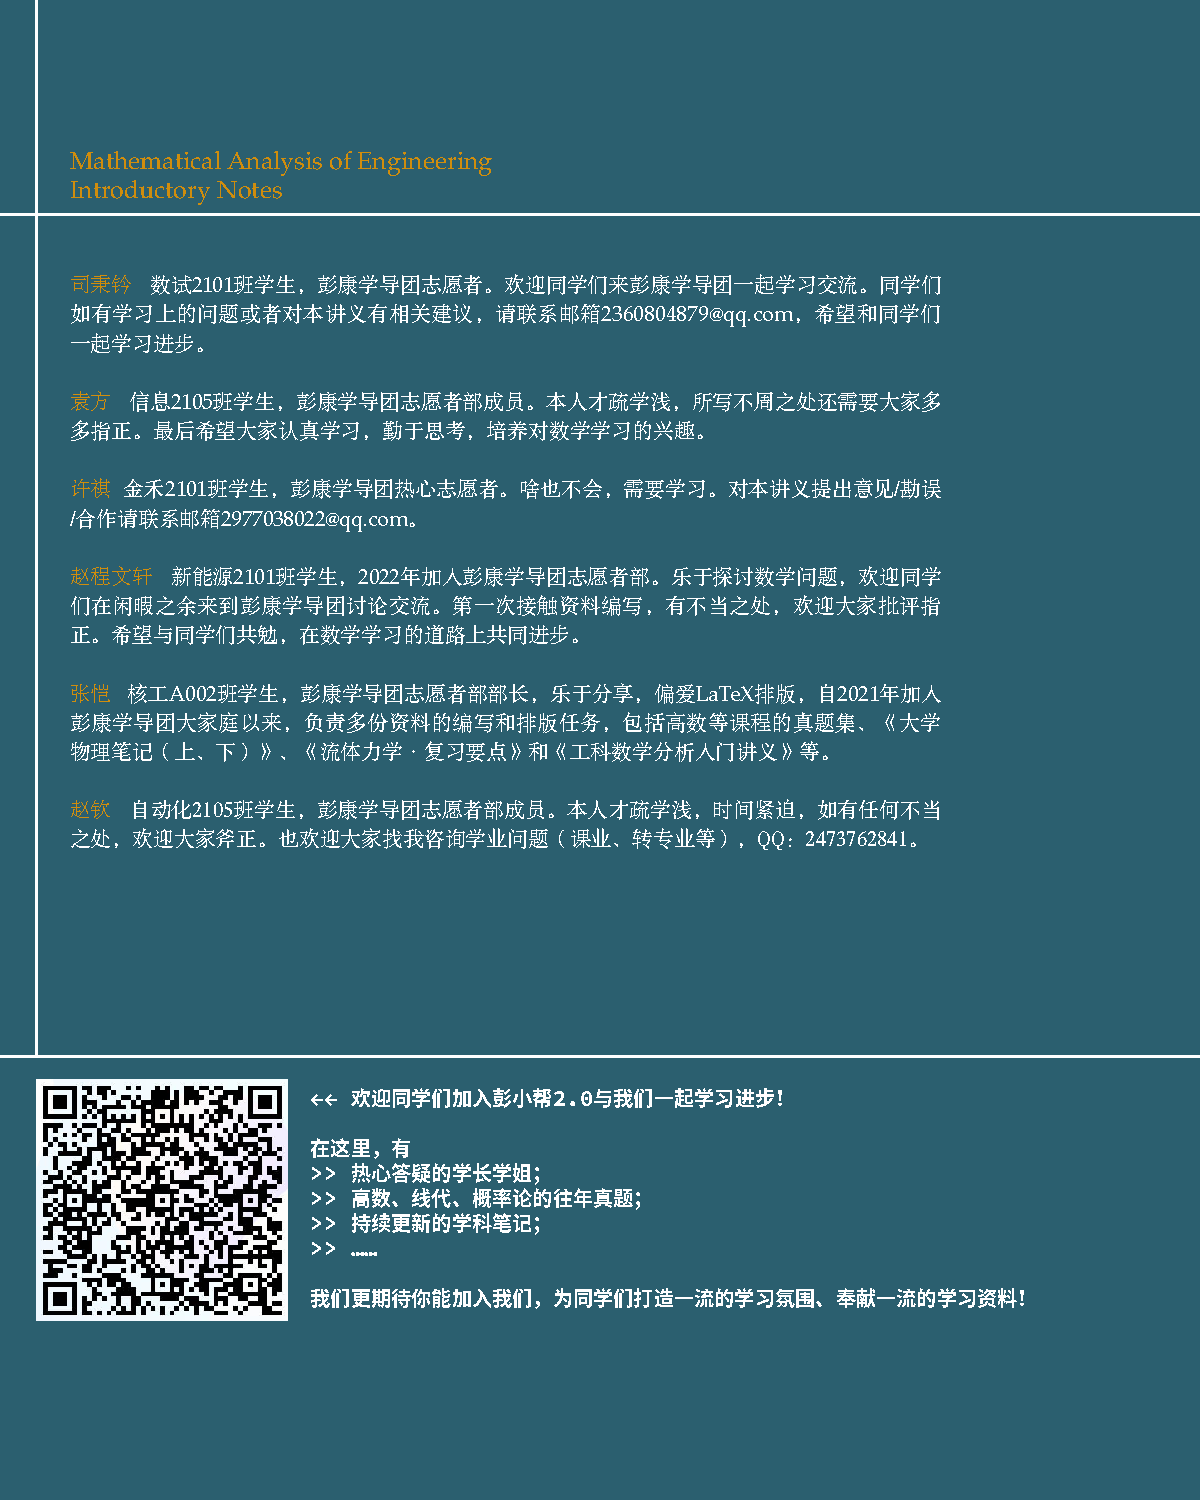
\includepdf[noautoscale=true, width=\paperwidth]{backcover.pdf}
\end{document}
